\documentclass{scrartcl}

\usepackage{todonotes}
\usepackage{graphicx}
\usepackage{hyperref}
\usepackage{float}
\usepackage{siunitx}

\usepackage{booktabs}
\usepackage{threeparttable}
\usepackage{xspace}
\usepackage{multirow}
\usepackage{makecell}
\usepackage{tabularx}

\usepackage{tablefootnote}

\usepackage{geometry}
\geometry{top=2cm, bottom=2cm, left=2.5cm, right=2.5cm}

\usepackage{listings}
\lstset{
  basicstyle=\ttfamily\footnotesize,
  mathescape
}

%\usepackage[left=3cm, right=3cm, bottom=3cm, top=3cm]{geometry}

\usepackage{dirtree}
\usepackage{tikz}
\usepackage{figures/tikz-timing}
\usepackage{circuitikz}
\usepackage{xcolor}
\usetikzlibrary{shapes.symbols}

\newcommand{\core}{\texttt{smaesh\_hpc}}
\newcommand{\clk}{\ensuremath{\texttt{clk}}}
\newcommand{\rst}{\ensuremath{\texttt{syn\_rst}}}
\newcommand{\svrsInValid}{\ensuremath{\texttt{in\_valid}}} % remove
\newcommand{\svrsInDataValid}{\ensuremath{\texttt{in\_data\_valid}}}
\newcommand{\svrsInReady}{\ensuremath{\texttt{in\_ready}}} %Rremove 
\newcommand{\svrsInDataReady}{\ensuremath{\texttt{in\_data\_ready}}}
\newcommand{\svrsPlaintext}{\ensuremath{\texttt{in\_shares\_plaintext}}} % remove
\newcommand{\svrsInData}{\ensuremath{\texttt{in\_shares\_data}}}
\newcommand{\svrsKey}{\ensuremath{\texttt{in\_key\_data}}}
\newcommand{\svrsKeyValid}{\ensuremath{\texttt{in\_key\_valid}}}
\newcommand{\svrsKeyReady}{\ensuremath{\texttt{in\_key\_ready}}}
\newcommand{\svrsKeySizeCfg}{\ensuremath{\texttt{in\_key\_size\_cfg}}}
\newcommand{\svrsKeyModeInverse}{\ensuremath{\texttt{in\_key\_mode\_inverse}}}
\newcommand{\svrsCiphertext}{\ensuremath{\texttt{out\_shares\_ciphertext}}} % remove
\newcommand{\svrsOutData}{\ensuremath{\texttt{out\_shares\_data}}}
\newcommand{\svrsOutValid}{\ensuremath{\texttt{out\_valid}}}
\newcommand{\svrsOutReady}{\ensuremath{\texttt{out\_ready}}}
\newcommand{\svrsSeed}{\ensuremath{\texttt{in\_seed}}}
\newcommand{\svrsSeedValid}{\ensuremath{\texttt{in\_seed\_valid}}}
\newcommand{\svrsSeedReady}{\ensuremath{\texttt{in\_seed\_ready}}}

\newcommand{\topName}{\ensuremath{\texttt{smaesh\_hpc}}}
\newcommand{\topModAES}{\ensuremath{\texttt{MSKaes\_32bits\_core}}}
\newcommand{\topModPRNG}{\ensuremath{\texttt{prng\_top}}}
\newcommand{\topModKHOLD}{\ensuremath{\texttt{MSKkey\_holder}}}
\newcommand{\topModReseedCtrl}{\ensuremath{\texttt{reseed\_controller}}}
\newcommand{\topModsvrsCtrl}{\ensuremath{\texttt{reseed\_controller}}}
\newcommand{\SB}{\ensuremath{\texttt{SubBytes}}}
\newcommand{\SR}{\ensuremath{\texttt{ShiftRows}}}
\newcommand{\MC}{\ensuremath{\texttt{MixColumns}}}
\newcommand{\AK}{\ensuremath{\texttt{AddRoundKey}}}

\newcommand{\KEYSIZE}{\ensuremath{\texttt{KEYSIZE}}}

% Ports of AES core
\newcommand{\portAESInValid}{\ensuremath{\texttt{valid\_in}}}
\newcommand{\portAESInReady}{\ensuremath{\texttt{in\_ready}}}
\newcommand{\portAESInPlaintext}{\ensuremath{\texttt{sh\_plaintext}}} % remove
\newcommand{\portAESInData}{\ensuremath{\texttt{sh\_in\_data}}}
\newcommand{\portAESInKey}{\ensuremath{\texttt{sh\_key}}}
\newcommand{\portAESbusy}{\ensuremath{\texttt{busy}}}
\newcommand{\portAESOutValid}{\ensuremath{\texttt{out\_valid}}}
\newcommand{\portAESOutReady}{\ensuremath{\texttt{out\_ready}}}
\newcommand{\portAESOutData}{\ensuremath{\texttt{sh\_out\_data}}} 
\newcommand{\portAESOutCipher}{\ensuremath{\texttt{sh\_ciphertext}}} % remove
\newcommand{\portAESRnd}{\ensuremath{\texttt{rnd}}}
\newcommand{\portAESRndReady}{\ensuremath{\texttt{in\_rnd\_ready}}}

\newcommand{\portAESKeySize}{\ensuremath{\texttt{in\_key\_size\_cfg}}}

\newcommand{\portAESLastKeyCol}{\ensuremath{\texttt{sh\_last\_key\_col}}}
\newcommand{\portAESLastKeyColPreValid}{\ensuremath{\texttt{last\_key\_pre\_valid}}}
\newcommand{\portAESRndRfValid}{\ensuremath{\texttt{rnd\_bus0\_valid\_for\_rfrsh}}}
\newcommand{\portAESModeI}{\ensuremath{\texttt{mode\_192}}}
\newcommand{\portAESModeII}{\ensuremath{\texttt{mode\_256}}}
\newcommand{\portAESInverse}{\ensuremath{\texttt{inverse}}}
\newcommand{\portAESKSchedOnly}{\ensuremath{\texttt{key\_schedule\_only}}}


% Ports of PRNG 
\newcommand{\portPrngSeed}{\ensuremath{\texttt{in\_seed}}}
\newcommand{\portPrngStartReseed}{\ensuremath{\texttt{start\_reseed}}}
\newcommand{\portPrngOutReady}{\ensuremath{\texttt{out\_ready}}}
\newcommand{\portPrngOutValid}{\ensuremath{\texttt{out\_valid}}}
\newcommand{\portPrngOutRnd}{\ensuremath{\texttt{out\_rnd}}}
\newcommand{\portPrngBusy}{\ensuremath{\texttt{busy}}}

\newcommand{\triviumKey}{\ensuremath{\texttt{key}[79:0]}}
\newcommand{\triviumIV}{\ensuremath{\texttt{IV}[79:0]}}
\newcommand{\triviumInState}{\ensuremath{1 | 1 | 1 | 0^{112} | \triviumIV | 0^{13} | \triviumKey}}
\newcommand{\triviumOut}{\ensuremath{\texttt{stream}}}

% Ports of KHolder
\newcommand{\portKHDataIn}{\ensuremath{\texttt{data\_in}}}
\newcommand{\portKHDataInValid}{\ensuremath{\texttt{data\_in\_valid}}}
\newcommand{\portKHDataInReady}{\ensuremath{\texttt{data\_in\_ready}}}
\newcommand{\portKHLastKeyCol}{\ensuremath{\texttt{sh\_last\_key\_col}}}
\newcommand{\portKHLastKeyColPreValid}{\ensuremath{\texttt{sh\_last\_key\_col\_pre\_valid}}}
\newcommand{\portKHDataOut}{\ensuremath{\texttt{sh\_data\_out}}}
\newcommand{\portKHRndIn}{\ensuremath{\texttt{rnd\_rfrsh\_in}}}
\newcommand{\portKHRndInValid}{\ensuremath{\texttt{rnd\_rfrsh\_in\_valid}}}
\newcommand{\portKHStartFetch}{\ensuremath{\texttt{start\_fetch\_procedure}}}
\newcommand{\portKHSizeCfg}{\ensuremath{\texttt{key\_size\_cfg}}}
\newcommand{\portKHModeInverse}{\ensuremath{\texttt{mode\_inverse}}}
\newcommand{\portKHBusy}{\ensuremath{\texttt{busy}}}
\newcommand{\portKHAESbusy}{\ensuremath{\texttt{aes\_busy}}}
\newcommand{\portKHLastKeyReq}{\ensuremath{\texttt{last\_key\_computation\_required}}}
\newcommand{\portKHModeII}{\ensuremath{\texttt{aes\_mode\_256}}}
\newcommand{\portKHModeI}{\ensuremath{\texttt{aes\_mode\_192}}}
\newcommand{\portKHInInverse}{\ensuremath{\texttt{mode\_inverse}}}
\newcommand{\portKHInverse}{\ensuremath{\texttt{aes\_mode\_inverse}}}



% AES submodule
\newcommand{\modAESdpState}{\ensuremath{\texttt{MSKaes\_32bits\_state\_datapath}}}
\newcommand{\modAESdpKey}{\ensuremath{\texttt{MSKaes\_32bits\_key\_datapath}}}
\newcommand{\modAESsbox}{\ensuremath{\texttt{MSKSbox}}}

\newcommand{\AESsboxIn}{\ensuremath{\texttt{bytes\_to\_SB}}}
\newcommand{\AESsboxOut}{\ensuremath{\texttt{bytes\_from\_SB}}}
\newcommand{\AESsboxRnd}{\ensuremath{\texttt{rnd}}}
\newcommand{\AESsboxValidIn}{\ensuremath{\texttt{sbox\_valid\_in}}}
\newcommand{\AESsboxValidOut}{\ensuremath{\texttt{sbox\_valid\_out}}}
\newcommand{\AESsboxFeedKey}{\ensuremath{\texttt{feed\_sb\_key}}}
\newcommand{\AESFetchIn}{\ensuremath{\texttt{tap\_top\_input}}}

\newcommand{\AESdpStatePlaintext}{\ensuremath{\texttt{sh\_plaintext}}}
\newcommand{\AESdpStateFromSB}{\ensuremath{\texttt{sh\_4bytes\_from\_SB}}}
\newcommand{\AESdpStateFromKey}{\ensuremath{\texttt{sh\_4bytes\_from\_key}}}
\newcommand{\AESdpStateToSB}{\ensuremath{\texttt{sh\_4bytes\_to\_SB}}}
\newcommand{\AESdpStateCiphertext}{\ensuremath{\texttt{sh\_ciphertext}}}

\newcommand{\AESdpKeyKey}{\ensuremath{\texttt{sh\_key}}}
\newcommand{\AESdpKeyToSB}{\ensuremath{\texttt{sh\_4bytes\_rot\_to\_SB}}}
\newcommand{\AESdpKeyFromSB}{\ensuremath{\texttt{sh\_4bytes\_rot\_from\_SB}}}
\newcommand{\AESdpKeyToAK}{\ensuremath{\texttt{sh\_4bytes\_to\_AK}}}
\newcommand{\AESdpKeyToAKInverse}{\ensuremath{\texttt{sh\_3bytes\_to\_AK\_inverse}}}

\newcommand{\AESdpStateFromKeyInverse}{\ensuremath{\texttt{sh\_3bytes\_from\_key}}}


% dpState internal
\newcommand{\dpStateModMC}{\ensuremath{\texttt{MC\_unit}}}
\newcommand{\dpStateModMCInv}{\ensuremath{\texttt{MC\_unit}^{-1}}}
\newcommand{\dpStateByteToMC}{\ensuremath{\texttt{a}}}
\newcommand{\dpStateByteFromMC}{\ensuremath{\texttt{b}}}
\newcommand{\dpStateCtrlRouteMC}{\ensuremath{\texttt{route\_MC}}}
\newcommand{\dpStateCtrlRouteLoop}{\ensuremath{\texttt{loop}}}
\newcommand{\dpStateCtrlRouteIn}{\ensuremath{\texttt{init}}}
\newcommand{\dpStateCtrlEnable}{\ensuremath{\texttt{state\_enable}}}

\newcommand{\dpStateToSBForward}{\ensuremath{\texttt{sh\_4bytes\_toSB\_forward}}}
\newcommand{\dpStateToMCInverse}{\ensuremath{\texttt{sh\_4bytes\_toMC\_inverse}}}
\newcommand{\dpStateCtrlEnableKAdd}{\ensuremath{\texttt{enable\_key\_add}}}
\newcommand{\dpStateCtrlEnableKAddInverse}{\ensuremath{\texttt{enable\_key\_add\_inverse}}}
\newcommand{\dpStateCtrlEnableKAddDual}{\ensuremath{\texttt{enable\_key\_add\_dual}}}
\newcommand{\dpStateToSBReverse}{\ensuremath{\texttt{sh\_4bytes\_toSB\_inverse}}}

\newcommand{\dpStateCtrlBypassMCInverse}{\ensuremath{\texttt{bypass\_MC\_inverse}}}
\newcommand{\dpStateCtrlEnableToSBInverse}{\ensuremath{\texttt{en\_toSB\_inverse}}}


% dpKey internal
\newcommand{\dpKeyCtrlInit}{\ensuremath{\texttt{init}}}
\newcommand{\dpKeyCtrlLoop}{\ensuremath{\texttt{loop}}}
\newcommand{\dpKeyCtrlRouteScan}{\ensuremath{\texttt{\dpKeyCtrlInit||\dpKeyCtrlLoop}}}
\newcommand{\dpKeyCtrlRouteInit}{\dpKeyCtrlInit}
\newcommand{\dpKeyCtrlRouteLoop}{\dpKeyCtrlLoop}
\newcommand{\dpKeyCtrlRouteFromSB}{\ensuremath{\texttt{from\_SB}}}
\newcommand{\dpKeyCtrlEnable}{\ensuremath{\texttt{KH\_enable}}}

\newcommand{\dpKeyCtrlRstBuffer}{\ensuremath{\texttt{rst\_buffer}}}
\newcommand{\dpKeyCtrlFBFromHigh}{\ensuremath{\texttt{FB\_from\_high}}}
\newcommand{\dpKeyCtrlReverseDefaut}{\ensuremath{\texttt{dec128}}}
\newcommand{\dpKeyCtrlColSevenToSB}{\ensuremath{\texttt{col7\_to\_SB}}}
\newcommand{\dpKeyCtrlDisableRot}{\ensuremath{\texttt{disable\_rot\_rcon}}}

%% Time only
\newcommand{\timeCnrRound}{\ensuremath{\texttt{cnt\_round}}}
\newcommand{\timeCnrCycle}{\ensuremath{\texttt{cnt\_fsm}}}
\newcommand{\timeCnrExecCycles}{\ensuremath{\texttt{cnt\_cycles}}}

%%% Pseudo code 
\newcommand{\pP}[1]{\ensuremath{\texttt{P}_{#1}}}
\newcommand{\pK}[1]{\ensuremath{\texttt{K}_{#1}}}
\newcommand{\pCt}[1]{\ensuremath{\texttt{C}_{#1}}}
\newcommand{\pS}[2]{\ensuremath{\texttt{S}_{#1}^{#2}}}
\newcommand{\pRK}[2]{\ensuremath{\texttt{RK}_{#1}^{#2}}}

\newcommand{\pSB}[2]{\ensuremath{\texttt{SB}_{#1}^{#2}}}
\newcommand{\pSR}[2]{\ensuremath{\texttt{SR}_{#1}^{#2}}}
\newcommand{\pMC}[2]{\ensuremath{\texttt{MC}_{#1}^{#2}}}
\newcommand{\pAK}[2]{\ensuremath{\texttt{AK}_{#1}^{#2}}}

\newcommand{\pR}[2]{\ensuremath{\texttt{R}_{#1}^{#2}}}
\newcommand{\pRSB}[2]{\ensuremath{\texttt{RSB}_{#1}^{#2}}}
\newcommand{\SW}[1]{\ensuremath{\texttt{SubWord}(#1)}}

\newcommand{\RCON}[1]{\ensuremath{\texttt{RCON}^{#1}}}

\newcommand{\Nr}{\ensuremath{\mathsf{Nr}}}

%% if for debug puprose
\newif\ifemptytime
\emptytimetrue
\emptytimefalse

% Parametric generation of signals
\def\cHalfPeriod{1} 
\pgfmathsetmacro{\cPeriod}{\cHalfPeriod * 2}
\def\scaleFontTime{1.0}

%% Pipe data routing font Size
\newcommand{\pipeFS}{\scriptsize}
\newcommand{\cDP}[1]{\cPeriod D{\ifemptytime  \else \pipeFS \scalebox{\scaleFontTime}{ #1 } \fi}}
\newcommand{\NcDP}[2]{#2{\cPeriod D}{\ifemptytime  \else \pipeFS \scalebox{\scaleFontTime} { #1 } \fi}}

%% Pipeline dp Key
\newcommand{\dpKeyDFF}[1]{\ensuremath{\texttt{sh\_m\_key[#1]}}}

\newcommand{\timeStartdpKey}[1]{D{}\cDP{\pRK{#1}{i-1}}}
\newcommand{\timeFivedpKey}[4]{\NcDP{\pRK{#1}{i-1}}{1}\cDP{\pRK{#2}{i-1}}\cDP{\pRK{#3}{i-1}}\cDP{\pRK{#4}{i-1}}}
\newcommand{\timePartdpKey}[4]{\cDP{\pRK{#2}{i-1}}\cDP{\pRK{#3}{i-1}}\cDP{\pRK{#4}{i-1}}}
\newcommand{\timeStopdpKey}[2]{\NcDP{\pRK{#1}{i}}{1}\cDP{\pRK{#2}{i}}}

\newcommand{\timeMidIdpKey}[4]{\NcDP{\pRK{#1}{i}}{1}\cDP{\pRK{#2}{i}}\cDP{\pRK{#3}{i}}\cDP{\pRK{#4}{i}}}
\newcommand{\timeMidIIdpKey}[4]{\NcDP{\pRK{#1}{i-1}}{1}\cDP{\pRK{#2}{i-1}}\cDP{\pRK{#3}{i-1}}\cDP{\pRK{#4}{i}}}
\newcommand{\timeMidIIIdpKey}[4]{\NcDP{\pRK{#1}{i-1}}{1}\cDP{\pRK{#2}{i-1}}\cDP{\pRK{#3}{i}}\cDP{\pRK{#4}{i}}}
\newcommand{\timeMidIIIIdpKey}[4]{\NcDP{\pRK{#1}{i-1}}{1}\cDP{\pRK{#2}{i}}\cDP{\pRK{#3}{i}}\cDP{\pRK{#4}{i}}}

\newcommand{\timeLinedpKeyI}[4]{\timeStartdpKey{#4}\timeFivedpKey{#1}{#2}{#3}{#4}\timeMidIdpKey{#1}{#2}{#3}{#4}\timeStopdpKey{#1}{#2}}
\newcommand{\timeLinedpKeyII}[4]{\timeStartdpKey{#4}\timeFivedpKey{#1}{#2}{#3}{#4}\timeMidIIdpKey{#1}{#2}{#3}{#4}\timeStopdpKey{#1}{#2}}
\newcommand{\timeLinedpKeyIII}[4]{\timeStartdpKey{#4}\timeFivedpKey{#1}{#2}{#3}{#4}\timeMidIIIdpKey{#1}{#2}{#3}{#4}\timeStopdpKey{#1}{#2}}
\newcommand{\timeLinedpKeyIIII}[4]{\timeStartdpKey{#4}\timeFivedpKey{#1}{#2}{#3}{#4}\timeMidIIIIdpKey{#1}{#2}{#3}{#4}\timeStopdpKey{#1}{#2}}

%% Pipeline dp State
\newcommand{\dpStateDFF}[1]{\ensuremath{\texttt{sh\_reg\_out[#1]}}}

% Start
\newcommand{\timeStInterndpStateXII}[4]{D{}\cDP{\pMC{#3}{i-1}}\cDP{\pMC{#4}{i-1}}\cDP{\pMC{#1}{i-1}}\cDP{\pS{#2}{i}}\cDP{\pS{#3}{i}}\NcDP{\pS{#4}{i}}{2}}
\newcommand{\timeStInterndpStateXIII}[4]{D{}\cDP{\pMC{#3}{i-1}}\cDP{\pMC{#4}{i-1}}\cDP{\pMC{#1}{i-1}}\cDP{\pMC{#2}{i-1}}\cDP{\pS{#3}{i}}\NcDP{\pS{#4}{i}}{2}}
\newcommand{\timeStInterndpStateXIV}[4]{D{}\cDP{\pMC{#3}{i-1}}\cDP{\pMC{#4}{i-1}}\cDP{\pMC{#1}{i-1}}\cDP{\pMC{#2}{i-1}}\cDP{\pMC{#3}{i-1}}\NcDP{\pS{#4}{i}}{2}}
\newcommand{\timeStInterndpStateXV}[4]{D{}\cDP{\pMC{#3}{i-1}}\cDP{\pMC{#4}{i-1}}\cDP{\pMC{#1}{i-1}}\cDP{\pMC{#2}{i-1}}\cDP{\pMC{#3}{i-1}}\NcDP{\pMC{#4}{i-1}}{2}}

\newcommand{\timeStInterndpStateVIII}[4]{D{}\cDP{\pMC{#3}{i-1}}\cDP{\pMC{#4}{i-1}}\cDP{\pMC{#1}{i-1}}\cDP{\pMC{#2}{i-1}}\cDP{\pS{#3}{i}}\NcDP{\pS{#4}{i}}{2}}
\newcommand{\timeStInterndpStateIX}[4]{D{}\cDP{\pMC{#3}{i-1}}\cDP{\pMC{#4}{i-1}}\cDP{\pMC{#1}{i-1}}\cDP{\pMC{#2}{i-1}}\cDP{\pMC{#3}{i-1}}\NcDP{\pS{#4}{i}}{2}}
\newcommand{\timeStInterndpStateX}[4]{D{}\cDP{\pMC{#3}{i-1}}\cDP{\pMC{#4}{i-1}}\cDP{\pMC{#1}{i-1}}\cDP{\pMC{#2}{i-1}}\cDP{\pMC{#3}{i-1}}\NcDP{\pMC{#4}{i-1}}{2}}
\newcommand{\timeStInterndpStateXI}[4]{D{}\cDP{\pMC{3}{i-1}}\cDP{\pMC{7}{i-1}}\cDP{\pMC{#1}{i-1}}\cDP{\pS{#2}{i}}\cDP{\pS{#3}{i}}\NcDP{\pS{#4}{i}}{2}}

\newcommand{\timeStInterndpStateIV}[4]{D{}\cDP{\pS{#3}{i-1}}\cDP{\pMC{#4}{i-1}}\cDP{\pMC{#1}{i-1}}\cDP{\pMC{#2}{i-1}}\cDP{\pMC{#3}{i-1}}\NcDP{\pS{#4}{i}}{2}}
\newcommand{\timeStInterndpStateV}[4]{D{}\cDP{\pS{#3}{i-1}}\cDP{\pMC{#4}{i-1}}\cDP{\pMC{#1}{i-1}}\cDP{\pMC{#2}{i-1}}\cDP{\pMC{#3}{i-1}}\NcDP{\pMC{#4}{i-1}}{2}}
\newcommand{\timeStInterndpStateVI}[4]{D{}\cDP{\pS{#3}{i-1}}\cDP{\pMC{#4}{i-1}}\cDP{\pMC{#1}{i-1}}\cDP{\pS{#2}{i}}\cDP{\pS{#3}{i}}\NcDP{\pS{#4}{i}}{2}}
\newcommand{\timeStInterndpStateVII}[4]{D{}\cDP{\pS{#3}{i-1}}\cDP{\pMC{#4}{i-1}}\cDP{\pMC{#1}{i-1}}\cDP{\pMC{#2}{i-1}}\cDP{\pS{#3}{i}}\NcDP{\pS{#4}{i}}{2}}

\newcommand{\timeStInterndpStateIII}[4]{D{}\cDP{\pS{#3}{i-1}}\cDP{\pS{#4}{i-1}}\cDP{\pMC{#1}{i-1}}\cDP{\pMC{#2}{i-1}}\cDP{\pMC{#3}{i-1}}\NcDP{\pS{#4}{i}}{2}}
\newcommand{\timeStInterndpStateII}[4]{D{}\cDP{\pS{#3}{i-1}}\cDP{\pS{#4}{i-1}}\cDP{\pMC{#1}{i-1}}\cDP{\pMC{#2}{i-1}}\cDP{\pS{#3}{i}}\NcDP{\pS{#4}{i}}{2}}
\newcommand{\timeStInterndpStateI}[4]{D{}\cDP{\pS{#3}{i-1}}\cDP{\pS{#4}{i-1}}\cDP{\pMC{#1}{i-1}}\cDP{\pS{#2}{i}}\cDP{\pS{#3}{i}}\NcDP{\pS{#4}{i}}{2}}
\newcommand{\timeStInterndpStateZ}[4]{D{}\cDP{\pS{#3}{i-1}}\cDP{\pS{#4}{i-1}}\cDP{\pMC{#1}{i-1}}\cDP{\pMC{#2}{i-1}}\cDP{\pMC{#3}{i-1}}\NcDP{\pMC{#4}{i-1}}{2}}

% End 
\newcommand{\timeEndInterndpStateXII}[4]{\cDP{\pMC{#2}{i}}\cDP{\pMC{#3}{i}}\cDP{\pMC{#4}{i}}\cDP{\pMC{#1}{i}}\cDP{\pS{#2}{i+1}}}
\newcommand{\timeEndInterndpStateXIII}[4]{\cDP{\pMC{#2}{i}}\cDP{\pMC{#3}{i}}\cDP{\pMC{#4}{i}}\cDP{\pMC{#1}{i}}\cDP{\pMC{#2}{i}}}

\newcommand{\timeEndInterndpStateXI}[4]{\NcDP{\pMC{#1}{i-1}}{1}\cDP{\pMC{#3}{i}}\cDP{\pMC{#4}{i}}\cDP{\pMC{#1}{i}}\cDP{\pS{#2}{i+1}}}
\newcommand{\timeEndInterndpStateX}[4]{\NcDP{\pS{#1}{i}}{1}\cDP{\pMC{#3}{i}}\cDP{\pMC{#4}{i}}\cDP{\pMC{#1}{i}}\cDP{\pMC{#2}{i}}}

\newcommand{\timeEndInterndpStateIV}[4]{\NcDP{\pS{#1}{i}}{1}\cDP{\pS{#2}{i}}\cDP{\pMC{#4}{i}}\cDP{\pMC{#1}{i}}\cDP{\pMC{#2}{i}}}
\newcommand{\timeEndInterndpStateV}[4]{\NcDP{\pS{#1}{i}}{1}\cDP{\pS{#2}{i}}\cDP{\pMC{#4}{i}}\cDP{\pMC{#1}{i}}\cDP{\pMC{#2}{i}}}
\newcommand{\timeEndInterndpStateVI}[4]{\NcDP{\pMC{#1}{i-1}}{1}\cDP{\pS{#2}{i}}\cDP{\pMC{#4}{i}}\cDP{\pMC{#1}{i}}\cDP{\pS{#2}{i+1}}}
\newcommand{\timeEndInterndpStateVII}[4]{\NcDP{\pS{#1}{i}}{1}\cDP{\pMC{#2}{i-1}}\cDP{\pMC{#4}{i}}\cDP{\pMC{#1}{i}}\cDP{\pMC{#2}{i}}}

\newcommand{\timeEndInterndpStateZ}[4]{\NcDP{\pS{#1}{i}}{1}\cDP{\pS{#2}{i}}\cDP{\pS{#3}{i}}\cDP{\pMC{#1}{i}}\cDP{\pS{#2}{i+1}}}
\newcommand{\timeEndInterndpStateI}[4]{\NcDP{\pMC{#1}{i-1}}{1}\cDP{\pS{#2}{i}}\cDP{\pS{#3}{i}}\cDP{\pMC{#1}{i}}\cDP{\pS{#2}{i+1}}}
\newcommand{\timeEndInterndpStateII}[4]{\NcDP{\pS{#1}{i}}{1}\cDP{\pMC{#2}{i-1}}\cDP{\pS{#3}{i}}\cDP{\pMC{#1}{i}}\cDP{\pS{#2}{i+1}}}
\newcommand{\timeEndInterndpStateIII}[4]{\NcDP{\pS{#1}{i}}{1}\cDP{\pS{#2}{i}}\cDP{\pMC{#3}{i-1}}\cDP{\pMC{#1}{i}}\cDP{\pMC{#2}{i}}}

% Full line
\newcommand{\timeLinedpStateXII}[4]{\timeStInterndpStateXII{#1}{#2}{#3}{#4}\timeEndInterndpStateXII{#1}{#2}{#3}{#4}}
\newcommand{\timeLinedpStateXIII}[4]{\timeStInterndpStateXIII{#1}{#2}{#3}{#4}\timeEndInterndpStateXIII{#1}{#2}{#3}{#4}}
\newcommand{\timeLinedpStateXIV}[4]{\timeStInterndpStateXIV{#1}{#2}{#3}{#4}\timeEndInterndpStateXIII{#1}{#2}{#3}{#4}}
\newcommand{\timeLinedpStateXV}[4]{\timeStInterndpStateXV{#1}{#2}{#3}{#4}\timeEndInterndpStateXIII{#1}{#2}{#3}{#4}}

\newcommand{\timeLinedpStateVIII}[4]{\timeStInterndpStateVIII{#1}{#2}{#3}{#4}\timeEndInterndpStateX{#1}{#2}{#3}{#4}}
\newcommand{\timeLinedpStateIX}[4]{\timeStInterndpStateIX{#1}{#2}{#3}{#4}\timeEndInterndpStateX{#1}{#2}{#3}{#4}}
\newcommand{\timeLinedpStateX}[4]{\timeStInterndpStateX{#1}{#2}{#3}{#4}\timeEndInterndpStateX{#1}{#2}{#3}{#4}}
\newcommand{\timeLinedpStateXI}[4]{\timeStInterndpStateXI{#1}{#2}{#3}{#4}\timeEndInterndpStateXI{#1}{#2}{#3}{#4}}

\newcommand{\timeLinedpStateIV}[4]{\timeStInterndpStateIV{#1}{#2}{#3}{#4}\timeEndInterndpStateIV{#1}{#2}{#3}{#4}}
\newcommand{\timeLinedpStateV}[4]{\timeStInterndpStateV{#1}{#2}{#3}{#4}\timeEndInterndpStateV{#1}{#2}{#3}{#4}}
\newcommand{\timeLinedpStateVI}[4]{\timeStInterndpStateVI{#1}{#2}{#3}{#4}\timeEndInterndpStateVI{#1}{#2}{#3}{#4}}
\newcommand{\timeLinedpStateVII}[4]{\timeStInterndpStateVII{#1}{#2}{#3}{#4}\timeEndInterndpStateVII{#1}{#2}{#3}{#4}}

\newcommand{\timeLinedpStateZ}[4]{\timeStInterndpStateZ{#1}{#2}{#3}{#4}\timeEndInterndpStateZ{#1}{#2}{#3}{#4}}
\newcommand{\timeLinedpStateI}[4]{\timeStInterndpStateI{#1}{#2}{#3}{#4}\timeEndInterndpStateI{#1}{#2}{#3}{#4}}
\newcommand{\timeLinedpStateII}[4]{\timeStInterndpStateII{#1}{#2}{#3}{#4}\timeEndInterndpStateII{#1}{#2}{#3}{#4}}
\newcommand{\timeLinedpStateIII}[4]{\timeStInterndpStateIII{#1}{#2}{#3}{#4}\timeEndInterndpStateIII{#1}{#2}{#3}{#4}}

%% PRNG section
\newcommand{\NRNDBITS}{\ensuremath{\texttt{NRNDBITS}}}
\newcommand{\MULHPCRND}{\ensuremath{\texttt{MUL\_HPC2\_RND}}}
\newcommand{\NTRIVIUMS}{\ensuremath{\texttt{NTRIVIUMS}}}
\newcommand{\UNROLL}{\ensuremath{\texttt{UNROLL}}}
\newcommand{\MAXUNROLL}{\ensuremath{\texttt{PRNG\_MAX\_UNROLL}}}


\usepackage{pgf}

% Debug to print label to nodes
\newif\ifdebug
\debugtrue
\debugfalse

%%%% CONFIG
\def\debugFontSize{\tiny}
%%%%


%% Debug node
% #1: test
% #2: position
\newcommand{\debugN}[2][]{
    \node at #2 {\ifdebug o \else \fi};
    \node [above] at #2 {\debugFontSize \ifdebug #1 \else \fi};
}

% Basic rectangle:
% #1: draw param
% #2: uid
% #3: center
% #4: width 
% #5: height
% #6: amount of nodes on W side
% #7: amount of nodes on E side
% #8: amount of nodes on N side
% #9: amount of nodes on S side
\newcommand{\rectangle}[9][]{
    \coordinate (#2/TL) at ($#3 + (-#4/2,#5/2)$);
    \coordinate (#2/TR) at ($#3 + (#4/2,#5/2)$);
    \coordinate (#2/BL) at ($#3 + (-#4/2,-#5/2)$);
    \coordinate (#2/BR) at ($#3 + (#4/2,-#5/2)$);
    \draw [#1] (#2/TL) -- (#2/TR)%
    -- (#2/BR) -- (#2/BL) -- (#2/TL); 
    % Draw the nodes on side W
    \foreach \xi in {1,...,#6}{
        \pgfmathsetmacro\offy{(#5)/(#6+1)}
        \pgfmathsetmacro\yval{\xi*\offy}
        \coordinate (#2/W\xi) at ($(#2/TL) - (0,\yval)$);
        \debugN[W\xi]{(#2/W\xi)}
    }
    % Draw the nodes on side E
    \foreach \xi in {1,...,#7}{
        \pgfmathsetmacro\offy{(#5)/(#7+1)}
        \pgfmathsetmacro\yval{\xi*\offy}
        \coordinate (#2/E\xi) at ($(#2/TR) - (0,\yval)$);
        \debugN[E\xi]{(#2/E\xi)}
    }
    % Draw the nodes on side N
    \foreach \xi in {1,...,#8}{
        \pgfmathsetmacro\offx{(#4)/(#8+1)}
        \pgfmathsetmacro\xval{\xi*\offx}
        \coordinate (#2/N\xi) at ($(#2/TL) + (\xval,0)$);
        \debugN[N\xi]{(#2/N\xi)}
    }
    % Draw the nodes on side S
    \foreach \xi in {1,...,#9}{
        \pgfmathsetmacro\offx{(#4)/(#9+1)}
        \pgfmathsetmacro\xval{\xi*\offx}
        \coordinate (#2/S\xi) at ($(#2/BL) + (\xval,0)$);
        \debugN[S\xi]{(#2/S\xi)}
    }
    %%%
    \coordinate (#2/center) at #3;
    \coordinate (#2/south) at ($#3 - (0,#5/2)$);
    \coordinate (#2/north) at ($#3 + (0,#5/2)$);
}

%% Rectangle from corner locations
% #1: draw param
% #2: uid
% #3: TR pos
% #4: BL pos
% #5: amount of nodes on W side
% #6: amount of nodes on E side
% #7: amount of nodes on N side
% #8: amount of nodes on S side
\newcommand{\rectangleC}[8][]{
    % Extract width/height from the corners
    \coordinate (sizerC) at ($#3-#4$); 
    % Define coordinate for remaining cornes
    \path let \p1=(sizerC) in coordinate (TL) at ($#4+(0,\y1)$);
    \path let \p1=(sizerC) in coordinate (BR) at ($#4+(\x1,0)$);
    % Draw the rectange
    \draw [#1] #3 |- #4 #3 -| #4;
    % Draw the node on side W
    \foreach \xi in {1,...,#5}{
        \pgfmathsetmacro\propL{\xi/(#5+1)}
        \coordinate (#2/W\xi) at ($(TL)!\propL!#4$);
        \debugN[W\xi]{(#2/W\xi)}
    }
    % Draw the node on side E
    \foreach \xi in {1,...,#6}{
        \pgfmathsetmacro\propL{\xi/(#6+1)}
        \coordinate (#2/E\xi) at ($#3!\propL!(BR)$);
        \debugN[E\xi]{(#2/E\xi)}
    }
    % Draw the node on side N
    \foreach \xi in {1,...,#7}{
        \pgfmathsetmacro\propL{\xi/(#7+1)}
        \coordinate (#2/N\xi) at ($(TL)!\propL!#3$);
        \debugN[N\xi]{(#2/N\xi)}
    }
    % Draw the node on side S
    \foreach \xi in {1,...,#8}{
        \pgfmathsetmacro\propL{\xi/(#8+1)}
        \coordinate (#2/S\xi) at ($#4!\propL!(BR)$);
        \debugN[S\xi]{(#2/S\xi)}
    }
    % Generate general coordinate
    \coordinate (#2/TL) at (TL);
    \coordinate (#2/TR) at #3;
    \coordinate (#2/BL) at #4;
    \coordinate (#2/BR) at (BR);
    \coordinate (#2/center) at ($#3!0.5!#4$);
    \coordinate (#2/south) at ($(#2/BL)!0.5!(#2/BR)$);
}

% Flip-Flop
% 1: draw style
% 2: id 
% 3: loc
% 4: width
% 5: height
\newcommand{\DFF}[5][]{
    % Draw a rectangle
    \rectangle[#1]{rect}{#3}{#4}{#5}{1}{1}{1}{1}
    % Draw the triangle
    \pgfmathsetmacro\baseT{(#4)/3}
    \pgfmathsetmacro\baseTd{\baseT/2}
    \pgfmathsetmacro\heightT{(#5)/7}
    \coordinate (TC0) at ($(rect/south) - (\baseTd,0)$);
    \coordinate (TC1) at ($(rect/south) + (\baseTd,0)$);
    \coordinate (TC2) at ($(rect/south) + (0,\heightT)$);
    \draw [#1] (TC0) -- (TC2) -- (TC1);
    \coordinate (#2/D) at (rect/W1);
    \coordinate (#2/Q) at (rect/E1);
    \coordinate (#2/center) at #3;
    \coordinate (#2/north) at (rect/N1);
}

% XOR
% 1: draw style
% 2: id
% 3: loc
% 4: radius
\newcommand{\XOR}[4][]{
    % Draw a circle    
    \draw [#1] #3 circle (#4);
    % Generate coordinate for th xor
    \coordinate (#2/north) at ($#3 + (0,#4)$);
    \coordinate (#2/south) at ($#3 + (0,-#4)$);
    \coordinate (#2/east) at ($#3 + (#4,0)$);
    \coordinate (#2/west) at ($#3 + (-#4,0)$);
    \coordinate (#2/center) at ($#3$);
    \draw [#1] (#2/north) -- (#2/south);
    \draw [#1] (#2/west) -- (#2/east);
}


%


\title{SMAesH: technical documentation}
\subtitle{Masked Hardware AES with HPC}
\author{SIMPLE-Crypto}
\date{}

\begin{document}
\definecolor{colorIN}{RGB}{255,0,0}
\definecolor{colorOUT}{RGB}{0,0,255}
\definecolor{colorSEED}{RGB}{0,100,32}




\maketitle

\tableofcontents

\section{Overview}
\label{section:overview}
This document describes SIMPLE-Crypto's Masked AES in Hardware (SMAesH),
implemented in the $\topName$ hardware IP. 

\section{History}
\begin{description}
    \item[2.0.0 (2024-10-08)] Major (breaking API) update: add AES-192, AES-256 and decryption .
    \item[1.1.0 (2024-09-02)] 4 cycles Canright S-box (new optimized architecture).
    \item[1.0.1 (2023-06-15)] Fix latency in Section 5.4 (documentation change only).
    \item[1.0.0 (2023-05-01)] Initial release.
\end{description}

\section{Features}
The \core{} module is a masked hardware implementation of the three variants of
the AES algorithm as specified in \cite{nist197}. In particular, the core
implements the encryption as well as the decryption for the variants using
128-bit, 192-bit and 256-bit keys.  

\begin{itemize}
\item{The core implements the AES-128, AES-192, AES-256 encryption and decryption function, chosen dynamically at run-time.}
\item{The implementation is protected against side-channel attacks using a combination of HPC1~\cite{DBLP:journals/tc/CassiersGLS21} and HPC3~\cite{DBLP:conf/ccs/Knichel022} masking scheme.}
\item{The core relies on an internal long-term key, configured at run-time. The key configuration also defines the execution performed by the core (e.g., encryption vs decryption or algorithm version used).}
\item{The amount of shares $d\ge 2$ can be chosen at synthesis time.\footnote{While feasible, the architecture of the S-box is optimized and automatically generated for a given amount of shares. Therefore, changing the amount of share without re-generating the S-box may lead to suboptimal results. See~\ref{section:masked_aes_core_arhcitecture} for more details.}}
\item{The randomness required for the masking scheme is internally generated using an embedded PRNG.}
\item{The core is controlled through four simple valid-ready stream interfaces (input key, input data, output data and PRNG seed.}
\item{The core has an encryption latency of 86, 201 and 118 cycles for respectively AES-128, AES-192 and AES-256. The corresponding throughput is one 128-bit block of data per 86, 201 and 118 cycles.}
\item{The core has a decryption latency of 86, 121 and 118 cycles for respectively AES-128, AES-192 and AES-256. The corresponding throughput is one 128-bit block of data per 86, 121 and 118 cycles.}
\item{A key change comes with a latency penalty of $16d$ cycles. For decryption only, an additional penalty of $16$ cycles plus the latency of an encryption is paid.}
\item{The state of the core is automatically cleared when encryption finishes.}
\item{The key is automatically refreshed after each usage without latency penalty.}
\item{The AES-192 version comes together with the AES-256 version without paying additional logic other than control.}
\item{The AES-192 and AES-256 version can be disabled at synthesis time. }
\end{itemize}

\section{Core User Guide} 
\label{section:svrs_usage}

A top-level view of the core is shown in Figure~\ref{fig:top_module_view_ports}
and a detailed list of the ports is given in Table~\ref{table:ports}.  The
interface is composed of four independent interfaces: the key configuration
input (in violet), the input plaintext/ciphertext (in red), the
ciphertext/plaintext output (in blue) and the PRNG seed (in green).
The key (\svrsKey) is a 32-bit bus while the input (\svrsInData) and the output (\svrsOutData)
are 128-bit masked values.
The internal PRNG seed (\svrsSeed) is 80-bit wide.

\begin{figure}
    \centering
    \resizebox{\textwidth}{!}{
        \small
        \begin{tikzpicture}
            % width of Ports IOs
\def\arrowIOWidth{0.5mm}
\def\xshIO{1.0cm}

% Ports for basic IO port
\newcommand{\portW}[4][]{
    \node[xshift=-\xshIO,anchor=east,text=#4] (port) at (#2) {#3};
    \draw [#1,line width=\arrowIOWidth] (port.east) -- (#2);
}
\newcommand{\portE}[4][]{
    \node[xshift=\xshIO,anchor=west,text=#4] (port) at (#2) {#3};
    \draw [#1,line width=\arrowIOWidth] (#2) -- (port);
}
\newcommand{\portN}[4][]{
    \node[yshift=\xshIO,anchor=south,text=#4] (port) at (#2) {#3};
    \draw [#1,line width=\arrowIOWidth] (port) -- (#2);
}

% Draw rectangle
\rectangle[line width=0.5mm]{main}{(0,0)}{4}{6}{8}{8}{2}{0};
% Add module name
\draw (main/center) node {\topName};
% Add ports inputs
\portW[->]{main/W1}{\svrsInValid}{colorIN}
\portW[<-]{main/W2}{\svrsInReady}{colorIN}
\portW[->]{main/W3}{\svrsPlaintext[128d-1:0]}{colorIN}
\portW[->]{main/W4}{\svrsKey[128d-1:0]}{colorIN}

\portW[->]{main/W6}{\svrsSeedValid}{colorSEED}
\portW[<-]{main/W7}{\svrsSeedReady}{colorSEED}
\portW[->]{main/W8}{\svrsSeed[79:0]}{colorSEED}
% Add ports outputs 
\portE[->]{main/E1}{\svrsOutValid}{colorOUT}
\portE[<-]{main/E2}{\svrsOutReady}{colorOUT}
\portE[->]{main/E3}{\svrsCiphertext[128d-1:0]}{colorOUT}
% Add port control
\portN[->]{main/N1}{\clk}{black}
\portN[->]{main/N2}{\rst}{black}


        \end{tikzpicture}
    }
    \caption{Top level view of module $\topName$.}
    \label{fig:top_module_view_ports}
\end{figure}

\begin{table}
    \centering
    \begin{threeparttable}
        \footnotesize
        \setlength{\tabcolsep}{1ex}
        \begin{tabularx}{\textwidth}{@{}ccccX@{}}
            \toprule
            \multicolumn{5}{c}{\textbf{Module Generics}} \\
            \thead{Parameter} & & \thead{Value Type} & & \thead{Description} \\
            \midrule
            $d$ & & integer & & Amount of shares \\
            $\MAXUNROLL$ & & integer & & Maximum unrolling for the embedded PRNG. \\
            \midrule
            \multicolumn{5}{c}{\textbf{Module Ports}} \\
            \thead{Ports Name} & \thead{Type} & \thead{Direction} & \thead{Width [bits]} & \thead{Description} \\
            \midrule
             %&  &  &  &  \\
             \texttt{clk} & clock & input & $1$ & Clock (all the logic is synchronized on the positive edge). \\
             \texttt{syn\_rst} & control & input & $1$ & Active high synchronous reset. Keep asserted for at least one cycle. \\
             \addlinespace[2ex]
             \multicolumn{5}{c}{\color{colorKEY} SVRS Key interface} \\
             \svrsKey & data & input & 32 & Key share material (SVRS \texttt{data} signal). \\
             \svrsKeySizeCfg & control & input & 2 & Key size configuration. \\ 
                            &   & & & - 2'b0: 128-bit \\
                            &   & & & - 2'b1: 192-bit \\
                            &   & & & - 2'b2: 256-bit \\
             \svrsKeyModeInverse & control & input & 1 & Active high inverse mode configuration. \\
             \svrsKeyValid & control & input & 1 & SVRS \texttt{valid} signal. \\
             \svrsKeyReady & control & output & 1 & SVRS \texttt{ready} signal. \\
             \addlinespace[2ex]
             \multicolumn{5}{c}{\color{colorIN} SVRS Input interface} \\
             \svrsInData & data & input & $128d$ & Shared plaintext/ciphertext (SVRS \texttt{data} signal). \\
             \svrsInDataValid & control & input & $1$ & SVRS \texttt{valid} signal. \\
             \svrsInDataReady & control & output & $1$ & SVRS \texttt{ready} signal. \\
             \addlinespace[2ex]
             \multicolumn{5}{c}{\color{colorSEED} SVRS Seed interface} \\
             \svrsSeed & data & input & $80$ & Fresh randomness used as a seed by the embedded PRNG (SVRS \texttt{data} signal). \\
             \svrsSeedValid & control & input & $1$ & SVRS \texttt{valid} signal. \\
             \svrsSeedReady & control & output & $1$ & SVRS \texttt{ready} signal. \\
             \addlinespace[2ex]
             \multicolumn{5}{c}{\color{colorOUT} SVRS Output interface} \\
             \svrsCiphertext & data & output & $128d$ & Shared ciphertext (SVRS \texttt{data} signal). \\
             \svrsOutValid & control & output & $1$ & SVRS \texttt{valid} signal. \\
             \svrsOutReady & control & input & $1$ & SVRS \texttt{valid} signal. \\
            \bottomrule
        \end{tabularx}
        \caption{$\topName$ port description.}%
        \label{table:ports} 
    \end{threeparttable}
\end{table}

% & & & &  \\


In this section we next detail the operation of the Synchronous Valid-Ready
Stream (SVRS) protocol for the data interfaces, the operation of the $\topName$
core, and the masked data encoding.

\subsection{SVRS protocol}

\begin{figure}
    \centering
    \begin{tikztimingtable}
        \texttt{clock} & L 6{HL} \\
        \texttt{data} & X XX{} 3{DD}{}XXXX \\
        \texttt{valid} & L LL 3{HH} LLLL \\
        \texttt{ready} & L 3{LL} HH LLLL \\
        \extracode
        \makeatletter
        \begin{pgfonlayer}{background}
            \begin{scope}[gray,semitransparent,semithick]
                \foreach \x in {1,3,...,11}
                \draw (\x,1.5) -- (\x,-6.5);
            \end{scope}
        \end{pgfonlayer}
    \end{tikztimingtable}
    \caption{SVRS transaction (don't care (X) signals are represented with a flat red solid line).}
    \label{fig:basic_svrs}
\end{figure}


\begin{figure}
    \centering
    \begin{tikztimingtable}
        \texttt{clock} & L 13{HL} \\
        \texttt{data} & X 1{XX}{} 2{DD}{} 1{DD}{} 1{XX} {} 3{DD}{} 3{XX} DD XX \\ 
        \texttt{valid} & L 1{LL} 3{HH} 1{LL} 3{HH} 1{LL} 2{LL} 1{HH} LL\\
        \texttt{ready} & L 2{LL} 3{HH} 2{LL} 1{HH} 1{LL} 3{HH} 1{LL}\\
        \extracode
        \makeatletter
        \begin{pgfonlayer}{background}
            \begin{scope}[gray,semitransparent,semithick]
                \foreach \x in {1,3,...,25}
                \draw (\x,1.5) -- (\x,-6.5);
            \end{scope}
        \end{pgfonlayer}
    \end{tikztimingtable}
    \caption{Multiple SVRS transactions.}
    \label{fig:seq_svrs}
\end{figure}

The Synchronous Valid-Ready Stream (SVRS) protocol operates between a sender and a receiver.
The bus is composed of the two control signals \texttt{valid} and \texttt{ready}, as well as any number of \texttt{data} wires.
The \texttt{valid} and \texttt{data} signals are outputs (resp. inputs) of the
sender (resp. receiver), while the \texttt{ready} signal is an input (resp.
output) of the sender (resp. receiver).

The bus operates synchronously with an event source shared by the sender and
the receiver (here, the positive edges of the clock).
At each event, a transaction occurs if both \texttt{valid} and \texttt{ready}
are asserted (i.e. set to logical~1). The transmitted data of the transaction is
the value of the \texttt{data} signals at the event.

Once \texttt{valid} is asserted, it cannot be de-asserted (i.e., sticky signal), nor can the value of
\texttt{data} be changed until a transaction occurs.
To prevent deadlocks, a sender must not wait until the assertion of
\texttt{ready} before asserting \texttt{valid}.
To prevent combinational logic loops, the \texttt{valid} signal may not
combinationally depend on the \texttt{ready} signal.

Examples of protocol use are given in Figures~\ref{fig:basic_svrs} and~\ref{fig:seq_svrs}.


\subsection{Core Usage}
\label{section:core_usage}

\paragraph{Key configuration}
An new key is configured in the core by executing several transactions on the
key interfaces.  The configuration of a key of $\KEYSIZE$ bits (128, 192 or
256) is done by performing $d\cdot\KEYSIZE / 32$ transactions.  Each
transaction allows transferring 32 bits of key share. The transactions must be
performed such that the key shares are transferred sequentially, 32-bit word per
32-bit word, from the least significant word to the most significant one. The
key size and the inverse configuration are specified during the first
transaction. These configurations will then be hold internally to the core in
order to configure all the executions following the key configuration. In order
to configure the core in decryption mode, the signal $\svrsKeyModeInverse$
signal must be asserted during the first transaction. in such case, the core
internally computes the key of the last round after having fetched the key
value and stores it as the long term key.  
The Figure~\ref{fig:srvs_key_cfgd2} depicts an example of key configuration for the 128-bit key
$\texttt{umsk\_key}$, encoded in the 2-shares sharings $\texttt{share0\_key}$ and
$\texttt{share1\_key}$.   

\begin{figure}
    \centering
    \def\scaleFont{0.5}
    \begin{tikztimingtable}
        \texttt{\texttt{umsk\_key}} & 17{DD}{0x0f0e0d0c\_0b0a0908\_07060504\_03020100} \\
        \texttt{\texttt{share0\_key}} & 17{DD}{0x2a082ca6\_58197c74\_6395f678\_7f02d885} \\
        \texttt{\texttt{share1\_key}} & 17{DD}{0x250621aa\_5313757c\_6493f37c\_7c00d985} \\
        \\
        \texttt{clock} & L 17{HL} \\
        \svrsKey & X  2{DD}{\scalebox{\scaleFont}{7f02d885}} 2{DD}{\scalebox{\scaleFont}{6395f678}} 1{XX} 1{DD}{\scalebox{\scaleFont}{58197c74}} 1{XX} 1{DD}{\scalebox{\scaleFont}{2a082ca6}} 2{DD}{\scalebox{\scaleFont}{7c00d985}} 2{DD}{\scalebox{\scaleFont}{6493f37c}} 2{DD}{\scalebox{\scaleFont}{5313757c}} 2{DD}{\scalebox{\scaleFont}{250621aa}} 1{XX} \\ 
        \svrsKeySizeCfg & X  2{DD}{0} 15{XX} \\ 
        \svrsKeyModeInverse & X 2{LL} 15{XX}  \\ 
        \svrsKeyValid & L 4{HH} 1{LL} 1{HH} 1{LL} 3{HH} 6{HH} 1{LL} \\ 
        \svrsKeyReady & L 1{LL} 1{HH} 1{LL} 1{HH} 1{LL} 1{HH} 1{LL} 1{HH} 1{LL} 1{HH} 1{LL} 3{HHLL}\\
        \extracode
        \makeatletter
        \begin{pgfonlayer}{background}
            \begin{scope}[gray,semitransparent,semithick]
                \foreach \x in {1,3,...,32}
                \draw (\x,1.5) -- (\x,-19.5);
            \end{scope}
        \end{pgfonlayer}
    \end{tikztimingtable}
    \caption{Example of configuration of a 128-bit key for encryption}
    \label{fig:srvs_key_cfgd2}
\end{figure}

\paragraph{Encryption and decryption}
An encryption (resp. decryption) is started by executing a transaction on the input interface.
The execution is performed using the internally stored shared long term key and an input plaintext (resp. decryption) provided in the
transaction, then the \texttt{out} interface becomes valid, with the shared
ciphertext (resp. plaintext) as data.

The core can only perform one execution at a time and will not start a new
execution before the ciphertext/plaintext of the current encryption/decryption has been consumed from
the \texttt{out} interface.
Figure~\ref{fig:ex2runs} illustrates the interface signal for two consecutive encryptions.

\emph{Security:}
The $\svrsOutData$ is gated to not expose any confidential value when
$\svrsOutValid$ is not asserted.

\emph{Initialization:}
After reset, the core will not start an execution before it is re-seeded.

\emph{Latency and throughput:}
The AES implementation has a latency of 86~clock cycles. To achieve the
maximum throughput of one encrypted block per 86~cycles, there must be no
back-pressure (i.e., $\portAESOutReady$ must be high at the clock cycle where
$\portAESOutValid$ becomes asserted) and the input must be valid
($\portAESInValid$ asserted) at least one cycle before $\portAESOutValid$ is
asserted.

\begin{figure}
    \centering
    \begin{tikztimingtable}
        \texttt{clk} & L4{HL}SS5{HL}SS5{HL}\\
        \texttt{syn\_rst} & L16{LL} \\
        \\
        \svrsInData & X 2{DD}{$p_0$}{}7{DD}{$p_1$} 1{XX} 6{XX}\\
        \svrsInValid & L 4{HH} 4H 6H 1{LL} 6{LL}\\
        \svrsInReady & L LL 1{HH} 2{LL} 4L 4L 2H 2L 3{LL} 3{HH}\\
        \\
        \svrsSeed & X 4{XX} 6X 6X 6{XX}\\
        \svrsSeedValid & {}L 4{LL} 6L 6L 6{LL}\\
        \svrsSeedReady & {}X 16{XX} \\
        \\
        \svrsKey & X 16{XX} \\
        \svrsKeySizeCfg & X 16{XX} \\
        \svrsKeyModeInverse & X 16{XX} \\
        \svrsKeyValid & L 16{LL} \\
        \svrsKeyReady & X 16{XX} \\
        \\
        \svrsOutData & D 4{DD}4D{0} 4D{$c_0$} 4{DD}{0} 1{DD}{$c_1$} 3{DD}{0}\\
        \svrsOutValid & L 4{LL} 4L 4H 4L 4L 2H 3{LL}\\
        \svrsOutReady & L 4{LL} 4L 2L2H 4L 2L 4H 3{LL}\\
        \extracode
        \makeatletter
        \begin{pgfonlayer}{background}
            \node[draw=none] at (10,0.5) {\dots};
            \node[draw=none] at (22,0.5) {\dots};
            \begin{scope}[gray,semitransparent,semithick]
                \foreach \x in {1,3,...,7}
                \draw (\x,1.5) -- (\x,-38.5);
                \foreach \x in {11,13,...,19}
                \draw (\x,1.5) -- (\x,-38.5);
                \foreach \x in {23,25,...,31}
                \draw (\x,1.5) -- (\x,-38.5);
            \end{scope}
        \end{pgfonlayer}
    \end{tikztimingtable}
    \caption{Exemplary interface view for two executions (note that $\svrsSeedValid$ and $\svrsKeyValid$ are LOW).}
    \label{fig:ex2runs}
\end{figure}

\paragraph{(Re-)seeding}

The \texttt{seed} interface is used to re-seed the internal PRNG (this
PRNG generates the internal masking randomness, see
Section~\ref{subsection:PRNG} for details).
A re-seed is executed by means of a transaction on the \texttt{seed} interface,
as shown in Figure~\ref{fig:exreseed}.
During this transaction, the provided seed data \texttt{must} be uniform
randomness (i.e. all the bits must be fresh, uniform and independent).
After a re-seed transaction, the re-seeding procedure lasts for a few cycles (the
duration depends on the core configuration, it is typically less than a dozen
cycles). 

\paragraph{Interactions between key configuration, execution and re-seeding}
\begin{itemize}
    \item After a reset, the core does not start any execution/key configuration before being re-seeded once. 
    \item The core will not accept a re-seed transaction while it is executing (encryption/decryption) or when a key is under configuration.
    \item The core will not accept a key configuration transaction while it is executing (encryption/decryption) or when a re-seeding is ongoing.
    \item The core will not start an execution while it is re-seeding or configuring a new key.
    \item Starting a new execution takes precedence over starting a re-seed or configuring a new key.
        Hence, if re-seeding or configuring a new key is needed, no new valid input should be asserted
        before a re-seed/key configuration transaction happens.
    \item Starting a re-seeding takes precedence over starting a new key configuration. Therefore, if configuring a new key is required, no new 
        seed valid input should be asserted before the first key configuration transaction occurred.
\end{itemize}

\begin{figure}
    \centering
    \begin{tikztimingtable}
        \texttt{clk} & L4{HL}SS3{HL}SS4{HL}\\
        \texttt{syn\_rst} & L13{LL} \\
        \\
        \svrsPlaintext & X 2{DD}{$p_0$}{}5{DD}{$p_1$} 6{DD}{$p_2$}\\
        \svrsKey & X 2{DD}{$k_0$}{}5{DD}{$k_1$} 6{DD}{$k_3$} \\
        \svrsInValid & L 4{HH} 3{HH} 6{LL} \\
        \svrsInReady & L LL 1{HH} 4{LL} 1{HH} 6{LL}\\
        \\
        \svrsSeed & X 2{XX} 10{DD}{$s_0$} XX\\
        \svrsSeedValid & {}L 2{LL} 10{HH} LL\\
        \svrsSeedReady & {}L 11{LL} HH LL \\
        \\
        \svrsCiphertext & D 5{DD}{0} 1{DD}{$c_0$} 3{DD}{0} 1{DD}{$c_1$} 3{DD}{0}\\
        \svrsOutValid & L 5{LL} HH 3{LL} HH 3{LL}\\
        \svrsOutReady & L 2{LL} 11{HH}\\
        \extracode
        \makeatletter
        \begin{pgfonlayer}{background}
            \node[draw=none] at (10,0.5) {\dots};
            \node[draw=none] at (18,0.5) {\dots};
            \begin{scope}[gray,semitransparent,semithick]
                \foreach \x in {1,3,...,7}
                \draw (\x,1.5) -- (\x,-28.5);
                \foreach \x in {11,13,...,15}
                \draw (\x,1.5) -- (\x,-28.5);
                \foreach \x in {19,21,...,25}
                \draw (\x,1.5) -- (\x,-28.5);
            \end{scope}
        \end{pgfonlayer}
    \end{tikztimingtable}
    \caption{Exemplary re-seeding procedure.}
    \label{fig:exreseed}
\end{figure}

\subsection{Sharing encoding}
\label{sec:share_encoding}

The busses $\svrsInData$ and
$\svrsOutData$ contain respectively the shared representation of the
plaintext, the key and the ciphertext.

A sharing (or shared representation) of a bit $b$ is a tuple of $d$ shares
$\left(b^0, b^1, \dots, b^{d-1} \right)$ such that $\bigoplus_{m,0\leq m<d} b^m = b$.
The sharing of a $n$-bit bus
$\texttt{data}\left[ n-1:0\right]$ where $\texttt{data}[i]=b_i$
is
$\texttt{shares\_data}\left[ nd-1:0 \right]$ where
$\texttt{shares\_data}\left[ ni+j\right] = b_i^j$ and
$\left(b_i^0, \dots, b_i^{d-1}\right)$ is a sharing of $b_i$.
This representation is illustrated in Figure~\ref{fig:encoding}.

\begin{figure}
    \centering
    \resizebox{\textwidth}{!}{
        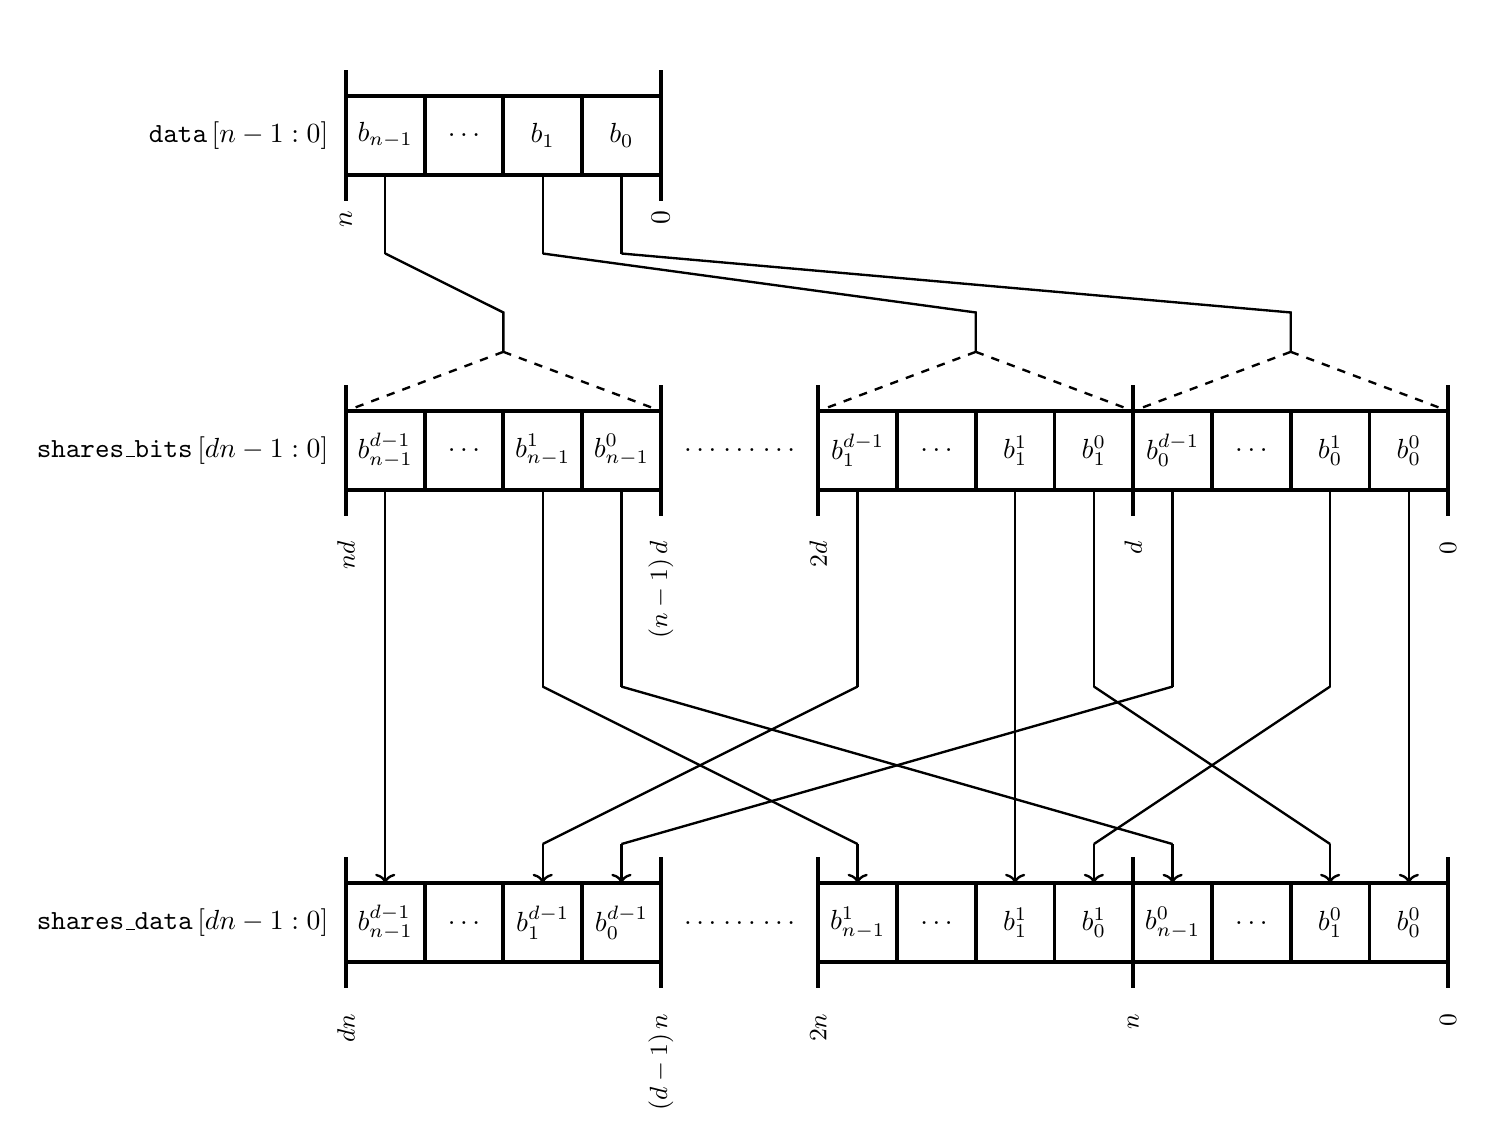
\begin{tikzpicture}
            %% Bus encoding 
% #1: style
% #2: id
% #3: loc (of first cell)
% #4: length
% #5: width elem
\newcommand{\vecNode}[5][]{
    % Draw rectangle
    \coordinate (TL) at ($#3 + (-#5/2,#5/2)$);
    \coordinate (BL) at ($#3 + (-#5/2,-#5/2)$);
    \coordinate (TR) at ($(TL) + (#5*#4,0)$);
    \coordinate (BR) at ($(BL) + (#5*#4,0)$);
    \draw [#1] (TL) -- (TR) -- (BR) -- (BL) -- (TL);
    \foreach \xi in {1,...,#4}{
        \draw[#1] ($(TL) + (#5*\xi,0)$) -- ($(BL) + (#5*\xi,0)$);
        \node at ($#3+(#5*\xi-#5,0)$) {\ifdebug N\xi \else \fi};
        \node at ($#3+(#5*\xi-#5,0.5*#5)$) {\ifdebug o \else \fi};
        \node at ($#3+(#5*\xi-#5,-0.5*#5)$) {\ifdebug o \else \fi};
        \coordinate (#2/N\xi_N) at ($#3+(#5*\xi-#5,0.5*#5)$) {};
        \coordinate (#2/N\xi_S) at ($#3+(#5*\xi-#5,-0.5*#5)$) {};
        \coordinate (#2/N\xi) at ($#3+(#5*\xi-#5,0)$) {};
    }
    % Generate boundaries nodes
    \coordinate (#2/TL) at (TL);
    \coordinate (#2/BL) at (BL);
    \coordinate (#2/TR) at (TR);
    \coordinate (#2/BR) at (BR);
    \coordinate (#2/top) at ($(TL) + (#4/2,0.75#5)$);
    \coordinate (#2/left) at ($(TL) + (0,-#5/2)$);
    % Debug
    \node at (#2/top) {\ifdebug o \else \fi};
    \node at (#2/left) {\ifdebug o \else \fi};
}

%% Encoded bus
% #1: style
% #2: id
% #3: loc (of more left cell)
% #4: width elem
\newcommand{\sharedBus}[4][]{
    \def\propB{0.33}
    \def\offT{0.2}
    \def\fsize{\small}
    % Coordinate
    \coordinate (dd) at #3;
    \coordinate (d1) at ($(dd)+(6*#4,0)$);
    \coordinate (d0) at ($(dd)+(10*#4,0)$);
    % Draw the 3 vecNode
    \vecNode[#1]{#2/dd}{(dd)}{4}{#4}
    \vecNode[#1]{#2/d1}{(d1)}{4}{#4}
    \vecNode[#1]{#2/d0}{(d0)}{4}{#4}
    % Draw the dots
    \node at ($(dd)+(4*#4,0)$) {$\dots$};
    \node at ($(dd)+(4.5*#4,0)$) {$\dots$};
    \node at ($(dd)+(5*#4,0)$) {$\dots$};
    % Draw the vec bounds
    \draw[#1] ($(#2/dd/TL) + (0,\propB*#4)$) -- ($(#2/dd/BL) - (0,\propB*#4)$);
    \draw[#1] ($(#2/dd/TR) + (0,\propB*#4)$) -- ($(#2/dd/BR) - (0,\propB*#4)$);
    \draw[#1] ($(#2/d1/TL) + (0,\propB*#4)$) -- ($(#2/d1/BL) - (0,\propB*#4)$);
    \draw[#1] ($(#2/d1/TR) + (0,\propB*#4)$) -- ($(#2/d1/BR) - (0,\propB*#4)$);
    \draw[#1] ($(#2/d0/TR) + (0,\propB*#4)$) -- ($(#2/d0/BR) - (0,\propB*#4)$);
    % Draw the bit position
    \node [anchor=east, rotate=90] at ($(#2/dd/BL) - (0,\propB*#4) - (0,\offT)$) {\fsize $dn$};
    \node [anchor=east, rotate=90] at ($(#2/dd/BR) - (0,\propB*#4) - (0,\offT)$) {\fsize $\left(d-1\right)n$};

    \node [anchor=east, rotate=90] at ($(#2/d1/BL) - (0,\propB*#4) - (0,\offT)$) {\fsize $2n$};
    \node [anchor=east, rotate=90] at ($(#2/d1/BR) - (0,\propB*#4) - (0,\offT)$) {\fsize $n$};
    \node [anchor=east, rotate=90] at ($(#2/d0/BR) - (0,\propB*#4) - (0,\offT)$) {\fsize $0$};
    % Draw the bits values
    \node at (#2/dd/N1) {$b_{n-1}^{d-1}$};
    \node at (#2/dd/N2) {$\dots$};
    \node at (#2/dd/N3) {$b_{1}^{d-1}$};
    \node at (#2/dd/N4) {$b_{0}^{d-1}$};

    \node at (#2/d1/N1) {$b_{n-1}^{1}$};
    \node at (#2/d1/N2) {$\dots$};
    \node at (#2/d1/N3) {$b_{1}^{1}$};
    \node at (#2/d1/N4) {$b_{0}^{1}$};

    \node at (#2/d0/N1) {$b_{n-1}^{0}$};
    \node at (#2/d0/N2) {$\dots$};
    \node at (#2/d0/N3) {$b_{1}^{0}$};
    \node at (#2/d0/N4) {$b_{0}^{0}$};
    % Coordinate
    \coordinate (#2/left) at (#2/dd/left);
}

%% Shares figure
% #1: style
% #2: id
% #3: loc (of more left cell)
% #4: width elem
\newcommand{\sharesBits}[4][]{
    \def\propB{0.33}
    \def\offT{0.2}
    \def\fsize{\small}
    % Coordinate
    \coordinate (dd) at #3;
    \coordinate (d1) at ($(dd)+(6*#4,0)$);
    \coordinate (d0) at ($(dd)+(10*#4,0)$);
    % Draw the 3 vecNode
    \vecNode[#1]{#2/dd}{(dd)}{4}{#4}
    \vecNode[#1]{#2/d1}{(d1)}{4}{#4}
    \vecNode[#1]{#2/d0}{(d0)}{4}{#4}
    % Draw the dots
    \node at ($(dd)+(4*#4,0)$) {$\dots$};
    \node at ($(dd)+(4.5*#4,0)$) {$\dots$};
    \node at ($(dd)+(5*#4,0)$) {$\dots$};
    % Draw the vec bounds
    \draw[#1] ($(#2/dd/TL) + (0,\propB*#4)$) -- ($(#2/dd/BL) - (0,\propB*#4)$);
    \draw[#1] ($(#2/dd/TR) + (0,\propB*#4)$) -- ($(#2/dd/BR) - (0,\propB*#4)$);
    \draw[#1] ($(#2/d1/TL) + (0,\propB*#4)$) -- ($(#2/d1/BL) - (0,\propB*#4)$);
    \draw[#1] ($(#2/d1/TR) + (0,\propB*#4)$) -- ($(#2/d1/BR) - (0,\propB*#4)$);
    \draw[#1] ($(#2/d0/TR) + (0,\propB*#4)$) -- ($(#2/d0/BR) - (0,\propB*#4)$);
    % Draw the bit position
    \node [anchor=east, rotate=90]at ($(#2/dd/BL) - (0,\propB*#4) - (0,\offT)$) {\fsize $nd$};
    \node [anchor=east, rotate=90]at ($(#2/dd/BR) - (0,\propB*#4) - (0,\offT)$) {\fsize $\left(n-1\right)d$};

    \node [anchor=east, rotate=90]at ($(#2/d1/BL) - (0,\propB*#4) - (0,\offT)$) {\fsize $2d$};
    \node [anchor=east, rotate=90]at ($(#2/d1/BR) - (0,\propB*#4) - (0,\offT)$) {\fsize $d$};
    \node [anchor=east, rotate=90]at ($(#2/d0/BR) - (0,\propB*#4) - (0,\offT)$) {\fsize $0$};
    %% Draw the bits values
    \node at (#2/dd/N1) {$b_{n-1}^{d-1}$};
    \node at (#2/dd/N2) {$\dots$};
    \node at (#2/dd/N3) {$b_{n-1}^{1}$};
    \node at (#2/dd/N4) {$b_{n-1}^{0}$};

    \node at (#2/d1/N1) {$b_{1}^{d-1}$};
    \node at (#2/d1/N2) {$\dots$};
    \node at (#2/d1/N3) {$b_{1}^{1}$};
    \node at (#2/d1/N4) {$b_{1}^{0}$};

    \node at (#2/d0/N1) {$b_{0}^{d-1}$};
    \node at (#2/d0/N2) {$\dots$};
    \node at (#2/d0/N3) {$b_{0}^{1}$};
    \node at (#2/d0/N4) {$b_{0}^{0}$};
    % Coordinate
    \coordinate (#2/left) at (#2/dd/left);
}

%% unshared bus
% #1: style
% #2: id
% #3: loc (of more left cell)
% #4: width elem
\newcommand{\unshare}[4][]{
    \def\propB{0.33}
    \def\offT{0.2}
    \def\fsize{\small}
    % Draw the vecNode
    \vecNode[#1]{#2/bus}{#3}{4}{#4}
    % Draw he vec bounds
    \draw[#1] ($(#2/bus/TL) + (0,\propB*#4)$) -- ($(#2/bus/BL) - (0,\propB*#4)$);
    \draw[#1] ($(#2/bus/TR) + (0,\propB*#4)$) -- ($(#2/bus/BR) - (0,\propB*#4)$);
    % Draw the bit position
    \node [anchor=east, rotate=90] at ($(#2/bus/BL) - (0,\propB*#4)$) {$n$};
    \node [anchor=east, rotate=90] at ($(#2/bus/BR) - (0,\propB*#4)$) {$0$};
    % Draw bit values
    \node at (#2/bus/N1) {$b_{n-1}$};
    \node at (#2/bus/N2) {$\dots$};
    \node at (#2/bus/N3) {$b_{1}$};
    \node at (#2/bus/N4) {$b_{0}$};
    % Coordinate
    \coordinate (#2/left) at (#2/bus/left);
}

% Configuration
\def\cellW{0.5mm}
\def\arrW{0.3mm}
\def\shT{0.1cm}

% Draw basic vects
\def\scaleW{1}
\sharedBus[line width=\cellW]{shared_bus}{(0,0)}{\scaleW}
\sharesBits[line width=\cellW]{shares_bits}{(0,6)}{\scaleW}
\unshare[line width=\cellW]{unshared_bus}{(0,10)}{\scaleW}

% Draw the connector
\foreach \xi in {1,3,4} {
    % Shared bus connectors
    \coordinate (shared_bus/dd/N\xi_N_C) at ($(shared_bus/dd/N\xi_N)+(0,0.5*\scaleW)$);
    \coordinate (shared_bus/d1/N\xi_N_C) at ($(shared_bus/d1/N\xi_N)+(0,0.5*\scaleW)$);
    \coordinate (shared_bus/d0/N\xi_N_C) at ($(shared_bus/d0/N\xi_N)+(0,0.5*\scaleW)$);
    \draw [<-, line width=\arrW] (shared_bus/dd/N\xi_N) -- (shared_bus/dd/N\xi_N_C);
    \draw [<-, line width=\arrW] (shared_bus/d1/N\xi_N) -- (shared_bus/d1/N\xi_N_C);
    \draw [<-, line width=\arrW] (shared_bus/d0/N\xi_N) -- (shared_bus/d0/N\xi_N_C);
    % Shares bits connectors
    \coordinate (shares_bits/dd/N\xi_S_C) at ($(shares_bits/dd/N\xi_S)-(0,2.5*\scaleW)$);
    \coordinate (shares_bits/d1/N\xi_S_C) at ($(shares_bits/d1/N\xi_S)-(0,2.5*\scaleW)$);
    \coordinate (shares_bits/d0/N\xi_S_C) at ($(shares_bits/d0/N\xi_S)-(0,2.5*\scaleW)$);
    \draw [line width=\arrW] (shares_bits/dd/N\xi_S) -- (shares_bits/dd/N\xi_S_C);
    \draw [line width=\arrW] (shares_bits/d1/N\xi_S) -- (shares_bits/d1/N\xi_S_C);
    \draw [line width=\arrW] (shares_bits/d0/N\xi_S) -- (shares_bits/d0/N\xi_S_C);
    % Unshared bus connector
    \coordinate (unshared_bus/bus/N\xi_S_C) at ($(unshared_bus/bus/N\xi_S)+(0,-1*\scaleW)$);
    \draw [line width=\arrW] (unshared_bus/bus/N\xi_S) -- (unshared_bus/bus/N\xi_S_C);
}

% Draw connextion between busses
% First bit share
\draw [line width=\arrW] (shares_bits/d0/N4_S_C) -- (shared_bus/d0/N4_N_C);
\draw [line width=\arrW] (shares_bits/d0/N3_S_C) -- (shared_bus/d1/N4_N_C);
\draw [line width=\arrW] (shares_bits/d0/N1_S_C) -- (shared_bus/dd/N4_N_C);
% Second bit share
\draw [line width=\arrW] (shares_bits/d1/N4_S_C) -- (shared_bus/d0/N3_N_C);
\draw [line width=\arrW] (shares_bits/d1/N3_S_C) -- (shared_bus/d1/N3_N_C);
\draw [line width=\arrW] (shares_bits/d1/N1_S_C) -- (shared_bus/dd/N3_N_C);
% Last bit share
\draw [line width=\arrW] (shares_bits/dd/N4_S_C) -- (shared_bus/d0/N1_N_C);
\draw [line width=\arrW] (shares_bits/dd/N3_S_C) -- (shared_bus/d1/N1_N_C);
\draw [line width=\arrW] (shares_bits/dd/N1_S_C) -- (shared_bus/dd/N1_N_C);
% Draw unshared bus connector
\draw [line width=\arrW] (unshared_bus/bus/N1_S_C) -- ($(shares_bits/dd/top) + (0,0.5)$) -- (shares_bits/dd/top);
\draw [line width=\arrW] (unshared_bus/bus/N3_S_C) -- ($(shares_bits/d1/top) + (0,0.5)$) -- (shares_bits/d1/top);
\draw [line width=\arrW] (unshared_bus/bus/N4_S_C) -- ($(shares_bits/d0/top) + (0,0.5)$) -- (shares_bits/d0/top);

\draw [line width=\arrW,dashed] (shares_bits/dd/top) -- (shares_bits/dd/TL) (shares_bits/dd/top) -- (shares_bits/dd/TR);
\draw [line width=\arrW,dashed] (shares_bits/d1/top) -- (shares_bits/d1/TL) (shares_bits/d1/top) -- (shares_bits/d1/TR);
\draw [line width=\arrW,dashed] (shares_bits/d0/top) -- (shares_bits/d0/TL) (shares_bits/d0/top) -- (shares_bits/d0/TR);

% Names of bus
\node [anchor=east,xshift=-\shT] at (unshared_bus/left) {$\texttt{data}\left[ n-1:0\right]$};
\node [anchor=east,xshift=-\shT] at (shares_bits/left) {$\texttt{shares\_bits}\left[ dn-1:0\right]$};
\node [anchor=east,xshift=-\shT] at (shared_bus/left) {$\texttt{shares\_data}\left[ dn-1:0\right]$};

        \end{tikzpicture}
    }
    \caption{Encoding of a shared $n$-bit wide data with $d$ shares.}
    \label{fig:encoding}
\end{figure}

The key and the input data must be fed as uniform sharings (i.e. the sharing is
selected uniformly at random among possible sharings that represent the correct
value). The output data sharing is guaranteed to be uniform.

\section{Core Architecture}
\label{section:architecture}

The top-level architecture of $\topName$ is depicted in Figure~\ref{fig:smaesh_top_module}:
its main components are the AES unit $\topModAES$, the key storage unit $\topModKHOLD$ and the PRNG. Some additional logic
is used to handle the execution/key configuration/re-seed interlocking, as well as units to shuffle
the shares of the masked busses.

\paragraph{Core}
The module $\topModAES$ implements a masked version of the three variants of
the AES algorithm, in encryption or decryption, by serially processing 32-bits
parts of the state and chosen at run-time. The execution is internally
configured by the $\topModKHOLD$ module that forwards the signals
$\portAESModeI$ and $\portAESModeII$ to select another version than the 128-bit
one used by default and the signal $\portAESInverse$ that specifies that the
reverse algorithm must be executed. It runs a single AES execution at a time
and the output produced ($\portAESOutData$) has to be fetched before a new
execution can start. Together with the configuration signals, the shared input ($\portAESInData$) and the shared key
($\portAESInKey$) are fetched at the beginning of a new execution by performing
a simple transaction at the input interface (with $\portAESInValid$ and
$\portAESInReady$).  Similarly, the shared output ($\portAESOutData$) is output
from the core with a dedicated interface (with $\portAESOutValid$ and
$\portAESOutReady$). The signal $\portAESbusy$ is asserted when an execution is
ongoing inside the core.
Finally, the signals $\portAESKSchedOnly$, $\portAESLastKeyColPreValid$, 
$\portAESLastKeyCol$ and $\portAESRndRfValid$ are only used internally together with the key storage module $\topModKHOLD$ in order to perform specific operation 
related to the key management as detailed in the paragraph "Key Holder" below. 

\paragraph{PRNG}
The module $\topModPRNG$ is generating the randomness required by the 
masking scheme. It is the producer on the randomness bus, while $\topModAES$ is
the receiver.

When not re-seeding, it takes only a single cycle to generate the fresh randomness, therefore
at the next cycle after a randomness transaction, new randomness is already available (i.e.,
$\portAESRnd$ carries fresh randomness, and $\portPrngOutValid$ is asserted).
During an encryption, $\topModAES$ needs randomness at all clock cycles, hence
it keeps $\portPrngOutReady$ asserted, and thanks to the high-throughput
capability of the PRNG, a transaction happens on the randomness bus at every
clock cycles ($\portPrngOutValid$ stays asserted).

This high throughput capability is actually relied upon by $\topModAES$: it
needs randomness for security at every cycle during the encryption
and cannot stall once encryption is started.
The signal $\portPrngOutValid$ is de-asserted only when the PRNG has not been
seeded after a reset, or while it is re-seeding.
To ensure that fresh randomness is always available when encrypting, the
interlocking logic prevents the $\topModAES$ from starting an encryption if
$\portPrngOutValid$ is de-asserted, while it prevents $\topModPRNG$ from
starting a re-seed when an encryption is ongoing.
If no encryption is ongoing and $\svrsSeedValid$ is asserted, then a re-seed is
initiated and a transaction on the \texttt{seed} bus occurs at the next cycle
(this is to avoid a combinational dependency $\svrsSeedValid \rightarrow
\svrsSeedReady$, and is achieved by detecting a rising edge on the PRNG
$\portPrngBusy$ signal).

\paragraph{Key holder}
The module $\topModKHOLD$ is in charge of the key management and the
configuration of the executions performed by the core. This module is mainly
keeping the shares values of the long term key and is in charge of refreshing
the latter after each execution of the core. A new key value is configured
serially by performing transactions of 32-bit piece of data on the key
dedicated interface (i.e., $\portKHDataIn$, $\portKHDataInValid$ and
$\portKHDataInReady$). Besides the key value, the key size (i.e., 128, 192 or
256 bits) is configured during the first transaction of a new key configuration
using the signal $\portKHSizeCfg$ (i.e., 0b00 for 128, 0b01 for 192 and 0b11
for 256). Complementarily, the core can be configured to perform decryption by
asserting the signal $\portKHInverse$ during the first transaction. When a key
configuration is ongoing, the signal $\portKHBusy$ is asserted. 

When configured to compute decryption, the module stores a sharing of the last
round key corresponding the key provided. To do so, the key storage unit
controls the $\topModAES$ module in order to perform a dummy encryption upon
the reception of a new key. In particular, the signal $\portKHLastKeyReq$ is
used to start a dummy encryption with module $\topModAES$ during witch the
logic unrelated to the key schedule algorithm is disabled (using signal
$\portAESKSchedOnly$). At the end of the dummy encryption, the signal
$\portAESLastKeyColPreValid$ is asserted and the value of the (shared) last
round key is fetched back using the bus $\portAESLastKeyCol$, by serially
obtaining the shared value of a single column per cycle. In such a case, the
signal $\portKHBusy$ is asserted until the key material of the last round key
have not been recovered by the key storage unit. 

During each standard execution (i.e., execution not related to a key
configuration), the key shares hold by the module $\topModKHOLD$ are refreshed
on-the-fly. This is made possible due to the fact that some part of the fresh
randomness provided through the bus $\portAESRnd$ to the module $\topModAES$ is
not used by the latter during specific cycles of the execution of a round
function. Such cycles are advertised to the key storage unit by asserting the signal
$\portAESRndRfValid$. It results that the key refresh is performed with no latency penalty.  

\paragraph{Arbitrer}
The module $\topModArbitrer$ is used in order to implement the interlocking
logic internal to the core.  In particular, it takes as input the control
signals of the three input streams (i.e., $\svrsKeyValid$, $\svrsKeyReady$,
$\svrsInValid$, $\svrsInReady$, $\svrsSeedValid$ and $\svrsSeedReady$) and
generate the internal control signal that drive the modules $\topModAES$,
$\topModKHOLD$ and $\topModPRNG$ according to the precedence rules detailled in
Section~\ref{section:core_usage}. 

\paragraph{Share shuffling}
The modules $\texttt{shares2shbus}$ and $\texttt{shbus2shares}$ are simple wire
shuffling that ``transpose'' the encoding of the shared data.
More precisely, the encoding of a sharing inside $\topModAES$
is $\texttt{shares\_data\_inner}\left[ ni+j\right] = b_j^i$ unlike the more
intuitive external representation $\texttt{shares\_data}\left[ ni+j\right] =
b_i^j$ described in Section~\ref{sec:share_encoding}.
This internal representation is more convenient for the implementation, as it
makes it easier to describe the extraction of masked bits from a masked bus
using Verilog operators.

\begin{figure}
    \centering
    \resizebox{\textwidth}{!}{
        \begin{tikzpicture}
            
% Global config
\def\fsIO{\Large}
\def\fontS{\Large}
\def\sizeB{0.9mm}
\def\sizeW{0.4mm}
\def\portOff{0.5}


%\debugtrue

\def\Rad{5pt}
\def\dotRad{0.10}

\tikzset{
dot/.style = {circle, fill, minimum size=#1,
              inner sep=0pt, outer sep=0pt},
dot/.default = 6pt % size of the circle diameter 
}

% W internal port macro with annotation
% #1 style
% #2 id
% #3 loc
% #4 text
\def\yshw{3mm}
\def\xshw{2mm}
\newcommand{\portW}[4][]{
    \node [dot=\Rad] (ncirc) at (#3) {};
    \node [#1,anchor=west,yshift=\yshw] at (#3) {#4};
    \coordinate (#2) at (ncirc.west);
    \coordinate (#2/m) at (ncirc.east);
}
% E internal port macro with annotation
% #1 style
% #2 id
% #3 loc
% #4 text
\newcommand{\portE}[4][]{
    \node [dot=\Rad] (ncirc) at (#3) {};
    \node [#1,anchor=east,yshift=\yshw] at (#3) {#4};
    \coordinate (#2) at (ncirc.east);
    \coordinate (#2/m) at (ncirc.west);
}
% S internal port macro with annotation
% #1 style
% #2 id
% #3 loc
% #4 text
\newcommand{\portS}[4][]{
    \node [dot=\Rad] (ncirc) at (#3) {};
    \node [#1,anchor=east,xshift=\yshw,rotate=270] at (#3) {#4};
    \coordinate (#2) at (ncirc.south);
    \coordinate (#2/m) at (ncirc.north);
}
%%%%%% TOP arrow
\def\awidth{0.4mm}
\def\xarr{2cm}
% W arrow port macro
% #1 port connected
\newcommand{\arrW}[2][]{
    \draw [#1,line width = \awidth] ($(#2)+(-\xarr,0)$) -- (#2);
}
% E arrow port macro
% #1 port connected
\newcommand{\arrE}[2][]{
    \draw [#1,line width = \awidth] (#2) -- ++(\xarr,0);
}

% AES bloc
% #1: id
% #2: pos TR
\newcommand{\blocAES}[2]{
    %% Draw the rectangle
    \rectangleC[line width = 0.6mm]{box}{#2}{($ #2 + (-10,-20)$)}{19}{19}{1}{3};
    \draw node[rectangle,draw,line width=0.6mm,anchor=north west] at (box/TL) {\fontS \topModAES};
    %% Draw the IO ports
    % Draw W
    \portW{#1/in_last_key_col}{box/W2}{\fontS \portAESLastKeyCol}
    \portW{#1/in_last_key_col_pre_valid}{box/W3}{\fontS \portAESLastKeyColPreValid}
    \portW{#1/rnd_rfrsh_valid}{box/W4}{\fontS \portAESRndRfValid}
    \portW{#1/mode_192}{box/W5}{\fontS \portAESModeI}
    \portW{#1/mode_256}{box/W6}{\fontS \portAESModeII}
    \portW{#1/inverse}{box/W7}{\fontS \portAESInverse}
    \portW{#1/key_sched_only}{box/W9}{\fontS \portAESKSchedOnly}
    \portW{#1/in_key}{box/W10}{\fontS \portAESInKey}

    \portW{#1/in_valid}{box/W16}{\fontS \portAESInValid}
    \portW{#1/in_ready}{box/W17}{\fontS \portAESInReady}
    \portW{#1/in_data}{box/W18}{\fontS \portAESInData}
    \portW{#1/busy}{box/W19}{\fontS \portAESbusy}
    % Draw E
    \portE{#1/out_valid}{box/E2}{\fontS \portAESOutValid}
    \portE{#1/out_ready}{box/E3}{\fontS \portAESOutReady}
    \portE{#1/out_data}{box/E4}{\fontS \portAESOutData}
    % Draw S
    \portS{#1/rnd_ready}{box/S2}{\fontS \portAESRndReady}
    \portS{#1/rnd}{box/S3}{\fontS \portAESRnd}
    % Generate coordinate
    \coordinate (#1/center) at #2;
}

% PRNG bloc
% #1: id
% #2: pos TR
\newcommand{\blocPRNG}[2]{
    %% Draw the rectangle
    \rectangleC[line width = 0.6mm]{box}{#2}{($ #2 + (-7,-5)$)}{4}{4}{1}{1};
    \draw node[rectangle,draw,line width=0.6mm,anchor=north west] at (box/TL) {\fontS \topModPRNG};
    %% Internal coordinate
    \coordinate (#1/TR) at (box/TR);
    %% Draw the IO ports
    % Draw W 
    \portW{#1/start_reseed}{box/W2}{\fontS \portPrngStartReseed}
    \portW{#1/in_seed}{box/W3}{\fontS \portPrngSeed}
    \portW{#1/busy}{box/W4}{\fontS \portPrngBusy}
    % Draw E
    \portE{#1/out_valid}{box/E2}{\fontS \portPrngOutValid}
    \portE{#1/out_ready}{box/E3}{\fontS \portPrngOutReady}
    \portE{#1/out_rnd}{box/E4}{\fontS \portPrngOutRnd}
}


% Kunit bloc
% #1: id
% #2: pos TR
\newcommand{\blocKU}[2]{
    %% Draw the rectangle
    \rectangleC[line width = 0.6mm]{box}{#2}{($ #2 + (-11,-18)$)}{17}{17}{1}{5};
    \draw node[rectangle,draw,line width=0.6mm,anchor=north west] at (box/TL) {\fontS \topModKHOLD};
    %% Draw the IO ports
    % Draw E
    \portE{#1/out_last_key_col}{box/E2}{\fontS \portKHLastKeyCol}
    \portE{#1/out_last_key_col_pre_valid}{box/E3}{\fontS \portKHLastKeyColPreValid}
    \portE{#1/rnd_in_valid}{box/E4}{\fontS \portKHRndInValid}
    \portE{#1/mode_192}{box/E5}{\fontS \portKHModeI}
    \portE{#1/mode_256}{box/E6}{\fontS \portKHModeII}
    \portE{#1/mode_inverse}{box/E7}{\fontS \portKHInverse}
    \portE{#1/last_key_required}{box/E9}{\fontS \portKHLastKeyReq}
    \portE{#1/sh_data_out}{box/E10}{\fontS \portKHDataOut}
    \portE{#1/aes_busy}{box/E11}{\fontS \portKHAESbusy}
    % Draw S
    \portS{#1/rnd_rfrsh}{box/S1}{\fontS \portKHRndIn}
    % Draw W
    \portW{#1/data_in}{box/W2}{\fontS \portKHDataIn}
    \portW{#1/in_key_size_cfg}{box/W3}{\fontS \portKHSizeCfg}
    \portW{#1/in_mode_inverse}{box/W4}{\fontS \portKHInInverse}
    \portW{#1/start_fetch}{box/W5}{\fontS \portKHStartFetch}
    \portW{#1/data_in_valid}{box/W6}{\fontS \portKHDataInValid}
    \portW{#1/data_in_ready}{box/W7}{\fontS \portKHDataInReady}
    \portW{#1/busy}{box/W11}{\fontS \portKHBusy}
}


% Arbitrer bloc
% #1: id
% #2: pos TR
\newcommand{\blocArbitrer}[2]{
    %% Draw the rectangle
    \rectangleC[line width = 0.6mm]{box}{#2}{($ #2 + (-10,-15)$)}{14}{14}{1}{1};
    \draw node[rectangle,draw,line width=0.6mm,anchor=north west] at (box/TL) {\fontS \topModArbitrer};
    %% Draw the IO ports
    % Draw W
    \portW{#1/in_key_valid}{box/W2}{\fontS \svrsKeyValid}
    \portW{#1/in_key_ready}{box/W3}{\fontS \svrsKeyReady}
    \portW{#1/in_data_valid}{box/W6}{\fontS \svrsInValid}
    \portW{#1/in_data_ready}{box/W7}{\fontS \svrsInReady}
    \portW{#1/in_seed_valid}{box/W9}{\fontS \svrsSeedValid}
    \portW{#1/in_seed_ready}{box/W10}{\fontS \svrsSeedReady}
    % Draw E
    \portE{#1/KSU_start_fetch}{box/E2}{\fontS \portArbKSUStartFetch}
    \portE{#1/KSU_in_ready}{box/E3}{\fontS \portArbKSUReady}
    \portE{#1/KSU_busy}{box/E4}{\fontS \portArbKHBusy}
    \portE{#1/KSU_lkey_req}{box/E5}{\fontS \portArbKSULastKeyReq}
    \portE{#1/KSU_valid_in}{box/E6}{\fontS \portArbKSUValidIn}
    \portE{#1/aes_valid_in}{box/E7}{\fontS \portArbAESValidIn}
    \portE{#1/aes_in_ready}{box/E8}{\fontS \portArbAESReady}
    \portE{#1/aes_busy}{box/E9}{\fontS \portArbAESBusy}
    \portE{#1/prng_busy}{box/E11}{\fontS \portArbPrngBusy}
    \portE{#1/prng_seeded}{box/E12}{\fontS \portArbPrngSeeded}
    \portE{#1/prng_start_reseed}{box/E13}{\fontS \portArbPrngStartReseed}


}

%%% Draw AES block
\blocAES{aesModule}{(0,0)}

%%% Draw PRNG
\blocPRNG{prngMod}{(-18,-21)}

%%% Draw arbitrer
\blocArbitrer{arbitrer}{(-30,-5)}

%%% Draw Kholder
\blocKU{keyHolder}{(-15,0)}


%%% Draw the and at the input of the inverse signal to AES
\node[and port, anchor=in 1,xshift=1cm](and2_aes_inverse) at (keyHolder/mode_inverse){};
\node at (and2_aes_inverse.bin 2) [ocirc, left]{};

%%%%%%% DRAW INTERNAL connexion

%% KS <-> AES
\draw [line width=\sizeW, ->] (aesModule/in_last_key_col) -- (keyHolder/out_last_key_col);
\draw [line width=\sizeW, ->] (aesModule/in_last_key_col_pre_valid) -- (keyHolder/out_last_key_col_pre_valid);
\draw [line width=\sizeW, ->] (aesModule/rnd_rfrsh_valid) -- (keyHolder/rnd_in_valid);
\draw [line width=\sizeW, ->] (keyHolder/mode_192) -- (aesModule/mode_192);
\draw [line width=\sizeW, ->] (keyHolder/mode_256) -- (aesModule/mode_256);
\draw [line width=\sizeW, ->] (keyHolder/mode_inverse) -- (and2_aes_inverse.in 1);
\draw [line width=\sizeW, ->] (and2_aes_inverse.out) -- ++(0.5,0) |- (aesModule/inverse);
\draw [line width=\sizeW, ->] (keyHolder/last_key_required) --++(0.7,0) |- (and2_aes_inverse.in 2);
\draw [line width=\sizeW, ->] (keyHolder/last_key_required) -- (aesModule/key_sched_only);
\draw [line width=\sizeW, ->] (keyHolder/sh_data_out) -- (aesModule/in_key);
\draw [line width=\sizeW, ->] (aesModule/busy) -- ++(-0.7,0) |- (keyHolder/aes_busy);

%% Output
\node[xshift=5cm, anchor=west,color=colorOUT] (svrs_out_data_valid) at (aesModule/out_valid) {$\svrsOutValid$};
\path let \p1=(svrs_out_data_valid.west),\p2=(aesModule/out_ready) in coordinate (west_svrs_out_data_ready) at (\x1,\y2);
\node [anchor=west,color=colorOUT] (svrs_out_data_ready) at (west_svrs_out_data_ready) {$\svrsOutReady$};
\path let \p1=(svrs_out_data_valid.west),\p2=(aesModule/out_data) in coordinate (west_svrs_out_data) at (\x1,\y2);
\node [anchor=west,color=colorOUT] (svrs_out_data) at (west_svrs_out_data) {$\svrsOutData$};
\node [draw,rectangle,xshift=1cm,anchor=west] (shares2sh_out) at (aesModule/out_data) {\texttt{shbus2shares}};

% randomness
\draw [line width=\sizeW, ->] (aesModule/rnd_ready) |- (prngMod/out_ready);
\draw [line width=\sizeW, ->] (prngMod/out_rnd) -| (aesModule/rnd);
\coordinate (loc_rnd_to_KU_tmp) at ($(prngMod/TR)+(\portOff,\portOff)$);
\path let \p1=(keyHolder/rnd_rfrsh), \p2=(prngMod/TR) in coordinate (anchor_rnd_ku) at ($(\x1,\y2)+(0,0.5)$);
\draw [line width=\sizeW, ->] (prngMod/out_rnd) -- ++(\portOff,0) |- (anchor_rnd_ku) -- (keyHolder/rnd_rfrsh);
% output
\draw [line width=\sizeW, ->, color=colorOUT] (aesModule/out_valid) |- (svrs_out_data_valid.west);
\draw [line width=\sizeW, ->, color=colorOUT] (aesModule/out_ready) |- (svrs_out_data_ready.west);
\draw [line width=\sizeW, color=colorOUT] (aesModule/out_data) -- (shares2sh_out.west);
\draw [line width=\sizeW, ->, color=colorOUT] (shares2sh_out.east) -- (svrs_out_data.west);


%% AES valid in structure
%\draw [line width=\sizeW, ->] (keyHolder/last_key_required) -- ++(0.7,0) |- ($(and2_aes_valid_in_I.in 1)+(-1.5,1)$) |- (and2_aes_valid_in_II.in 1);
%\draw [fill=black] ($(keyHolder/last_key_required)+(0.7,0)$) circle (\dotRad);
%\draw [line width=\sizeW, ->] (aesModule/busy) -| ($(and2_aes_valid_in_II.in 2)+(-0.5,0)$) -- (and2_aes_valid_in_II.in 2);
%\draw [line width=\sizeW, ->] (keyHolder/busy) -- ++(-0.5,0) |- (and2_aes_valid_in_I.in 1);
%\draw [line width=\sizeW, ->] (and2_aes_valid_in_I.out) |- (or2_aes_valid_in.in 1);
%\draw [line width=\sizeW, ->] (and2_aes_valid_in_II.out) |- (or2_aes_valid_in.in 2);
%\draw [line width=\sizeW, ->] (or2_aes_valid_in.out) |- (and2_aes_valid_in.in 1);
%\draw [line width=\sizeW, ->] (and2_aes_valid_in.out) |- (aesModule/in_valid);
%\draw [line width=\sizeW, <-] (and2_aes_valid_in.in 2) -- ++(-0.5,0) |- (prngMod/out_valid);

%% in ready structure 
%\draw [line width=\sizeW, ->] (keyHolder/last_key_required) -- ++(0.7,0) |- ($(and2_aes_valid_in_I.in 1)+(-1.5,1)$) |- (and4_ready_in.in 3);
%\draw [line width=\sizeW, ->] (keyHolder/busy) -- ++(-0.5,0) |- (and4_ready_in.in 4);
%\draw [line width=\sizeW, ->] (and2_aes_valid_in.in 2) -- ++(-0.5,0) |- (and4_ready_in.in 1);
%\draw [line width=\sizeW, ->] (aesModule/in_ready) -- (and4_ready_in.in 2);

%%% DRAW PORT
%% Data in
%\node [xshift=-22cm,anchor=east,color=colorIN] (svrs_in_data_valid) at (and2_aes_valid_in_I.in 2) {$\svrsInDataValid$};
%\path let \p1=(svrs_in_data_valid.east),\p2=(and4_ready_in.out) in coordinate (east_svrs_in_data_ready) at (\x1,\y2);
%\node [anchor=east,color=colorIN] (svrs_in_data_ready) at (east_svrs_in_data_ready) {$\svrsInDataReady$};
%\path let \p1=(svrs_in_data_valid.east),\p2=(aesModule/in_data) in coordinate (east_svrs_in_data) at (\x1,\y2);
%\node [anchor=east,color=colorIN] (svrs_in_data) at (east_svrs_in_data) {$\svrsInData$};
%% KEY
%\path let \p1=(svrs_in_data_valid.east),\p2=(keyHolder/data_in_valid) in coordinate (east_svrs_key_valid) at (\x1,\y2);
%\node [anchor=east,color=colorKEY] (svrs_key_valid) at (east_svrs_key_valid) {$\svrsKeyValid$};
%\path let \p1=(svrs_in_data_valid.east),\p2=(keyHolder/data_in_ready) in coordinate (east_svrs_key_ready) at (\x1,\y2);
%\node [anchor=east,color=colorKEY] (svrs_key_ready) at (east_svrs_key_ready) {$\svrsKeyReady$};
%\path let \p1=(svrs_in_data_valid.east),\p2=(keyHolder/data_in) in coordinate (east_svrs_key_data) at (\x1,\y2);
%\node [anchor=east,color=colorKEY] (svrs_key_data) at (east_svrs_key_data) {$\svrsKey$};
%\path let \p1=(svrs_in_data_valid.east),\p2=(keyHolder/in_key_size_cfg) in coordinate (east_svrs_key_size_cfg) at (\x1,\y2);
%\node [anchor=east,color=colorKEY] (svrs_key_size_cfg) at (east_svrs_key_size_cfg) {$\svrsKeySizeCfg$};
%\path let \p1=(svrs_in_data_valid.east),\p2=(keyHolder/in_mode_inverse) in coordinate (east_svrs_mode_inverse) at (\x1,\y2);
%\node [anchor=east,color=colorKEY] (svrs_mode_inverse) at (east_svrs_mode_inverse) {$\svrsKeyModeInverse$};
%% REseed
%\path let \p1=(svrs_in_data_valid.east),\p2=(and4_start_reseed.in 4) in coordinate (east_svrs_reseed_in) at (\x1,\y2);
%\node [anchor=east,color=colorSEED] (svrs_seed_valid) at (east_svrs_reseed_in) {$\svrsSeedValid$};
%\path let \p1=(svrs_in_data_valid.east),\p2=(prngMod/in_seed) in coordinate (east_svrs_seed_in) at (\x1,\y2);
%\node [anchor=east,color=colorSEED] (svrs_seed_in) at (east_svrs_seed_in) {$\svrsSeed$};
%\path let \p1=(svrs_in_data_valid.east),\p2=(prngMod/busy) in coordinate (east_svrs_seed_ready) at (\x1,\y2);
%\node [anchor=east,color=colorSEED] (svrs_seed_ready) at (east_svrs_seed_ready) {$\svrsSeedReady$};

%%% Draw the encoding node
%% node for the input
%\path let \p1=(and4_ready_in.in 1), \p2=(svrs_in_data) in coordinate (shares2sh_in_loc) at (\x1, \y2);
%\node [draw,rectangle] (shares2sh_in) at (shares2sh_in_loc) {\texttt{shares2shbus}};

%% Draw the remaining connexions
%% Key ports
% key valid
%\draw [line width=\sizeW, ->, color=colorKEY] (svrs_key_valid.east) -- ++(\portOff+1, 0) |- (and5_start_fetch.in 5);
%\draw [line width=\sizeW, ->, color=colorKEY] (svrs_key_valid.east) -- (keyHolder/data_in_valid);
% key others
%\draw [line width=\sizeW, ->, color=colorKEY] (keyHolder/data_in_ready) -- (svrs_key_ready.east);
%\draw [line width=\sizeW, ->, color=colorKEY] (svrs_key_data.east) -- (keyHolder/data_in);
%\draw [line width=\sizeW, ->, color=colorKEY] (svrs_key_size_cfg.east) -- (keyHolder/in_key_size_cfg);
%\draw [line width=\sizeW, ->, color=colorKEY] (svrs_mode_inverse) -- (keyHolder/in_mode_inverse);
% data in
%\draw [line width=\sizeW, ->, color=colorIN] (svrs_in_data_valid) -- (and2_aes_valid_in_I.in 2);
%\draw [line width=\sizeW, ->, color=colorIN] (svrs_in_data_valid.east) -- ++(\portOff+1.5, 0) |- (and5_start_fetch.in 1);
%\draw [line width=\sizeW, ->, color=colorIN] (svrs_in_data_valid.east) -- ++(\portOff+1.5, 0) |- (and4_start_reseed.in 3);
%\draw [fill=colorIN] ($(svrs_in_data_valid.east)+(\portOff+1.5,0)$) circle (\dotRad);
%\draw [line width=\sizeW, ->, color=colorIN] (and4_ready_in.out) -- (svrs_in_data_ready);
%\draw [line width=\sizeW, ->, color=colorIN] (svrs_in_data) -- (shares2sh_in.west);
%\draw [line width=\sizeW, ->, color=colorIN] (shares2sh_in.east) -- (aesModule/in_data);
% seed
%\draw [line width=\sizeW, ->, color=colorSEED] (svrs_seed_valid.east) -- (and4_start_reseed.in 4);
%\draw [line width=\sizeW, ->, color=colorSEED] (svrs_seed_valid.east) -- ++(\portOff+2, 0) |- (and5_start_fetch.in 2);
%\draw [line width=\sizeW, ->, color=colorSEED] (svrs_seed_in.east) -- (prngMod/in_seed);
%\coordinate (loc_seed_ready_tmp) at ($(and2_seed_ready.out)+(0.5,-2)$);
%\draw [line width=\sizeW, color=colorSEED] (and2_seed_ready.out) -| (loc_seed_ready_tmp);
%\draw [line width=\sizeW, color=colorSEED, <-] (svrs_seed_ready.east) -- ++(\portOff,0) |- (loc_seed_ready_tmp);
% KSU busy
%\coordinate (anchor_ksu_busy) at ($(and4_ready_in.in 4)+(3,0)$);
%\draw [line width=\sizeW, ->] (anchor_ksu_busy) |- (and4_start_reseed.in 1);
% aes busy
%\path let \p1=(anchor_ksu_busy), \p2=(aesModule/busy) in coordinate (anchor_aes_busy) at ($(\x1,\y2)+(-0.5,0)$);
%\draw [line width=\sizeW] (aesModule/busy) -- (anchor_aes_busy);
%\draw [line width=\sizeW,->] (anchor_aes_busy) |- (and4_start_reseed.in 2);
%\draw [line width=\sizeW,->] (anchor_aes_busy) |- (and5_start_fetch.in 4);
% PRNG busy
%\path let \p1=(anchor_aes_busy), \p2=(prngMod/busy) in coordinate (anchor_prng_busy) at ($(\x1,\y2)+(-0.5,0)$);
%\draw [line width=\sizeW,->] (anchor_prng_busy) |- (and5_start_fetch.in 3);

%% DRAw output of and5
%\draw [line width=\sizeW,->] (and4_start_reseed.out) -- (prngMod/start_reseed);
%\draw [line width=\sizeW,->] (and5_start_fetch.out) -- (keyHolder/start_fetch);





        \end{tikzpicture}
    }
    \caption{Global architecture of the module \topName.}
    \label{fig:smaesh_top_module}
\end{figure}

\subsection{Masked AES Core Architecture} 
\label{section:masked_aes_core_arhcitecture}

\begin{figure}
    \centering
    \resizebox{\textwidth}{!}{
        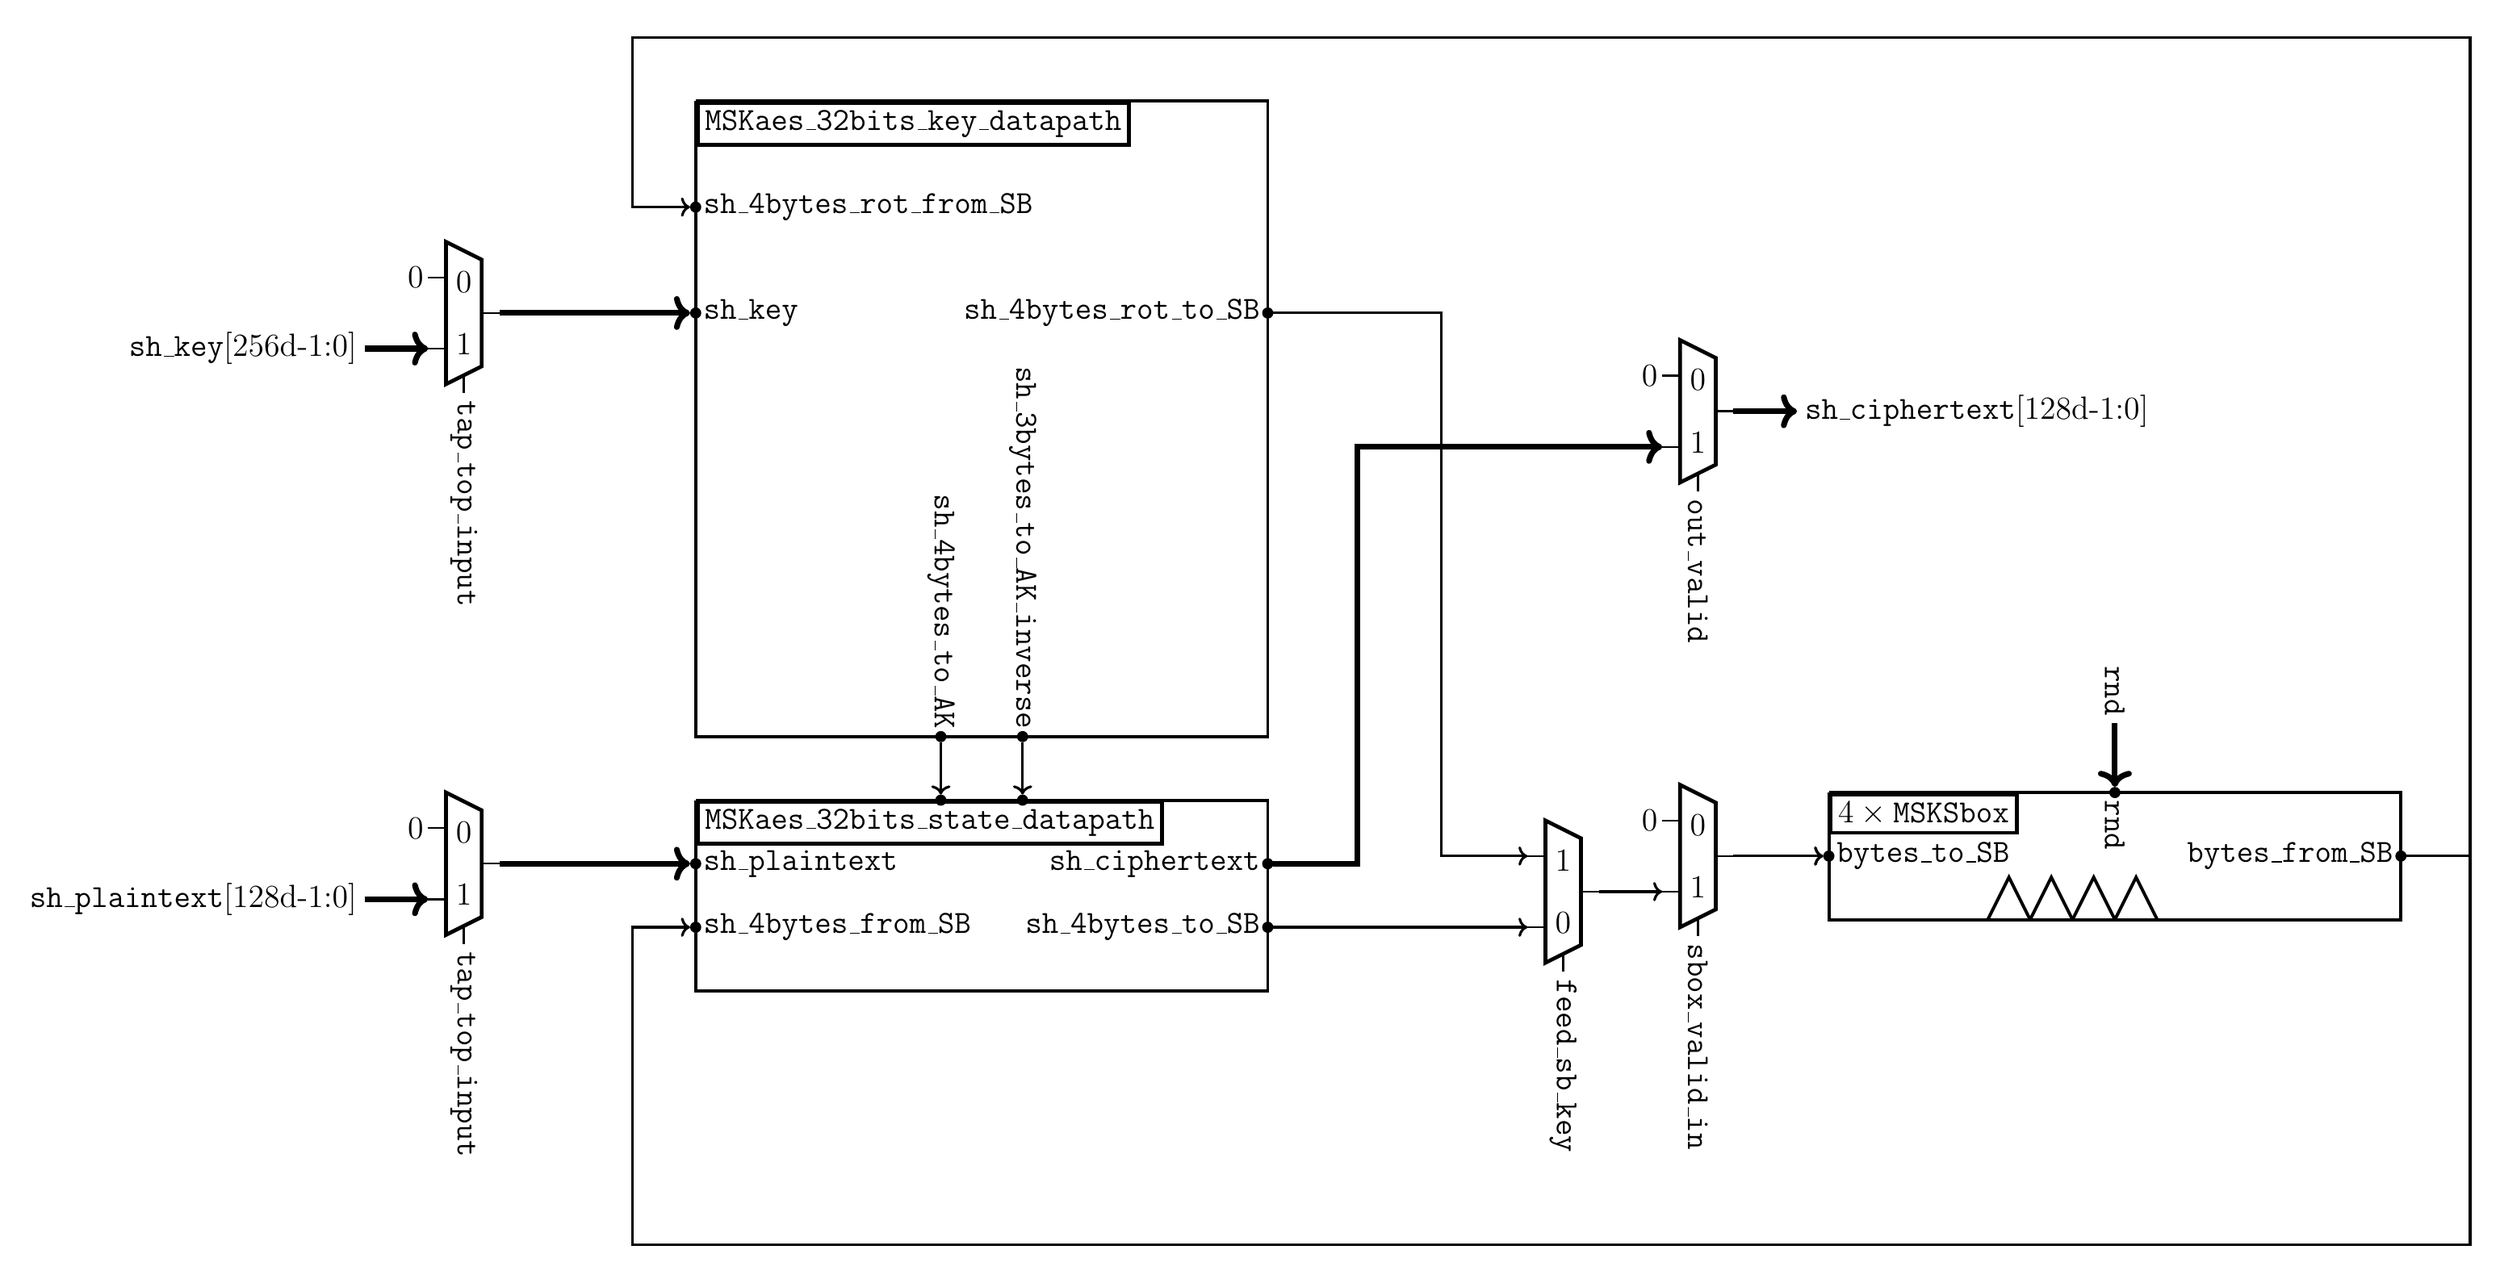
\begin{tikzpicture}
            % define a mux
\tikzset{mux/.style={muxdemux,muxdemux def={Lh=4, NL=2, Rh=3,NB=1,w=1}}}

%%%% Config 
\def\blocLw{0.5mm}
\def\ctLw{0.3mm}
\def\wireLw{0.4mm}
\def\borderLw{0.7mm}

\def\fsizeTop{\Large}
\def\fontS{\Large}
\def\fontCtrl{\Large}

\def\spacexMuxGate{3cm}
\def\xshMuxToSB{4cm}
\def\xshSboxOut{1cm}

\def\sizeB{0.9mm}

% Dot use for Ports
\def\Rad{5pt}
\tikzset{
dot/.style = {circle, fill, minimum size=#1,
              inner sep=0pt, outer sep=0pt},
dot/.default = 6pt % size of the circle diameter 
}

% W internal port macro with annotation
% #1 style
% #2 id
% #3 loc
% #4 text
\def\yshw{3mm}
\def\xshw{2mm}
\newcommand{\portW}[4][]{
    \node [dot=\Rad] (ncirc) at (#3) {};
    \node [#1,anchor=west] at (#3) {#4};
    \coordinate (#2) at (ncirc.west);
    \coordinate (#2/m) at (ncirc.east);
}
% E internal port macro with annotation
% #1 style
% #2 id
% #3 loc
% #4 text
\newcommand{\portE}[4][]{
    \node [dot=\Rad] (ncirc) at (#3) {};
    \node [#1,anchor=east] at (#3) {#4};
    \coordinate (#2) at (ncirc.east);
    \coordinate (#2/m) at (ncirc.west);
}
% S internal port macro with annotation
% #1 style
% #2 id
% #3 loc
% #4 text
\newcommand{\portS}[4][]{
    \node [dot=\Rad] (ncirc) at (#3) {};
    \node [#1,anchor=east,rotate=270] at (#3) {#4};
    \coordinate (#2) at (ncirc.south);
    \coordinate (#2/m) at (ncirc.north);
}
% N internal port macro with annotation
% #1 style
% #2 id
% #3 loc
% #4 text
\newcommand{\portN}[4][]{
    \node [dot=\Rad] (ncirc) at (#3) {};
    \node [#1,anchor=west,rotate=270] at (#3) {#4};
    \coordinate (#2) at (ncirc.north);
    \coordinate (#2/m) at (ncirc.south);
}

%%%%%% TOP arrow
\def\awidth{0.4mm}
\def\xarr{2cm}
% W arrow port macro
% #1 port connected
\newcommand{\arrW}[2][]{
    \draw [#1,line width = \awidth] ($(#2)+(-\xarr,0)$) -- (#2);
}
% E arrow port macro
% #1 port connected
\newcommand{\arrE}[2][]{
    \draw [#1,line width = \awidth] (#2) -- ++(\xarr,0);
}
% S arrow port macro
% #1 port connected
\newcommand{\arrS}[2][]{
    \draw [#1,line width = \awidth] (#2) -- ++(0,-\xarr);
}

%% Macro for the ctrl signals of the mux2
% 1: mux_id
% 2: control sig
% 3: top value
% 4: bottom value
\newcommand{\muxCtrl}[4]{
    \node[anchor=west,rotate=270] at (#1.bpin 1) {\fontCtrl #2};
    \node at (#1.center up) {\fontCtrl #3};
    \node at (#1.center down) {\fontCtrl #4};
}

%% Sbox layer
% #1: draw param
% #2: id
% #3: center loc
\newcommand{\sboxLayer}[3][]{
    % Config
    \def\sbWidth{9}
    \def\sbHeight{2}
    % Draw the Basic rectangle 
    \rectangle[#1]{rec}{#3}{\sbWidth}{\sbHeight}{1}{1}{1}{0}
    \draw node[rectangle,draw,line width=0.6mm,anchor=north west] at (rec/TL) {\fontS $4 \times \modAESsbox$};
    % Draw the pipelie triangles
    \pgfmathsetmacro\trigBase{\sbHeight/3}
    \foreach \xi in {0,...,3}{
        \coordinate (trigCB) at ($(rec/BL) + (0.5*\sbWidth+-2.5*\trigBase,0) + (\xi*\trigBase,0)$);        
        \coordinate (trigC0) at ($(trigCB) + (-\trigBase/2,0)$);
        \coordinate (trigC1) at ($(trigCB) + (0,\trigBase)$);
        \coordinate (trigC2) at ($(trigCB) + (\trigBase/2,0)$);
        \draw [#1] (trigC0) -- (trigC1) --(trigC2);
    }
    % Create ports
    \portW{#2/in}{rec/W1}{\fontS \AESsboxIn}
    \portE{#2/out}{rec/E1}{\fontS \AESsboxOut}
    \portN{#2/rnd}{rec/N1}{\fontS \AESsboxRnd}
}

%% Datapath module for the state
% #1: draw param
% #2: id
% #3: center loc
\newcommand{\dpState}[3][]{
    % Draw rect
    \rectangle[#1]{rec}{#3}{9}{3}{2}{2}{6}{0}
    \draw node[rectangle,draw,line width=0.6mm,anchor=north west] at (rec/TL) {\fontS \modAESdpState};
    % Draw ports
    \portW{#2/plaintext}{rec/W1}{\fontS \AESdpStatePlaintext}
    \portW{#2/from_SB}{rec/W2}{\fontS \AESdpStateFromSB}
    \portN{#2/from_key}{rec/N3}{}%\AESdpStateFromKey
    \portN{#2/from_key_inverse}{rec/N4}{}%\AESdpStateFromKey
    \portE{#2/to_SB}{rec/E2}{\fontS \AESdpStateToSB}
    \portE{#2/ciphertext}{rec/E1}{\fontS \AESdpStateCiphertext}
    % Generating coordinate
    \coordinate (#2/BL) at (rec/BL);
    \coordinate (#2/north) at (rec/north);
}

%% Datapath module for the key
% #1: draw param
% #2: id
% #3: center loc
\newcommand{\dpKey}[3][]{
    % Draw rect
    \rectangle[#1]{rec}{#3}{9}{10}{5}{2}{0}{6}
    \draw node[rectangle,draw,line width=0.6mm,anchor=north west] at (rec/TL) {\fontS \modAESdpKey};
    % Draw ports
    \portW{#2/key}{rec/W2}{\fontS \AESdpKeyKey}
    \portE{#2/to_SB}{rec/E1}{\fontS \AESdpKeyToSB}
    \portW{#2/from_SB}{rec/W1}{\fontS \AESdpKeyFromSB}
    \portS{#2/to_AK}{rec/S3}{\fontS \AESdpKeyToAK}
    \portS{#2/to_AK_inv}{rec/S4}{\fontS \AESdpKeyToAKInverse}
    % Draw generating coordinate
    \coordinate (#2/TL) at (rec/TL);
    \coordinate (#2/south) at (rec/south);
}

%%%% Draw main drawing
\coordinate (locdpState) at (0,0);

%%% Draw dpState + muxes to SB + input muxes
\dpState[line width=\blocLw]{dpState}{(locdpState)}
\node[mux,line width=\ctLw,anchor=lpin 2, xshift=\xshMuxToSB] (mux_to_SB) at (dpState/to_SB) {};
\node[mux,line width=\ctLw,anchor=lpin 2, xshift=1cm] (mux_gate_SB) at (mux_to_SB.rpin 1) {};
\node[mux,line width=\ctLw, anchor=rpin 1,yshift=7cm] (mux_gate_cipher) at (mux_gate_SB.rpin 1) {};
\node[mux,line width=\ctLw,anchor=rpin 1,xshift=-\spacexMuxGate] (mux_gate_plain) at (dpState/plaintext) {};

% Ctrl signals
\muxCtrl{mux_to_SB}{\AESsboxFeedKey}{1}{0}
\muxCtrl{mux_gate_SB}{\AESsboxValidIn}{0}{1}
\muxCtrl{mux_gate_cipher}{\portAESOutValid}{0}{1}
\muxCtrl{mux_gate_plain}{\AESFetchIn}{0}{1}

%% Draw Sbox
\sboxLayer[line width=\blocLw]{sbox}{($(mux_gate_SB.rpin 1) + (6,0)$)}

%% Draw dpKey + input mux
\dpKey[line width=\blocLw]{dpKey}{($(dpState/north) + (0,6)$)}
\node[mux,line width=\ctLw,anchor=rpin 1,xshift=-\spacexMuxGate] (mux_gate_key) at (dpKey/key) {};
\muxCtrl{mux_gate_key}{\AESFetchIn}{0}{1}

%% Draw internal wires
\draw [->,line width=\sizeB] (mux_gate_plain.rpin 1) -- ++(1,0) |- (dpState/plaintext);
\draw [->,line width=\sizeB] (mux_gate_key.rpin 1) -- ++(1,0) |- (dpKey/key);
\draw [->,line width=\wireLw] (dpState/to_SB) -- (mux_to_SB.lpin 2);
\draw [->,line width=\wireLw] (mux_to_SB.rpin 1) -- (mux_gate_SB.lpin 2);
\draw [->,line width=\wireLw] (mux_gate_SB.rpin 1) -- (sbox/in);
\draw [->,line width=\wireLw] (mux_gate_SB.rpin 1) -- (sbox/in);
\draw [->,line width=\wireLw] (dpKey/to_SB) -- ++(0.66*\xshMuxToSB,0) |- (mux_to_SB.lpin 1);
\draw [->,line width=\sizeB] (dpState/ciphertext) -- ++(0.33*\xshMuxToSB,0) |- (mux_gate_cipher.lpin 2);
\draw [->,line width=\wireLw] (dpKey/to_AK) -- (dpState/from_key);
\draw [->,line width=\wireLw] (dpKey/to_AK_inv) -- (dpState/from_key_inverse);

%% Draw feedback wires
\coordinate (sboxOut) at ($(sbox/out)+(\xshSboxOut,0)$);
\debugN[sboxOut]{(sboxOut)}

\coordinate (fbdpKey) at ($(dpKey/TL)+(-1,1)$);
\debugN[fbdpKey]{(fbdpKey)}

\coordinate (fbdpState) at ($(dpState/BL)+(-1,-4)$);
\debugN[fbdpKey]{(fbdpState)}

\draw [line width=\wireLw] (sbox/out) -- (sboxOut);
\draw [->, line width=\wireLw] (sboxOut) |- (fbdpKey) |- (dpKey/from_SB);
\draw [->, line width=\wireLw] (sboxOut) |- (fbdpState) |- (dpState/from_SB);

%% Draw the 0
\node [xshift=-0.2cm] at (mux_gate_cipher.lpin 1) {\fontS $0$};
\node [xshift=-0.2cm] at (mux_gate_plain.lpin 1) {\fontS $0$};
\node [xshift=-0.2cm] at (mux_gate_key.lpin 1) {\fontS $0$};
\node [xshift=-0.2cm] at (mux_gate_SB.lpin 1) {\fontS $0$};


%% Draw port
\draw node[rectangle,anchor=east,xshift=-1cm] (top_plaintext) at (mux_gate_plain.lpin 2){\fsizeTop \portAESInPlaintext [128d-1:0]};
\draw node[rectangle,anchor=east,xshift=-1cm] (top_key) at (mux_gate_key.lpin 2){\fsizeTop \portAESInKey [256d-1:0]};
\draw node[rectangle,anchor=west,xshift=1cm] (top_ciphertext) at (mux_gate_cipher.rpin 1){\fsizeTop \portAESOutCipher [128d-1:0]};
\draw node[rectangle,anchor=east,rotate=270,xshift=-1cm] (top_rnd) at (sbox/rnd){\fsizeTop \portAESRnd };

\draw [->,line width = \sizeB] (top_plaintext.east) -- (mux_gate_plain.lpin 2);
\draw [->,line width = \sizeB] (top_key.east) -- (mux_gate_key.lpin 2);
\draw [->,line width = \sizeB] (mux_gate_cipher.rpin 1) -- (top_ciphertext.west);
\draw [->,line width = \sizeB] (top_rnd.east) -- (sbox/rnd);


        \end{tikzpicture}
    }
    \caption{Datapath architecture of the module \topModAES. Wires not in bold are $32d$ bits wide (apart from muxes control signals).}
    \label{fig:aes_glob_arch}
\end{figure}

The module $\topModAES$ is based on the 32-bit masked AES implementation
presented in~\cite{DBLP:conf/cosade/MominCS22}. As shown in
Figure~\ref{fig:aes_glob_arch}, the module is organized around two datapath
blocks performing the operations dedicated to the round computation (denoted
\modAESdpState) and the key scheduling (denoted $\modAESdpKey$). The module
$\modAESsbox$ is shared between the two datapath blocks and implements the
$\SB$ layer for 4 masked bytes. In particular, it is composed of 4~parallel
instances of the masked S-boxes implementation presented
in~\cite{DBLP:journals/tches/CassiersGMMN24} that relies on the representation
presented in~\cite{DBLP:conf/ches/Canright05}.  Each instance implements both
the forward and inverse operation, chosen at run-time using a dedicated control
signal. More into the details, the S-box is composed of three different layers:
a non-linear layer surrounded by a linear layer at input and output. While the
linear layers (both at the input and output) are different for forward and
inverse operation, the (costly) non-linear layer remains the same and can be
shared when performing operations in both ways.  Executing either the forward
or inverse operation is done in practice by using muxes at the input/output
linear layers that forwards the data accordingly to the chosen mode of execution. 

The S-boxes have been generated using COMPRESS, and are thus optimized for a
given amount of shares. The amount of shares implemented in a practical
integration can be modified at synthesis time by changing the generic $d$ at
the top level. However, a mismatch between the amount of shares instantiated
and the amount of shares specified during the S-box generation with COMPRESS
may lead to suboptimal performance (i.e., area). In this
document, we report the results for four different protection levels, namely
$d\in[2,3,4,5]$. If another amount of shares is required, it is advised to
generate an optimal S-box implementation using COMPRESS\footnote{Please refer
    to
    \href{https://github.com/cassiersg/compress_artifact}{https://github.com/cassiersg/compress\_artifact}
for more info}.  Overall, a single S-box instance is organized as a pipeline of 4 stages that
requires 36 random bits (resp. 96, 192 and 300) per execution considering $d=2$
(resp. 3, 4 and 5). The bus $\portAESRnd$ is used to provide the fresh
randomness to the 4~S-boxes instances (randomness is not used anywhere else in
$\topModAES$). 

\subsection{Architecture of the $\modAESdpState$ module}
\label{sec:architecture}

\begin{figure}
    \centering
    \resizebox{\textwidth}{!}{
        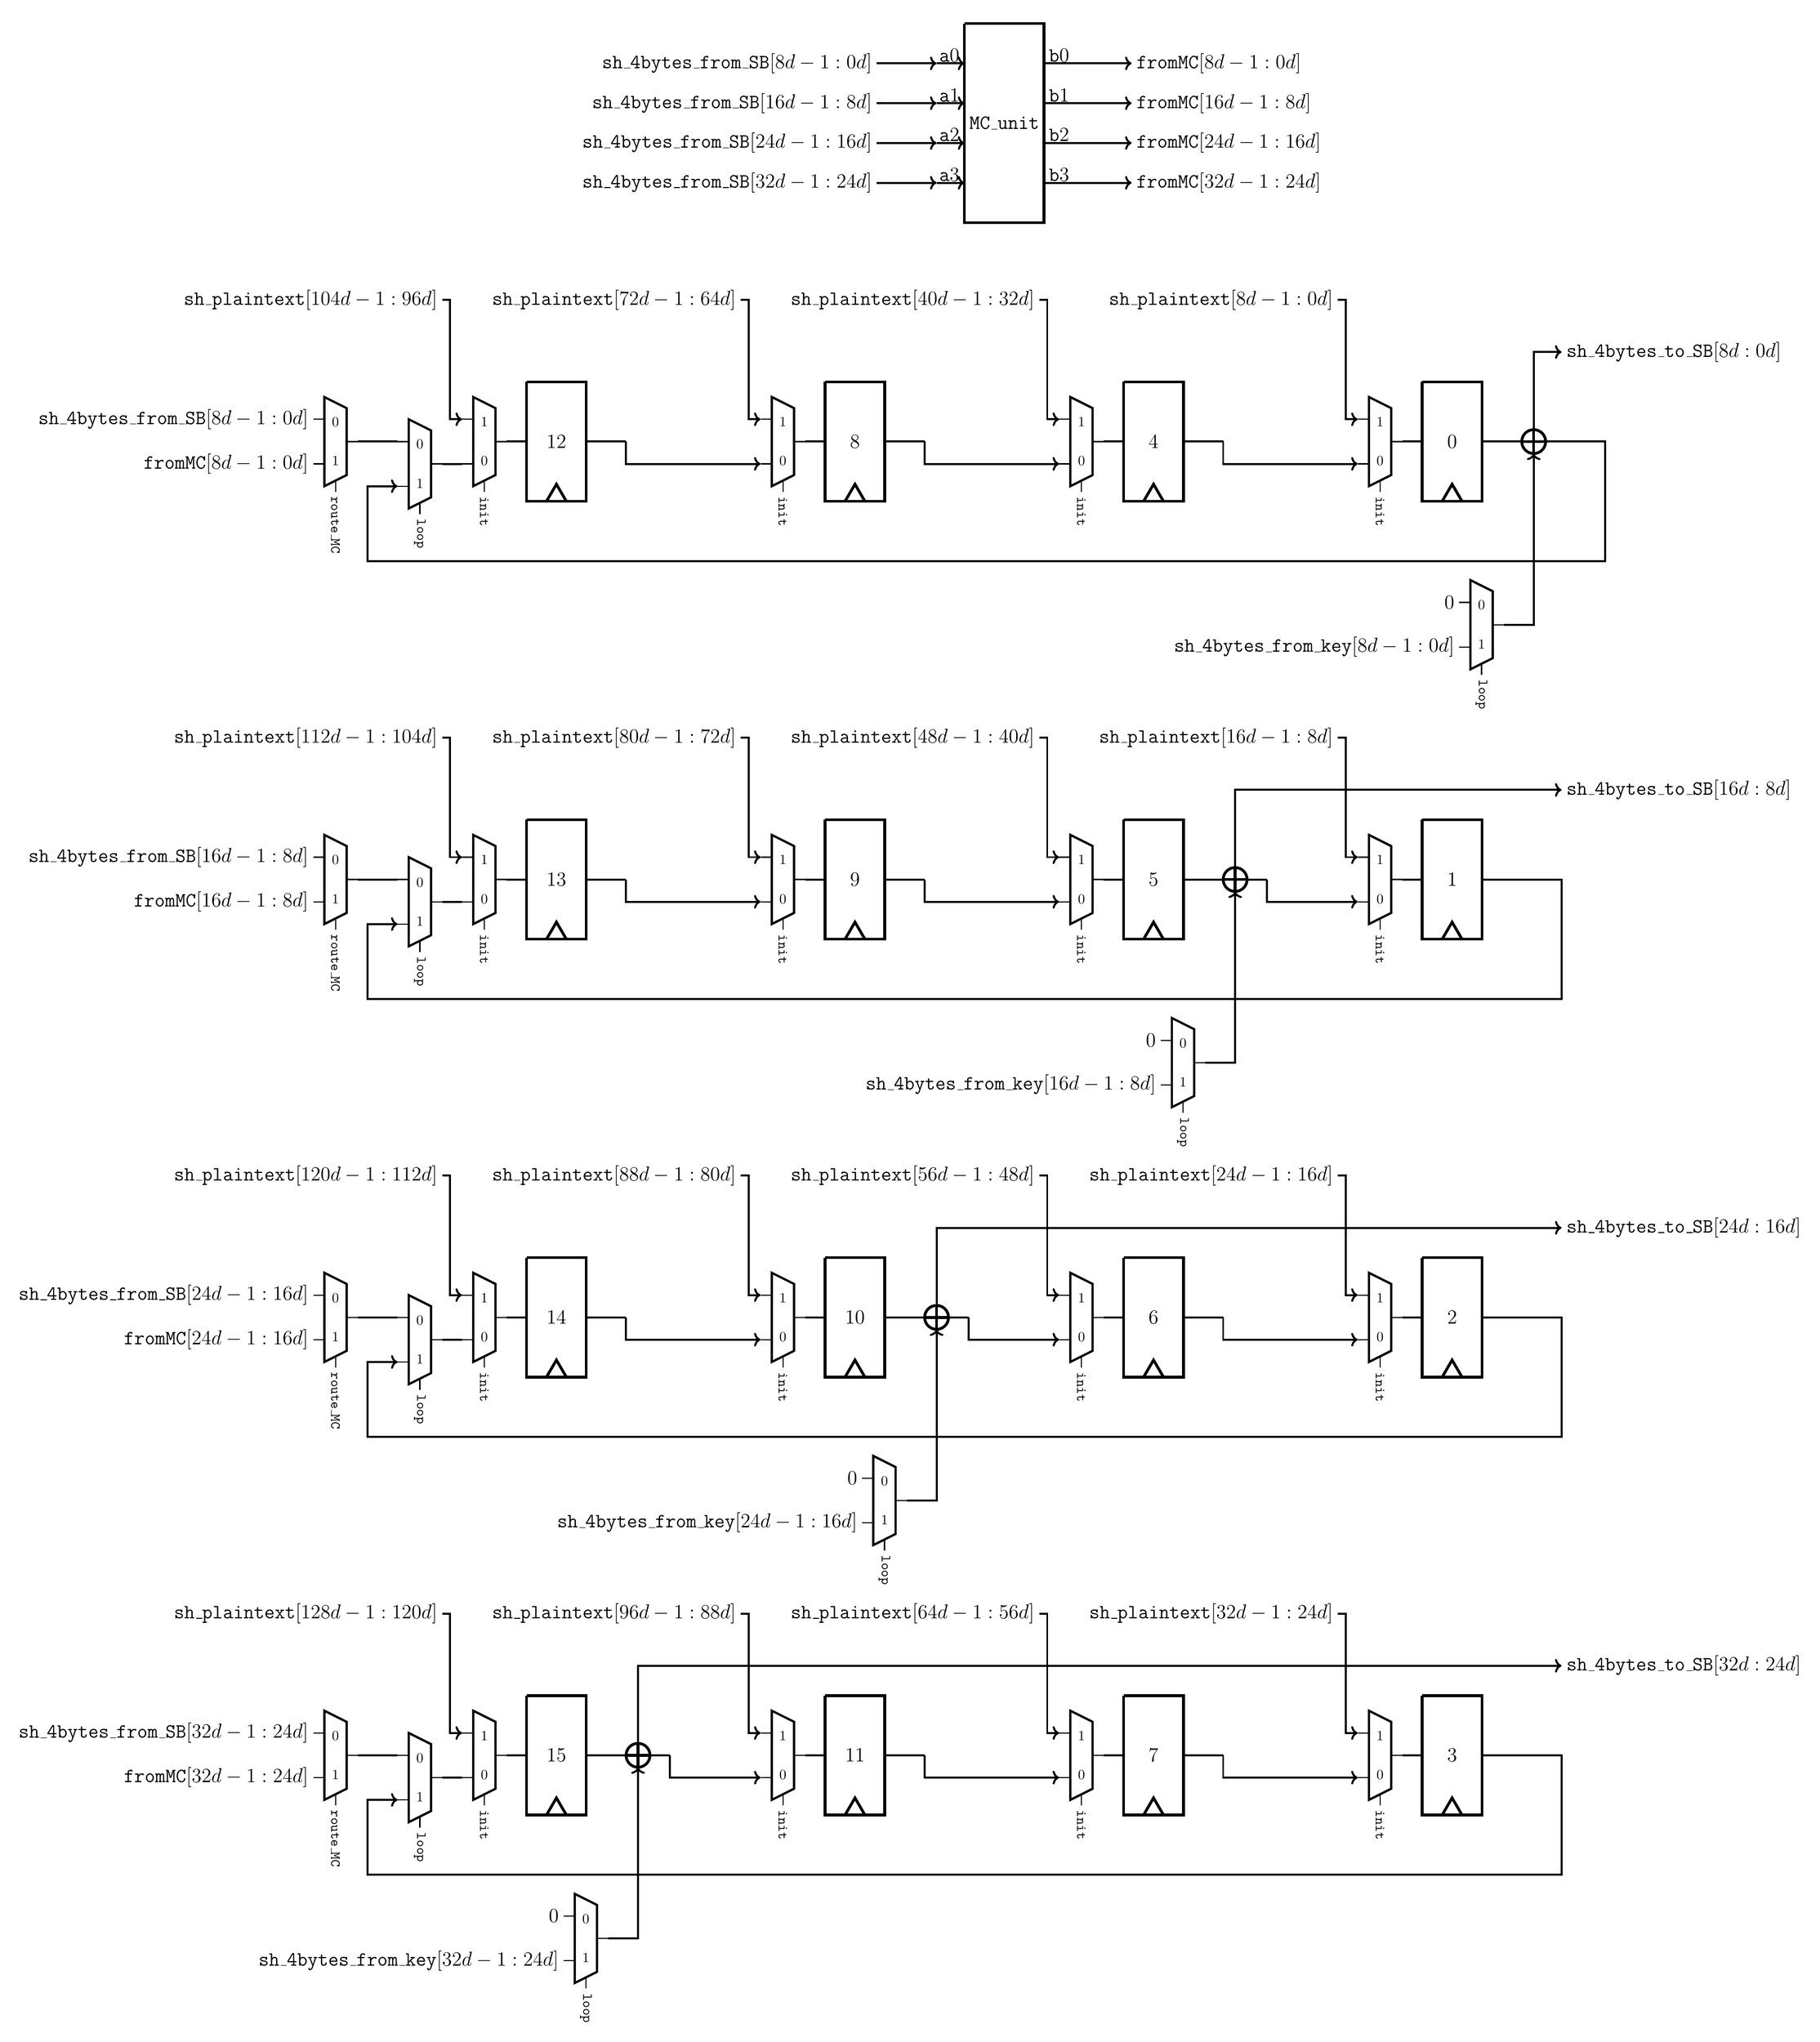
\begin{tikzpicture}
            % define a mux
\tikzset{mux2/.style={muxdemux,muxdemux def={Lh=4, NL=2, Rh=3,NB=1,w=1}}}


%% CONFIG
% Size of DFF instance
\def\widthDFF{1.5}
\def\heightDFF{3}
% Spacing between DFF instance
\def\spacexDFF{7.5}
\def\spaceyDFF{11}
% Spacing after DFF and XOr instance
\def\spaceXOR{0}

% Line width of DFF
\def\lwModule{0.7mm}
\def\lwWire{0.5mm}
\def\scaleCTIKZ{0.4}


\def\spacexFeedBack{0.75}
\def\spacexFeedBackR{2}
\def\spaceyXorOut{0.75*\heightDFF}
\def\spacexXorOut{2}
\def\spaceyFeedBack{3}

\def\spacexIn{0.5}

\def\fontS{\Large}
\def\fontCtrl{}

%\debugtrue;

%% Macro for the ctrl signals of the mux2
% 1: mux_id
% 2: control sig
% 3: top value
% 4: bottom value
\newcommand{\muxCtrl}[4]{
    \node[anchor=west,rotate=270] at (#1.bpin 1) {\fontCtrl #2};
    \node at (#1.center up) {\fontCtrl #3};
    \node at (#1.center down) {\fontCtrl #4};
}

% W internal port macro with annotation
% #1 style
% #2 id
% #3 loc
% #4 text
\def\yshw{2mm}
\def\xshw{2mm}
\newcommand{\portW}[4][]{
    \coordinate (#2) at (#3);
    \node [#1,anchor=east,yshift=\yshw] at (#3) {#4};
}
% E internal port macro with annotation
% #1 style
% #2 id
% #3 loc
% #4 text
\newcommand{\portE}[4][]{
    \coordinate (#2) at (#3);
    \node [#1,anchor=west,yshift=\yshw] at (#3) {#4};
}

% Macro for a bloc with Register with mux input
% #1: style
% #2: id
% #3: loc (center DFF)
\newcommand{\DFFMUX}[3][]{
    % draw DFF
    \DFF[line width=\lwModule]{dffinst}{#3}{\widthDFF}{\heightDFF}
    % draw mux
    \node[line width=\scaleCTIKZ*\lwModule,mux2,anchor=rpin 1, xshift=-0.5cm] (#2/mux) at (dffinst/D) {}; 
    % Connector
    \draw[line width=\lwWire] (#2/mux.rpin 1) -- (dffinst/D);
    % draw small port at Q
    \coordinate (#2/out) at ($(dffinst/Q)+(1,0)$);
    \draw [line width=\lwWire] (dffinst/Q) -- (#2/out);
    % Generate remaining instance coordinate
    \coordinate (#2/text) at (dffinst/center);
    \coordinate (#2/in1) at (#2/mux.lpin 1);
    \coordinate (#2/in2) at (#2/mux.lpin 2);
    \coordinate (#2/ctrl) at (#2/mux.bpin 1);
    % Debug node
    \debugN[out]{(#2/out)}
    \debugN[in1]{(#2/in1)}
    \debugN[in2]{(#2/in2)}
    \debugN[text]{(#2/text)}
    \debugN[ctrl]{(#2/ctrl)}
}

% Macro for a bloc with muxex input key, xor and output port
% #1: style
% #2: id
% #3: loc (west of xor)
\newcommand{\KEYXOR}[3][]{
    \def\Radius{0.3}
    % Draw small port at the input of xor
    \coordinate (#2/inxor) at #3;
    \XOR[line width=\lwModule]{xor}{($(#2/inxor)+(\Radius,0)$)}{\Radius}
    \draw [line width=\lwWire] (#2/inxor) -- (xor/west);
    % Draw the XOR node
    \node[line width=\scaleCTIKZ*\lwModule,mux2,anchor=rpin 1] (#2/mux) at ($(xor/south)+(-0.5*\widthDFF,-1.3-\spaceyFeedBack)$) {};
    \draw [->] [line width=\lwWire] (#2/mux.rpin 1) -| (xor/south);
    % Draw small port at output1
    \coordinate (#2/out1) at (xor/north);
    % Draw small port at output2
    \coordinate (#2/out2) at ($(xor/east) + (0.5,0)$);
    \draw [line width=\lwWire] (xor/east) -- (#2/out2);
    % Generate remaining coordinate
    \coordinate (#2/in1) at (#2/mux.lpin 1);
    \coordinate (#2/in2) at (#2/mux.lpin 2);
    \coordinate (#2/ctrl) at (#2/mux.bpin 1);
    % Debug node
    \debugN[in1]{(#2/in1)}
    \debugN[in2]{(#2/in2)}
    \debugN[out1]{(#2/out1)}
    \debugN[out2]{(#2/out2)}
    \debugN[inxor]{(#2/inxor)}
    \debugN[ctrl]{(#2/ctrl)}
}

%% Macro for a bloc with two input muxes (choosing between from SB and from MC) 
% 1: style
% 2: id 
% 3: loc (out of last mux)
\newcommand{\MUXIN}[3][]{
    % Draw last mux
    \node[line width=\scaleCTIKZ*\lwModule,mux2,anchor=rpin 1] (#2/muxFB) at #3 {};
    \node[line width=\scaleCTIKZ*\lwModule,mux2,anchor=rpin 1,xshift=-1cm] (#2/muxIn) at (#2/muxFB.lpin 1) {};
    \draw [line width=\lwWire] (#2/muxIn.rpin 1) -- (#2/muxFB.lpin 1);
    % Generate coordinate
    \coordinate (#2/out) at #3;
    \coordinate (#2/inFB) at (#2/muxFB.lpin 2);
    \coordinate (#2/inSB) at (#2/muxIn.lpin 1);
    \coordinate (#2/inMC) at (#2/muxIn.lpin 2);
    \coordinate (#2/ctrlFB) at (#2/muxFB.bpin 1);
    \coordinate (#2/ctrlIn) at (#2/muxIn.bpin 1);
    % debug node
    \debugN[out]{(#2/out)}
    \debugN[inFB]{(#2/inFB)}
    \debugN[inSB]{(#2/inSB)}
    \debugN[inMC]{(#2/inMC)}
    \debugN[ctrlFB]{(#2/ctrlFB)}
    \debugN[ctrlIn]{(#2/ctrlIn)}
}

%% Macro for the MC bloc 
% 1: style
% 2: id 
% 3: loc
\newcommand{\MCBloc}[3][]{
    \def\scaleIO{0.7}
    % Draw the MC
    \rectangle[line width=\lwModule]{rec}{#3}{2}{5}{4}{4}{0}{0};
    \node at (rec/center) {\fontS $\dpStateModMC$};
    % Ports declaration
    \foreach \xi in {1,...,4}{
        \pgfmathsetmacro\idxLabel{int(\xi-1)}
        % Input 
        \portW{}{rec/W\xi}{\fontS $\dpStateByteToMC\idxLabel$}
        % Output
        \portE{}{rec/E\xi}{\fontS $\dpStateByteFromMC\idxLabel$}
        % Generate node
        \coordinate (#2/a\xi) at ($(rec/W\xi)+(-\scaleIO,0)$);
        \draw [->, line width=\lwWire] (#2/a\xi) -- (rec/W\xi);
        \coordinate (#2/b\xi) at ($(rec/E\xi)+(\scaleIO,0)$);
        \draw [line width=\lwWire] (rec/E\xi) -- (#2/b\xi);
        % debug node
        \debugN[a\xi]{(#2/a\xi)}
        \debugN[b\xi]{(#2/b\xi)}
    }
}

%%%%% MAIN DRAWING %%%%%%%%%%%%%
\coordinate (D00) at (0,0);

% Draw all the DFFMUX instances
\foreach \xi in {0,...,3} {
    \foreach \yi in {0,...,3} {
        \pgfmathsetmacro\xshDFF{\spacexDFF*\xi}
        \pgfmathsetmacro\yshDFF{\spaceyDFF*\yi}
        \pgfmathsetmacro\DFFindex{int(12-4*\xi+\yi)}
        \DFFMUX{D\DFFindex}{($(D00)+(\xshDFF,-\yshDFF)$)}
        % Compute byte index
        \node at (D\DFFindex/text) {\Large $\DFFindex$};
        % Add the text to the DFF input
        \pgfmathsetmacro\mBound{int(8*\DFFindex)}
        \pgfmathsetmacro\MBound{int(8*(1+\DFFindex))}
        % Add the control of the mux
        \muxCtrl{D\DFFindex/mux}{$\dpStateCtrlRouteIn$}{1}{0}
        % IO plaintext
        \node [anchor=east] (IL) at 
        ($(D\DFFindex/in1)+(-0.5,1.0*\heightDFF)$){\fontS $\AESdpStatePlaintext[\MBound d-1 : \mBound d]$};
        \draw [->,line width=\lwWire] (IL.east) -- ++(0.2,0)  |- (D\DFFindex/in1);
    }
}

%% Compute reference point where to have the x-coordinate of the
% singal to sbox
\coordinate (offsetToSB) at (1,\spaceyXorOut);

% Draw KEYXOR value unit
\foreach \xi in {0,5,10,15}{
    \KEYXOR{KX\xi}{($(D\xi/out)+(\spaceXOR,0)$)}
    % IO ports for KEYXOR
    \pgfmathsetmacro\idxV{int(\xi/5)}
    \pgfmathsetmacro\mB{int(8*\idxV)}
    \pgfmathsetmacro\MB{int(8*(\idxV+1))}
    \node [anchor=east] (Label) at (KX\xi/in2) {\fontS $\AESdpStateFromKey [\MB d-1 : \mB d]$};
    \node [anchor=east] at (KX\xi/in1) {\fontS $0$};  
    %%% Control signal of the mux
    %\node [anchor=west,rotate=270] at (KX\xi/ctrl) {\fontCtrl $\dpStateCtrlRouteLoop$};
    \muxCtrl{KX\xi/mux}{$\dpStateCtrlRouteLoop$}{0}{1}
    %%% IO port out for KEYXOR
    \pgfmathsetmacro\IdxColRight{int(\xi/5)}
    \node [anchor=west] (Label_out) at ($(D\IdxColRight/out)+(offsetToSB)$) {\fontS $\AESdpStateToSB [\MB d : \mB d]$}; 
    \draw [->, line width=\lwWire] (KX\xi/out1) |- (Label_out.west);
}

% Draw the MUXIN structure
\foreach \xi in {12,...,15}{
    \MUXIN{MI\xi}{($(D\xi/in2)+(-\spacexIn,0)$)}
    \draw [line width=\lwWire] (MI\xi/out) -- (D\xi/in2);
    % Add the ctrl signal of the muxes
    \muxCtrl{MI\xi/muxFB}{$\dpStateCtrlRouteLoop$}{0}{1}
    \muxCtrl{MI\xi/muxIn}{$\dpStateCtrlRouteMC$}{0}{1}
}

% Draw the path between registers
\draw [->, line width=\lwWire] (D12/out) |- (D8/in2);
\draw [->, line width=\lwWire] (D8/out) |- (D4/in2);
\draw [->, line width=\lwWire] (D4/out) |- (D0/in2);
\draw [->, line width=\lwWire] (KX0/out2) -| ++(1,-\spaceyFeedBack) -| ($(MI12/inFB)+(-\spacexFeedBack,0)$) -- (MI12/inFB);

\draw [->, line width=\lwWire] (D13/out) |- (D9/in2);
\draw [->, line width=\lwWire] (D9/out) |- (D5/in2);
\draw [->, line width=\lwWire] (KX5/out2) |- (D1/in2);
\draw [->, line width=\lwWire] (D1/out) -| ++(1,-\spaceyFeedBack) -| ($(MI13/inFB)+(-\spacexFeedBack,0)$) -- (MI13/inFB);

\draw [->, line width=\lwWire] (D14/out) |- (D10/in2);
\draw [->, line width=\lwWire] (KX10/out2) |- (D6/in2);
\draw [->, line width=\lwWire] (D6/out) |- (D2/in2);
\draw [->, line width=\lwWire] (D2/out) -| ++(1,-\spaceyFeedBack) -| ($(MI14/inFB)+(-\spacexFeedBack,0)$) -- (MI14/inFB);

\draw [->, line width=\lwWire] (KX15/out2) |- (D11/in2);
\draw [->, line width=\lwWire] (D11/out) |- (D7/in2);
\draw [->, line width=\lwWire] (D7/out) |- (D3/in2);
\draw [->, line width=\lwWire] (D3/out) -| ++(1,-\spaceyFeedBack) -| ($(MI15/inFB)+(-\spacexFeedBack,0)$) -- (MI15/inFB);

% Draw the MC logic bloc and the input of the last column
\MCBloc{MC}{($(D8/text)!0.5!(D4/text) + (0,8)$)}
\foreach \xi in {0,...,3} {
    %% MC value
    \pgfmathsetmacro\mB{int(8*\xi)}
    \pgfmathsetmacro\MB{int(8*(1+\xi))}
    \pgfmathsetmacro\MCidx{int(\xi+1)}
    \node [anchor=east,xshift=-1.5cm] (toMC) at (MC/a\MCidx) {\fontS $\AESdpStateFromSB[\MB d-1:\mB d]$};
    \draw [->,line width=\lwWire] (toMC.east) -- (MC/a\MCidx);
    \node [anchor=west,xshift=1.5cm] (fromMC) at (MC/b\MCidx) {\fontS $\texttt{fromMC}[\MB d-1:\mB d]$};
    \draw [->,line width=\lwWire] (MC/b\MCidx) -- (fromMC.west);
    %% to last column value
    \pgfmathsetmacro\SmB{int(8*(12-\xi))}
    \pgfmathsetmacro\SMB{int(8*(13-\xi))}
    \pgfmathsetmacro\MUXidx{int(12+\xi)}
    \node [anchor=east] (fSBCmux) at (MI\MUXidx/inSB) {\fontS $\AESdpStateFromSB[\MB d-1: \mB d]$};
    \node [anchor=east] (fMCmux) at (MI\MUXidx/inMC) {\fontS $\texttt{fromMC}[\MB d-1:\mB d]$};
}


%




        \end{tikzpicture}
    }
    \caption{Global architecture of the \modAESdpState module. The value held by the DFF at index $i$ is depicted by the signal $\dpStateDFF{i}$ in the HDL.}
    \label{fig:aes_dpState}
\end{figure}

Figure~\ref{fig:aes_dpState} shows the detailed architecture of the
module $\modAESdpState$. It is organized as a shift register where each
register unit holds a masked state byte (the numbers on the figure
indicate the byte index in the unmasked state).
The module operates on 32-bit parts of the state and is also implementing the
logic that computes the $\AK$, $\SR$ and $\MC$ layers, both for the forward and inverse operation.
In particular, these are implemented in purely combinational logic.   

\paragraph{Encryption} When performing an encryption, addition gadgets (i.e., XORs) are used to
perform the key addition with key bytes coming from the round key (denoted
$\AESdpStateFromKey$). The module $\dpStateModMC$ computes the result of the
$\MC$ operation for a masked column (i.e., 4~masked bytes). The $\SR$ layer is
free, being implemented as a specific routing at the input of the $\SB$ layer.
In particular, the ordering of the bytes routed to the S-boxes (denoted
$\AESdpStateToSB$) is selected such that the rotations over the rows are
applied. Dedicated MUXes (controlled by $\dpStateCtrlRouteMC$) are used in
order to bypass the $\MC$ logic block when executing the last round.  Other
MUXes (controlled by $\dpStateCtrlRouteLoop$) are used during the last key
addition in order to bypass the $\SR$, $\SB$ and $\MC$ layers.  When a new
execution starts, the masked plaintext bytes are loaded in the register through
the MUXes controlled by $\dpStateCtrlRouteIn$.  Then, the $\AK$ and $\SR$
layers are executed by propagating the data across the pipeline to the S-boxes
(by selecting the data $\dpStateToSBForward$ with the MUX driving the signal
$\AESdpStateToSB$).  The $\MC$ operation is performed when the result of the
$\SB$ layer is coming back to the core by asserting the signal
$\dpStateCtrlRouteMC$. 

\paragraph{Decryption} When performing a decryption, addition gadget are used to add the key bytes
coming from the round key (denoted
$\AESdpStateFromKeyInverse$). These are located in order to add the key
material with the first column of the state (i.e., bytes indexes in [0,1,2,3]).
The addition gadget located at the byte index 0 is shared between the
encryption and decryption process. The additions outcomes are forwarded to the
module $\dpStateModMCInv$ that implements the inverse $\MC$ operation for a
masked column. A dedicated mux (controlled by $\dpStateCtrlBypassMCInverse$)
allows bypassing the latter, as required when computing the inversion of the
last round. The data are then forward to the S-boxes (by selecting the data
$\dpStateToSBReverse$) in order to compute the inverse $\SB$ layer.  The
inverse $\SR$ layer is implemented by dedicated MUXes that allows to insert the
bytes coming back from the S-boxes to the proper location (i.e., byte indexes in
[12,1,6,11]). Similarly to the key addition, the MUX inserting data at the byte
index 12 is shared between the encryption and the decryption.  

\subsection{Architecture of the $\modAESdpKey$ module}
\label{section:module_dpkey}
\begin{figure}
    \centering
    \resizebox{\textwidth}{!}{
        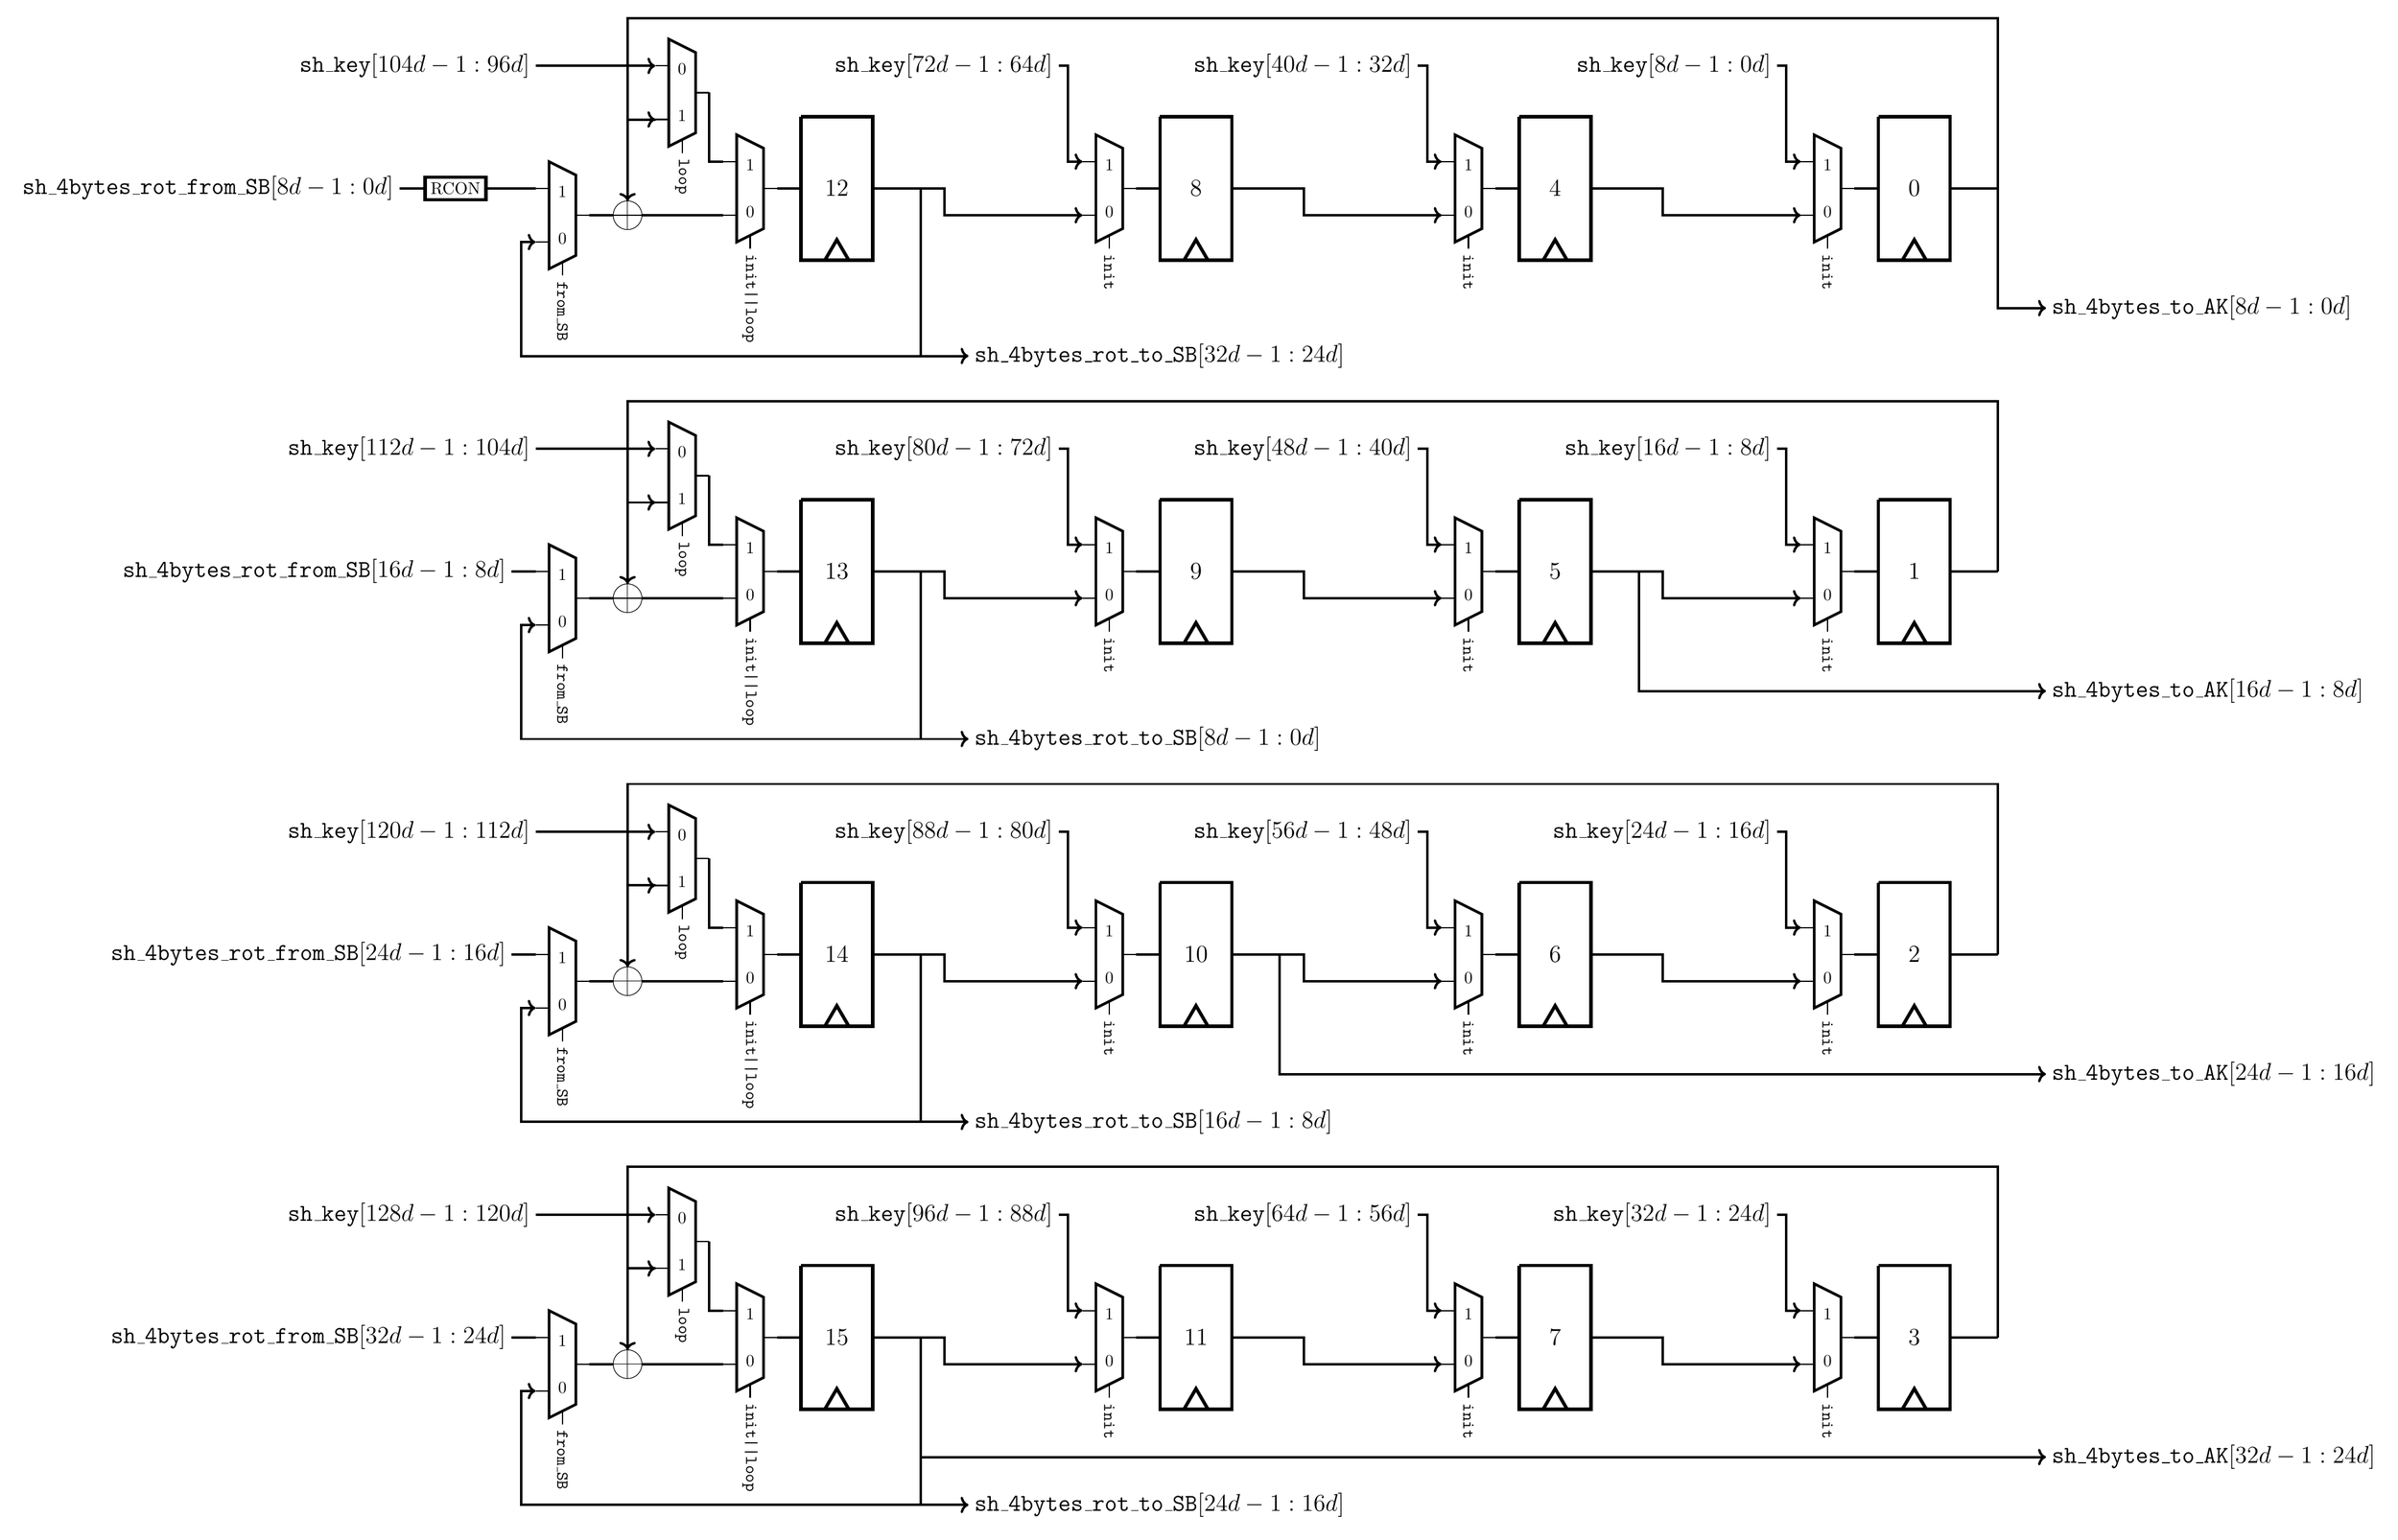
\begin{tikzpicture}
            % define a mux
\tikzset{mux2/.style={muxdemux,muxdemux def={Lh=4, NL=2, Rh=3,NB=1,w=1}}}

%% CONFIG
% Size of DFF instance
\def\widthDFF{1.5}
\def\heightDFF{3}
% Spacing between DFF instance
\def\spacexDFF{7.5}
\def\spaceyDFF{8}
% Y space for last column loop
\def\spaceyLoop{3.5}
% X space for last column input
\def\spacexInLastCol{1}
% Y space for for mux last column
\def\spaceyMuxInLastCol{0.5}

\def\fontS{\Large}
\def\fontCtrl{}

% Line width of DFF
\def\lwModule{0.7mm}
\def\lwWire{0.5mm}
\def\scaleCTIKZ{0.4}


%\debugtrue;

%% Macro for the ctrl signals of the mux2
% 1: mux_id
% 2: control sig
% 3: top value
% 4: bottom value
\newcommand{\muxCtrl}[4]{
    \node[anchor=west,rotate=270] at (#1.bpin 1) {\fontCtrl #2};
    \node at (#1.center up) {\fontCtrl #3};
    \node at (#1.center down) {\fontCtrl #4};
}


% Macro for a bloc with Register with mux input
% #1: style
% #2: id
% #3: loc (center DFF)
\newcommand{\DFFMUX}[3][]{
    % draw DFF
    \DFF[line width=\lwModule]{dffinst}{#3}{\widthDFF}{\heightDFF}
    % draw mux
    \node[line width=\scaleCTIKZ*\lwModule,mux2,anchor=rpin 1, xshift=-0.5cm] (#2/mux) at (dffinst/D) {}; 
    % Connector
    \draw[line width=\lwWire] (#2/mux.rpin 1) -- (dffinst/D);
    % draw small port at Q
    \coordinate (#2/out) at ($(dffinst/Q)+(1,0)$);
    \draw [line width=\lwWire] (dffinst/Q) -- (#2/out);
    % Generate remaining instance coordinate
    \coordinate (#2/text) at (dffinst/center);
    \coordinate (#2/in1) at (#2/mux.lpin 1);
    \coordinate (#2/in2) at (#2/mux.lpin 2);
    \coordinate (#2/north) at (dffinst/north);
    \coordinate (#2/ctrl) at (#2/mux.bpin 1);
    % Debug node
    \debugN[out]{(#2/out)}
    \debugN[in1]{(#2/in1)}
    \debugN[in2]{(#2/in2)}
    \debugN[text]{(#2/text)}
    \debugN[ctrl]{(#2/ctrl)}
}


%%%%% MAIN DRAWING %%%%%%%%%%%%%
\coordinate (D00) at (0,0);

% Draw all the DFFMUX instances
\foreach \xi in {0,...,3} {
    \foreach \yi in {0,...,3} {
        \pgfmathsetmacro\xshDFF{\spacexDFF*\xi}
        \pgfmathsetmacro\yshDFF{\spaceyDFF*\yi}
        \pgfmathsetmacro\DFFindex{int(12-4*\xi+\yi)}
        \DFFMUX{D\DFFindex}{($(D00)+(\xshDFF,-\yshDFF)$)}
        % Compute byte index
        \node at (D\DFFindex/text) {\Large $\DFFindex$};
        % Add the text to the DFF input
        \pgfmathsetmacro\mBound{int(8*\DFFindex)}
        \pgfmathsetmacro\MBound{int(8*(1+\DFFindex))}
    }
}

%%% Generate the input construction at the last column 
% Also generate the feedback loop and the byte to SBox
\foreach \xi in {12,...,15}{
    % Draw the input mux
    \path let \p1=(D\xi/in1), \p2=(D\xi/north) in coordinate (locm) at ($(\x1,\y2)+(-0.3,\spaceyMuxInLastCol)$);
    \node[mux2,line width=\scaleCTIKZ*\lwModule,anchor=rpin 1] (MI\xi) at (locm) {};
    \draw [line width=\lwWire] (MI\xi.rpin 1) |- (D\xi/in1);
    % Create control signal for MUXin
    \muxCtrl{D\xi/mux}{$\dpKeyCtrlRouteScan$}{1}{0}
    \muxCtrl{MI\xi}{$\dpKeyCtrlRouteLoop$}{0}{1}
    % XOR
    \XOR{xor\xi}{($(D\xi/in2)+(-2,0)$)}{0.3}
    \draw [line width=\lwWire] (xor\xi/east) -- (D\xi/in2);
    % Mux at the input of the XOR
    \node[mux2,line width=\scaleCTIKZ*\lwModule,anchor=rpin 1,xshift=-0.5cm] (MX\xi) at (xor\xi/west) {};
    \draw [line width=\lwWire] (MX\xi.rpin 1) -- (xor\xi/west);
    % Draw the ctrl of the mux
    \muxCtrl{MX\xi}{$\dpKeyCtrlRouteFromSB$}{1}{0}
    % Draw the feedback from the register
    \draw [->, line width=\lwWire] (D\xi/out) -- ++(0,-\spaceyLoop) -| ($(MX\xi.lpin 2)+(-0.3,0)$) -- (MX\xi.lpin 2);
    %% Generate feedback port 
    \draw [->,line width=\lwWire] (xor\xi/north) |- (MI\xi.lpin 2);
    \draw [->,line width=\lwWire] (MI\xi.lpin 2) -| (xor\xi/north);
    % Generate the coordinate of the ports
    \path let \p1=(MI\xi.lpin 2), \p2=(xor\xi/north) in coordinate (FB\xi) at (\x2,\y1);
    \debugN[FB\xi]{(FB\xi)}
    %% Generate key input
    \path let \p1=(MX\xi.lpin 1), \p2=(MI\xi.lpin 1) in coordinate (inKey\xi) at (\x1,\y2);
    \debugN[inKey\xi]{(inKey\xi)}
    \draw [->,line width=\lwWire] (inKey\xi) -- (MI\xi.lpin 1);
    %% Generate Sbox input
    \coordinate (fromSB\xi) at (MX\xi.lpin 1); 
    \debugN[fromSB\xi]{(fromSB\xi)}
    %% Generate feedback loop
    \pgfmathsetmacro\rIdx{int(\xi-12)}
    \path let \p1=(inKey\xi), \p2=(D\rIdx/out) in coordinate (tmp) at (\x2,\y1);
    \coordinate (tmp1) at ($(tmp)+(0,1)$);
    \draw [line width=\lwWire] (D\rIdx/out) -- (tmp1) -| (FB\xi);
    %% Draw input nodes
    % to Sbox
    \coordinate (toSB\xi) at ($(D\xi/out)+(1,-\spaceyLoop)$);
    \debugN[toSB\xi]{(toSB\xi)}
    % to AK
    \pgfmathsetmacro\idxAK{int(\xi-12)}
    \coordinate (toAK\idxAK) at ($(D\idxAK/out)+(1,-\spaceyLoop+1)$);
    \debugN[toAK\idxAK]{(toAK\idxAK)}
    % Key in 
    \pgfmathsetmacro\mB{int((\xi)*8))}
    \pgfmathsetmacro\MB{int((\xi+1)*8)}
    \node [anchor=east] at (inKey\xi) {\fontS $\AESdpKeyKey[\MB d-1: \mB d]$};

}

%% Draw the port to SB
\node [anchor=west] at (toSB12) {\fontS $\AESdpKeyToSB[32d-1:24d]$};
\node [anchor=west] at (toSB13) {\fontS $\AESdpKeyToSB[8d-1:0d]$};
\node [anchor=west] at (toSB14) {\fontS $\AESdpKeyToSB[16d-1:8d]$};
\node [anchor=west] at (toSB15) {\fontS $\AESdpKeyToSB[24d-1:16d]$};
\draw [->,line width=\lwWire] (D12/out) |- (toSB12);
\draw [->,line width=\lwWire] (D13/out) |- (toSB13);
\draw [->,line width=\lwWire] (D14/out) |- (toSB14);
\draw [->,line width=\lwWire] (D15/out) |- (toSB15);

%%% Generate the inport port for columns other than last ones
%%% Generate also input connexions for the DFF units
\foreach \xi in {0,...,3}{
    \foreach \yi in {0,...,2}{
        % Fetch y coordinate of the input mux of last column
        \pgfmathsetmacro\refIdx{int(12+\xi)}
        \pgfmathsetmacro\DIdx{int(\xi+4*\yi)}
        \coordinate (refP) at (MI\refIdx.lpin 1);
        \path let \p1=(refP), \p2=(D\DIdx/in1) in coordinate (inKey\DIdx) at ($(\x2,\y1) + (-0.5,0)$);  
        \debugN[inKey\DIdx]{(inKey\DIdx)}
        \draw [->,line width=\lwWire] (inKey\DIdx) -- ++(0.2,0) |- (D\DIdx/in1);
        %% Input connexion
        \pgfmathsetmacro\DIdxp{int(\xi+4*(\yi+1))}
        \draw [->,line width=\lwWire] (D\DIdxp/out) -- ++(0.5,0) |- (D\DIdx/in2);
        %% Draw input port
        \pgfmathsetmacro\mB{int(8*\DIdx)}
        \pgfmathsetmacro\MB{int(8*(\DIdx+1))}
        \node [anchor=east] at (inKey\DIdx) {\fontS $\AESdpKeyKey[\MB d-1:\mB d]$};
        %% Draw mux ctrl
        \muxCtrl{D\DIdx/mux}{$\dpKeyCtrlRouteInit$}{1}{0}
    }
}

%%% Generate input for the last column
\node [line width=\lwModule,rectangle,draw,anchor=east] (RCON) at ($(fromSB12)+(-\spacexInLastCol,0)$) {RCON};
\node [anchor=east,xshift=-0.5cm] (fSB12) at (RCON.west) {\fontS $\AESdpKeyFromSB[8d-1:0d]$};
\draw [line width=\lwWire] (RCON.east) -- (fromSB12) (fSB12.east) -- (RCON.west);

\node [anchor=east,xshift=-0.5cm] (fSB13) at (fromSB13) {\fontS $\AESdpKeyFromSB[16d-1:8d]$};
\node [anchor=east,xshift=-0.5cm] (fSB14) at (fromSB14) {\fontS $\AESdpKeyFromSB[24d-1:16d]$};
\node [anchor=east,xshift=-0.5cm] (fSB15) at (fromSB15) {\fontS $\AESdpKeyFromSB[32d-1:24d]$};

\foreach \xi in {13,14,15}{
    \draw [line width=\lwWire] (fSB\xi) -- (fromSB\xi);
}

%%% Generate out for bytes_to_AK
\foreach \xi in {0,...,3}{
    \pgfmathsetmacro\idxStart{int(5*\xi)}
    \pgfmathsetmacro\mB{int(8*\xi)}
    \pgfmathsetmacro\MB{int(8*(\xi+1))}
    \node [anchor=west] at (toAK\xi) {\fontS $\AESdpKeyToAK[\MB d-1:\mB d]$};
    \draw [->, line width=\lwWire] (D\idxStart/out) |- (toAK\xi);
}


        \end{tikzpicture}
    }
    \caption{Global architecture of the module $\modAESdpKey$. The value held by the DFF at index $i$ is depicted by the signal $\dpKeyDFF{i}$ in the HDL.}
    \label{fig:aes_dpKey}
\end{figure}

The module $\modAESdpKey$ is shown in Figure~\ref{fig:aes_dpKey}. It is
organized as a shift register where each register unit holds a masked byte of
the key. The module is split in 4~independent parts, each taking care of the
key scheduling operation on a single row. The sharing of the key is routed from
the input with the control signal $\dpKeyCtrlInit$. Depending on the key size
configured, some part of the bus $\AESdpKeyKey$ may contain 'dont care' values
and some registers are turned off. In particular, the bytes indexes from 16 to
31 are not used in the 128-bit key version (i.e., registers are disabled) and
the bytes indexes from 24 to 31 are initially considered as holding 'dont care'
value in the 192-bit key version.

Two relevant bytes ordering are depicted on the Figure and both refers to the
byte index in the unmasked key. First, the numbers on the top depict the
register location and correspond to the byte ordering at the beginning of a
round when the key addition occurs (the byte ordering is relative to the round
execution flow). Second, the bottom number (between parentheses) depict the
byte ordering when a fresh execution starts, at the last cycle of a round or
when the $\SB$ layer results of the key scheduling are fetched back from the
S-boxes, as detailed next. In practice, the second ordering corresponds to the
first one with a rotation of 1 column to the left when considering the first 4
columns only. The structure composed of the registers driven by MUXes that are
controlled with the signal $\dpKeyCtrlRstBuffer$ as well ass the XORs they are
driving are not used during encryptions (i.e., $\dpKeyCtrlRstBuffer$ is constantly set to
'1'). 

\paragraph{AES-128 Encryption} When computing a 128-bit encryption, the key scheduling starts by sending the
last column of the key (i.e., byte indexes 12, 13, 14 and 15, but that are
located in positions 0,1,2 and 3) to the S-boxes.  To do so, the signals
$\dpKeyCtrlReverseDefaut$ and $\dpKeyCtrlColSevenToSB$ are set to '0' in order
to let the data pass through the MUXes up to the output of the core.  The
$\texttt{RotWord}$ operation is performed by using an appropriate routing of
the signal $\AESdpKeyToSB$ that sends the key bytes to the S-boxes.  Once
computed, the result of the $\SB$ layer is routed back to the core through the
MUX controlled by the signal $\dpKeyCtrlRouteFromSB$, by setting to '0' the signal $\dpKeyCtrlDisableRot$.  At the same time, the
round constant is applied and the first column (i.e., byte indexes 0,1,2 and 3)
of the new round key is computed by adding the first column of the key (thus located in positions 4,5,6 and 7) to the column coming back from
the S-boxes. The remaining three columns (i.e., byte indexes [4,5,6,7],
[8,9,10,11] and [12,13,14,15]) are then updated sequentially by XORing each
byte with the value of the last byte updated in the same row. 
The signal $\dpKeyCtrlLoop$ is used to make the key shares loop across the key
pipeline.  This is required to keep the key material after the $\AK$ operations
while the $\SB$ results of the key scheduling is still under computation. 

\paragraph{AES256 Encryption}The architecture required for the 256-bit encryption is built upon the 128-bit
one, and presents some specificities detailed next. The signal
$\dpKeyCtrlColSevenToSB$ is asserted at the very first cycle of an execution in
order to send the seventh column of the key (i.e., bytes indexes 28,29,30 and
31) instead of the fourth one, accordingly with the 256-bit version
specifications. It is de-asserted for the remaining of the execution. When new
round key material are computed, the registers at positions 16 to 31 are
enabled in order to store these. In the same time, the data hold in these
registers are propagated through the pipeline by asserting the signal
$\dpKeyCtrlFBFromHigh$. The MUX controlled by the signal $\dpKeyCtrlDisableRot$
allows bypassing the addition of the round constant together with
$\texttt{RotWord}$ operation, as required by one round out of two with the
256-bit version. 

\paragraph{AES-128/256 Decryption} Naively, the inversion of the key scheduling can be implemented by performing
the inverse operation of the key schedule algorithm, in reverse order. That is,
considering that a round key is composed of 4 columns of 32-bit, the three last
columns of an update key can be computed by sequentially XORing the last three
columns of the current key.  For the first column, one must additionnally XOR
the result of the $\SB$ operation applied to the last column of the updated
key, obtained as described above by XORing the two last columns of the current
key (that is, the two columns composed of the key bytes at indexes
[12,13,14,15] and [8,9,10,11]). As a reminder, the 256-bit version does not
require the \texttt{RotWord} operation and the addition of the round constant
at every round, which can be disabled by properly driving the signal
$\dpKeyCtrlDisableRot$. Implementing this exact computational flow would at
least require to route the data through the pipeline in the opposite direction
to what is already implemented for the encryption, leading to significant area
overhead (e.g., at least $128d$ MUXes and logic replication). Instead, the core
stick the data propagation flow of the encryption and implements the inverse
key schedule as detailed next. First, the last column of the updated key is
computed by XORing the last two columns. In parallel, the latter is routed to
the S-boxes by asserting the signal $\dpKeyCtrlReverseDefaut$.  Next, the key
update is similar to what is done during an encryption. That is, the first
column of the updated key is computed by XORing the first column of the current
key (located at the positions 4,5,6 and 7) with the material coming back from
the S-boxes. The following three columns are computed sequentially by XORing the
freshly updated column (located at positions 0,1,2 and 3) with the column of
the current key (located at positions 4,5,6 and 7). Aditionally, the signal
$\dpKeyCtrlRstBuffer$ is asserted for 4 consecutive cycles in order to
accumulate the value coming back from the S-boxes with the sequential freshly
updated key columns.  The latter mechanism is required for functionality
purpose of the algorithm. Similarly to hte encryption process, the freshly
updated key material are propagated through the pipeline, either to the
locations [12,13,14,15] for the 128-bit version, either to the locations
[28,29,30,31] for the 256-bits version. 

\paragraph{AES-192}
The 192-bit version of the algorithm takes advantage of the existing
structure and is implemented without any additional logic apart from specific
control.  

\subsection{Internal operations}

\paragraph{Overview}
For the three version of the algorithm, the round computations (i.e.,
computation occurring inside the module $\modAESdpState$) are performed in
parallel to the key schedule (i.e., computations occurring inside the module
$\modAESdpKey$).

As the structure of the 128-bit and 256-bit versions are reasonably similar,
they benefit from the same performance in terms of latency, whether for
encryption or decryption.  The latter is equal to $1+\Nr\cdot(8)+4$ cycles,
where $\Nr = 10$ and $\Nr= 14$ for the 128-bit and 256-bit versions
respectively. The first cycle (i.e., the '1' in the equation) correspond to the
cycle where the first key material are sent to the S-boxes in order to start the
key update mechanism. Then, the $\Nr$ round are executed sequentially, each of
them requiring 8 cycles to proceed.  Finally, the final key addition is
performed in 4 cycles. 

Due to the fact that there is less structural similarity between the rounds
computations (which consist in applying the same operation on 128-bit states)
and the evolution of the key (which consist in applying the same operation on
192-bit parts), the implementation requiring no additional logic described in
Section~\ref{section:module_dpkey} comes at the cost of a significant latency
overhead. The latter is directly caused by the complexity of computing the key
scheduling part without modifying the existing module. The flow followed by the
round computations taking place inside the module $\modAESdpState$ is not
modified, with the difference that the registers are stalled at the end of a
round computation to allow the next key computation to be completed before
starting the next round.  Its implementation consists of a complex control of
the existing pipeline, making it possible to implement a step that updates 18
successive key columns in 49 cycles during an encryption (resp. 29 during a
decryption) and that is repeated 4 times to achieve a complete update.
Similarly to the other version, the first cycle of an execution is not related
to the round computation, but is rather used in the context of the 192-bit
version to ensure a proper ordering of the key bytes before starting a round
computation. Also, the final key addition is performed in 4 additional cycles. 

\paragraph{Detailed AES-128 Encryption flow}
Let us first introduce notations for the intermediate states in the AES algorithm with
pseudo-code in Figure~\ref{fig:code_round} and Figure~\ref{fig:code_key}.
Each variable denotes a state or subkey byte at a given step of the algorithm.
In particular, the plaintext (resp. key, ciphertext) byte at index $0\leq i<16$
is denoted \pP{i} (resp. $\pK{i}$, $\pCt{i}$), and the value $\pS{i}{r}$ (resp.
$\pRK{i}{r}$) denotes the byte at index $i$ of the state (resp. round key)
starting the $r$-th round.
When no index is given, the full 128-bit state is considered instead.

\begin{figure}
    \begin{lstlisting}[frame=single]
    %%% First key addition
    for $0\leq i <16$ do
        $\pS{i}{0} = \pP{i} \oplus \pK{i}$;
    done
    
    %%% Perform the rounds
    for $0\leq r < 9$ do 
        % Operation for a single round
        $\pSR{}{r} = \SR(\pS{}{r})$;
        $\pSB{}{r} = \SB(\pSR{}{r})$;
        $\pMC{}{r} = \MC(\pSB{}{r})$;
        $\pAK{}{r} = \AK(\pMC{}{r},\pRK{}{r})$;
        $\pS{}{r+1} = \pAK{}{r}$;
    done
    
    %%% Last round
    $\pSR{}{9}=\SR(\pS{}{9})$;
    $\pSB{}{9}=\SB(\pSR{}{9})$;
    $\pAK{}{9}=\AK(\pSB{}{9})$;
    $\pCt{} = \pAK{}{9}$;
    \end{lstlisting}
    \caption{Pseudo-code of the AES encryption.}
    \label{fig:code_round}
\end{figure}


\begin{figure}
    \begin{lstlisting}[frame=single]
    %%% Key evolution for each round key 
    for $0\leq r < 10$ do
        % Fetch value on which operate
        if $r==0$ then
            $t^r = \pK{}$; 
        else 
            $t^r = \pRK{}{r-1}$;
        end

        % Perform the last column rotation
        $[\pR{0}{r},\pR{1}{r},\pR{2}{r},\pR{3}{r}] = [t_{13}^{r},t_{14}^{r},t_{15}^{r},t_{12}^{r}]$; 

        % Perform SubWord on the rotated column
        $[\pRSB{0}{r},\pRSB{1}{r},\pRSB{2}{r},\pRSB{3}{r}] = [\SW{\pR{0}{r}},\SW{\pR{1}{r}},\SW{\pR{2}{r}},\SW{\pR{3}{r}}]$

        % Compute the first column of the next round key
        $\pRK{0}{r} = \pRSB{0}{r} \oplus t_{0}^{r} \oplus \RCON{r}$;
        $\pRK{1}{r} = \pRSB{1}{r} \oplus t_{1}^{r}$;
        $\pRK{2}{r} = \pRSB{2}{r} \oplus t_{2}^{r}$;
        $\pRK{3}{r} = \pRSB{3}{r} \oplus t_{3}^{r}$;

        % Generate the three remaining columns
        for $1\leq i <4$ do
            for $0\leq j <4$ do
                $\pRK{4i+j}{r} = \pRK{4(i-1)+j}{r} \oplus t_{4i+j}^{r}$;
            done
        done
    done
    \end{lstlisting}
    \caption{Pseudo-code for the AES-128 key evolution.}
    \label{fig:code_key}
\end{figure}

\begin{figure}
    \centering
    \begin{tikztimingtable}
\texttt{clk} & L15{HL}\\
\\
\timeCnrRound & D2{DD}{$i-1$} 10{DD}{$i$} 2{DD}{$i+1$} \\
\timeCnrCycle & D{7} 2D{8} 2D{9} 2D{0}2D{1}2D{2}2D{3}2D{4}2D{5}2D{6}2D{7}2D{8}2D{9}2D{0}2D{1} \\
\\
\AESsboxIn $[8d-1:0]$&3D{0} \cDP{$\pRK{13}{i-1}$} \cDP{$\pS{0}{i}$} \cDP{$\pS{4}{i}$}  \cDP{$\pS{8}{i}$} \cDP{$\pS{12}{i}$} 5{DD}{0} \cDP{$\pRK{13}{i}$} \cDP{$\pS{0}{i+1}$} \cDP{$\pS{4}{i+1}$}\\
\AESsboxIn $[16d-1:8d]$&3D{0} \cDP{$\pRK{14}{i-1}$} \cDP{$\pS{5}{i}$} \cDP{$\pS{9}{i}$}  \cDP{$\pS{13}{i}$} \cDP{$\pS{1}{i}$} 5{DD}{0} \cDP{$\pRK{14}{i}$} \cDP{$\pS{5}{i+1}$} \cDP{$\pS{9}{i+1}$}\\
\AESsboxIn $[24d-1:16d]$&3D{0} \cDP{$\pRK{15}{i-1}$} \cDP{$\pS{10}{i}$} \cDP{$\pS{14}{i}$}  \cDP{$\pS{2}{i}$} \cDP{$\pS{6}{i}$} 5{DD}{0} \cDP{$\pRK{15}{i}$} \cDP{$\pS{10}{i+1}$} \cDP{$\pS{14}{i+1}$}\\
\AESsboxIn $[32d-1:24d]$&3D{0} \cDP{$\pRK{12}{i-1}$} \cDP{$\pS{15}{i}$} \cDP{$\pS{3}{i}$}  \cDP{$\pS{7}{i}$} \cDP{$\pS{11}{i}$} 5{DD}{0} \cDP{$\pRK{12}{i}$} \cDP{$\pS{15}{i+1}$} \cDP{$\pS{3}{i+1}$}\\
\\
\AESsboxOut $[8d-1:0]$&D{} \cDP{$\pSB{8}{i-1}$} \cDP{$\pSB{12}{i-1}$} 5{XX} \cDP{\pRSB{0}{i}} \cDP{$\pSB{0}{i}$}\cDP{$\pSB{4}{i}$}\cDP{$\pSB{8}{i}$}\cDP{$\pSB{12}{i}$} 2{XX}\\
\AESsboxOut $[16d-1:8d]$&D{} \cDP{$\pSB{9}{i-1}$} \cDP{$\pSB{13}{i-1}$} 5{XX} \cDP{\pRSB{1}{i}} \cDP{$\pSB{1}{i}$}\cDP{$\pSB{5}{i}$}\cDP{$\pSB{9}{i}$}\cDP{$\pSB{13}{i}$} 2{XX} \\
\AESsboxOut $[24d-1:16d]$&D{} \cDP{$\pSB{10}{i-1}$} \cDP{$\pSB{14}{i-1}$} 5{XX} \cDP{\pRSB{2}{i}} \cDP{$\pSB{2}{i}$}\cDP{$\pSB{6}{i}$}\cDP{$\pSB{10}{i}$}\cDP{$\pSB{14}{i}$} 2{XX} \\
\AESsboxOut $[32d-1:24d]$&D{} \cDP{$\pSB{11}{i-1}$} \cDP{$\pSB{15}{i-1}$} 5{XX} \cDP{\pRSB{3}{i}} \cDP{$\pSB{3}{i}$}\cDP{$\pSB{7}{i}$}\cDP{$\pSB{11}{i}$}\cDP{$\pSB{15}{i}$} 2{XX} \\
\extracode
\makeatletter
\begin{pgfonlayer}{background}
    % Draw cycles
    \begin{scope}[gray,semitransparent,semithick]
        \foreach \x in {1,3,...,27}{
            \draw (\x,1.5) -- (\x,-26.5);
        }
    \end{scope}
    % Draw round
    \foreach \x in {5,25}{
        \draw [thick] (\x,2) -- (\x,-27);
    }
\end{pgfonlayer}
\end{tikztimingtable}

    \caption{Data going into / coming from the S-boxes during an encryption round of AES-128.}
    \label{fig:pipe_sbox}
\end{figure}


\begin{figure}
    \centering
    \begin{tikztimingtable}
\texttt{clk} & L11{HL}\\
\\
\timeCnrRound & D1{DD}{$i-1$} 8{DD}{$i$} 2{DD}{$i+1$} \\
\timeCnrCycle & D{6} 2D{7} 2D{0} 2D{1}2D{2}2D{3}2D{4}2D{5}2D{6}2D{7}2D{0}2D{1} \\
\\
\dpKeyDFF{0} & \timeLinedpKeyI{0}{4}{8}{12} \\ 
\dpKeyDFF{1} & \timeLinedpKeyI{1}{5}{9}{13} \\ 
\dpKeyDFF{2} & \timeLinedpKeyI{2}{6}{10}{14} \\ 
\dpKeyDFF{3} & \timeLinedpKeyI{3}{7}{11}{15} \\ 
\\
\dpKeyDFF{4} & \timeLinedpKeyII{4}{8}{12}{0}  \\
\dpKeyDFF{5} & \timeLinedpKeyII{5}{9}{13}{1}  \\
\dpKeyDFF{6} & \timeLinedpKeyII{6}{10}{14}{2} \\
\dpKeyDFF{7} & \timeLinedpKeyII{7}{11}{15}{3} \\
\\
\dpKeyDFF{8} & \timeLinedpKeyIII{8}{12}{0}{4} \\
\dpKeyDFF{9} & \timeLinedpKeyIII{9}{13}{1}{5} \\
\dpKeyDFF{10} & \timeLinedpKeyIII{10}{14}{2}{6} \\
\dpKeyDFF{11} & \timeLinedpKeyIII{11}{15}{3}{7} \\
\\
\dpKeyDFF{12} & \timeLinedpKeyIIII{12}{0}{4}{8}  \\
\dpKeyDFF{13} & \timeLinedpKeyIIII{13}{1}{5}{9}  \\
\dpKeyDFF{14} & \timeLinedpKeyIIII{14}{2}{6}{10} \\
\dpKeyDFF{15} & \timeLinedpKeyIIII{15}{3}{7}{11} \\
\extracode
\makeatletter
\begin{pgfonlayer}{background}
    % Draw cycles
    \begin{scope}[gray,semitransparent,semithick]
        \foreach \x in {1,3,...,23}{
            \draw (\x,1.5) -- (\x,-46.5);
        }
    \end{scope}
    % Draw round
    \foreach \x in {3,19}{
        \draw [thick] (\x,2) -- (\x,-47);
    }
\end{pgfonlayer}
\end{tikztimingtable}

    \caption{Data going into / coming from the key scheduling datapath during an encryption round of AES-128.}
    \label{fig:pipe_dpkey}
\end{figure}

\begin{figure}
    \centering
    \begin{tikztimingtable}
\texttt{clk} & L15{HL}\\
\\
\timeCnrRound & D2{DD}{$i-1$} 10{DD}{$i$} 2{DD}{$i+1$} \\
\timeCnrCycle & D{7} 2D{8} 2D{9} 2D{0}2D{1}2D{2}2D{3}2D{4}2D{5}2D{6}2D{7}2D{8}2D{9}2D{0}2D{1} \\
\\
\dpStateDFF{0} & \timeLinedpStateZ{0}{4}{8}{12}\\ 
\dpStateDFF{1} & \timeLinedpStateI{1}{5}{9}{13}\\ 
\dpStateDFF{2} & \timeLinedpStateII{2}{6}{10}{14} \\ 
\dpStateDFF{3} & \timeLinedpStateIII{3}{7}{11}{15} \\ 
\\
\dpStateDFF{4} & \timeLinedpStateIV{4}{8}{12}{0} \\
\dpStateDFF{5} & \timeLinedpStateV{5}{9}{13}{1} \\
\dpStateDFF{6} & \timeLinedpStateVI{6}{10}{14}{2} \\
\dpStateDFF{7} & \timeLinedpStateVII{7}{11}{15}{3} \\
\\
\dpStateDFF{8} & \timeLinedpStateVIII{8}{12}{0}{4}\\
\dpStateDFF{9} & \timeLinedpStateIX{9}{13}{1}{5}\\
\dpStateDFF{10} & \timeLinedpStateX{10}{14}{2}{6}\\
\dpStateDFF{11} & \timeLinedpStateXI{11}{15}{3}{7} \\
\\
\dpStateDFF{12} & \timeLinedpStateXII{12}{0}{4}{8} \\
\dpStateDFF{13} & \timeLinedpStateXIII{13}{1}{5}{9} \\
\dpStateDFF{14} & \timeLinedpStateXIV{14}{2}{6}{10} \\
\dpStateDFF{15} & \timeLinedpStateXV{15}{3}{7}{11} \\
\extracode
\makeatletter
\begin{pgfonlayer}{background}
    % Draw cycles
    \begin{scope}[gray,semitransparent,semithick]
        \foreach \x in {1,3,...,27}{
            \draw (\x,1.5) -- (\x,-46.5);
        }
    \end{scope}
    % Draw round
    \foreach \x in {5,25}{
        \draw [thick] (\x,2) -- (\x,-9);
        \draw [thick] (\x,-16) -- (\x,-19);
        \draw [thick] (\x,-26) -- (\x,-29);
        \draw [thick] (\x,-36) -- (\x,-39);
        \draw [thick] (\x,-46) -- (\x,-47);
    }
\end{pgfonlayer}
\end{tikztimingtable}

    \caption{Data going into / coming from the round function datapath during an encryption round of AES-128.}
    \label{fig:pipe_dpstate}
\end{figure}


\begin{figure}
    \centering
    \begin{tikztimingtable}
        \texttt{clk} & L13{HL}\\
        \\
        \timeCnrExecCycles & 5D{0}2D{0}2D{1}2D{2}2D{3}2D{4}2D{5}2D{6}2D{7}2D{8}2D{9}2D{10} \\
        \timeCnrRound & D2{DD}{0} 9{DD}{0} 2{DD}{1} \\
        \timeCnrCycle & D2{DD}{0} 4D{0}2D{1}2D{2}2D{3}2D{4}2D{5}2D{6}2D{7}2D{0}2D{1} \\
        \\ 
        {\color{red} \topModAES} \\
        \portAESInValid & L1{LL}1{HH} 11{LL} \\
        \portAESbusy & L2{LL} 11{HH} \\
        \\
        \AESFetchIn & L1{LL}1{HH} 11{LL}\\
        \AESsboxFeedKey & L2{LL} 2H 7{LL} 2H 2{LL}\\
        \AESsboxValidIn & L2{LL} 5{HH} 3{LL} 3{HH}\\
        \AESsboxValidOut & L3{LL} 3{LL} 5{HH} 2{LL}\\
        \portAESOutValid & L13{LL}\\
        \\
        {\color{red} \modAESdpState}  \\
        \dpStateCtrlEnable & H1{HH}1{HH}1{LL}3{HH}1{LL}6{HH} \\
        \dpStateCtrlRouteIn & H1{HH}1{HH}11{LL} \\
        \dpStateCtrlRouteLoop & L3{LL} 4{HH} 4{LL} 2{HH}\\
        \dpStateCtrlRouteMC & L3{LL}10{HH} \\
        \\
        {\color{red} \modAESdpKey} \\
        \dpKeyCtrlEnable & H1{HH}1{HH}1{HH} 4{HH} 1{HH} 4{HH} 1{HH}\\
        \dpKeyCtrlRouteInit & H1{HH}1{HH}11{LL} \\
        \dpKeyCtrlRouteLoop & L2{LL} 5{HH} 3{LL}3{HH} \\
        \dpKeyCtrlRouteFromSB & L3{LL} 3{LL} 2H 6{LL}\\
        \extracode
        \makeatletter
        \begin{pgfonlayer}{background}
            % Draw cycles
            \begin{scope}[gray,semitransparent,semithick]
                \foreach \x in {1,3,...,25}{
                    \draw (\x,1.5) -- (\x,-52.5);
                }
            \end{scope}
            % Draw round
            \foreach \x in {5,23}{
                \draw [thick] (\x,2) -- (\x,-53);
            }
        \end{pgfonlayer}
\end{tikztimingtable}
 
    \caption{Data routing when a new encryption of AES-128 starts.}
    \label{fig:time_first_round}
\end{figure}

Using these notations, Figures~\ref{fig:pipe_sbox}, \ref{fig:pipe_dpkey}
and~\ref{fig:pipe_dpstate} describe the evolution of the AES states stored in
the architecture over the computation of one round.
Next, Figures~\ref{fig:time_first_round}, \ref{fig:time_regime}
and~\ref{fig:time_last_round} depict the control signals that drive the
datapath for the first round, middle rounds, and last round. Unspecified control signal are supposed to be tied to '0'.
In particular, for the first round (Figure~\ref{fig:time_first_round}), the
data is fetched by the module when the signal $\portAESInValid$ is asserted if
the core is not busy, there is no ciphertext stored in the core and randomness
is available.
At the next clock cycle, the
internal FSM counters $\timeCnrRound$ and $\timeCnrCycle$ are reset and the
execution begins. The round function and the key scheduling algorithm are
executed in parallel by interleaving the S-boxes usage appropriately. In
particular, the first cycle of the execution is used to start the key
scheduling algorithm by asserting $\AESsboxFeedKey$ and $\AESsboxValidIn$.
During this cycle, the module $\modAESdpKey$ is enabled and the
$\dpKeyCtrlLoop$ (rotating then the columns), while the module $\modAESdpState$
is disabled.
\begin{figure}
    \centering
    \begin{tikztimingtable}
        \texttt{clk} & L12{HL}\\
        \\
        \timeCnrExecCycles & D{30}2D{31}2D{32}2D{33}2D{34}2D{35}2D{36}2D{37}2D{38}2D{39}2D{40}2D{41}2D{42} \\
        \timeCnrRound & D2{DD}{3} 8{DD}{4} 2{DD}{5} \\
        \timeCnrCycle & D{5} 2D{6} 2D{7} 2D{0}2D{1}2D{2}2D{3}2D{4}2D{5}2D{6}2D{7}2D{0}2D{1} \\
        \\ 
        {\color{red} \topModAES} \\
        \AESFetchIn & L12{LL}\\
        \AESsboxFeedKey & L2L 2H 7{LL} 2H 2{LL}\\
        \AESsboxValidIn & L2L 5{HH} 3{LL} 3{HH}\\
        \AESsboxValidOut & H2{HH} 3{LL} 5{HH} 2{LL}\\
        \portAESOutValid & L12{LL}\\
        \\
        {\color{red} \modAESdpState}  \\
        \dpStateCtrlEnable & H5{HH}1{LL}6{HH} \\
        \dpStateCtrlRouteIn & L12{LL} \\
        \dpStateCtrlRouteLoop & L2{LL} 4{HH} 4{LL} 2{HH}\\
        \dpStateCtrlRouteMC & H12{HH} \\
        \\
        {\color{red} \modAESdpKey} \\
        \dpKeyCtrlEnable & H1{HH}1{HH} 4{HH} 1{HH} 4{HH} 1{HH}\\
        \dpKeyCtrlRouteInit & L12{LL} \\
        \dpKeyCtrlRouteLoop & L1{LL} 4{HH} 4{LL} 3{HH} \\
        \dpKeyCtrlRouteFromSB & L2{LL} 3{LL} 2H 6{LL}\\
        \extracode
        \makeatletter
        \begin{pgfonlayer}{background}
            % Draw cycles
            \begin{scope}[gray,semitransparent,semithick]
                \foreach \x in {1,3,...,23}{
                    \draw (\x,1.5) -- (\x,-46.5);
                }
            \end{scope}
            % Draw round
            \foreach \x in {5,21}{
                \draw [thick] (\x,2) -- (\x,-47);
            }
        \end{pgfonlayer}
\end{tikztimingtable}
 
    \caption{In regime data routing during an encryption of AES-128.}
    \label{fig:time_regime}
\end{figure}

Then, the core enters into a nominal regime that computes a round in 8~cycles,
as depicted in Figure~\ref{fig:time_regime}.  A typical round starts with
4~clock cycles during which data is read from the state registers, XORed with
the subkey and fed to the S-boxes, which performs the $\AK$, $\SR$ and $\SB$
layers for the full state (one column per cycle).  During these cycles,
$\AESsboxValidIn$ is asserted and data (state and subkey) loops over the shift
registers. An exception occurs at the fourth cycle (i.e., when
$\timeCnrCycle=3$): at this cycle, the S-boxes output the column of the new
subkey value, which is processed by deasserting $\dpKeyCtrlLoop$.  Next, during
the last 4~cycles of a round, the S-boxes output the 4~columns of the state, on
which the $\MC$ layer is directly applied, and the result is stored in the
state registers. At the same time, the subkey update is finalized, such that a
new subkey is ready at the last cycle of a round (i.e., $\timeCnrCycle=7$).
During this last cycle, the next key schedule round is started, and a new state
round starts at the following cycle.

\begin{figure}
    \centering
    \begin{tikztimingtable}
        \texttt{clk} & L16{HL}\\
        \\
        \timeCnrExecCycles & D{70}2D{71}2D{72}2D{73}2D{74}2D{75}2D{76}2D{77}2D{78}2D{79}2D{80}2D{81}2D{82}2D{83}2D{84}2D{85}2D{86} \\
        \timeCnrRound & D2{DD}{8} 8{DD}{9} 6{DD}{A} \\
        \timeCnrCycle & D{5} 2D{6} 2D{7} 2D{0}2D{1}2D{2}2D{3}2D{4}2D{5}2D{6}2D{7}2D{0}2D{1}2D{2}2D{3}2D{4}2D{5} \\
        \\ 
        {\color{red} \topModAES} \\
        \portAESbusy & H 14{HH} 2{LL}\\
        \portAESOutValid & L 14{LL} 2{HH}\\
        \\
        \AESFetchIn & L16{LL}\\
        \AESsboxFeedKey & L2L 2H 7{LL} 2L 6{LL}\\
        \AESsboxValidIn & L2L 5{HH} 10{LL} \\
        \AESsboxValidOut & H2{HH} 3{LL} 5{HH} 6{LL}\\
        \portAESOutValid & L14{LL} 2{HH}\\
        \\
        {\color{red} \modAESdpState}  \\
        \dpStateCtrlEnable & H5{HH}1{LL}8{HH}2{LL} \\
        \dpStateCtrlRouteIn & L14{LL}2{HH} \\
        \dpStateCtrlRouteLoop & L2{LL} 4{HH} 4{LL} 4{HH} 2{LL}\\
        \dpStateCtrlRouteMC & H2{HH}14{LL} \\
        \\
        {\color{red} \modAESdpKey} \\
        \dpKeyCtrlEnable & H1{HH}1{HH} 4{HH} 1{HH} 4{HH} 1{HH} 4{HH}\\
        \dpKeyCtrlRouteInit & L14{LL}2{HH} \\
        \dpKeyCtrlRouteLoop & L2{LL} 4{HH} 4{LL}4{HH}2{LL} \\
        \dpKeyCtrlRouteFromSB & L2{LL} 3{LL} 2H 10{LL}\\
        \extracode
        \makeatletter
        \begin{pgfonlayer}{background}
            % Draw cycles
            \begin{scope}[gray,semitransparent,semithick]
                \foreach \x in {1,3,...,31}{
                    \draw (\x,1.5) -- (\x,-53.5);
                }
            \end{scope}
            % Draw round
            \foreach \x in {5,21}{
                \draw [thick] (\x,2) -- (\x,-54);
            }
        \end{pgfonlayer}
\end{tikztimingtable}
 
    \caption{Data routing during last rounds of an encryption of AES-128.}
    \label{fig:time_last_round}
\end{figure}

Finally, the last round is very similar to the regime mode except that the
module $\dpStateModMC$ is bypassed. In particular, the signal
$\dpStateCtrlRouteMC$ is de-asserted and the shift registers are configured to
make the data loop. No new key scheduling round is started during this last
cycle.
At the end of the last round, once the ciphertext has been fetched from the
output, a new encryption starts immediately (if $\portAESInValid$ is asserted),
or the state register is cleared by asserting the control signal
$\dpStateCtrlRouteIn$.
This ensures that the core is completely clear of any key- or
plaintext-dependent data.


As a complementary note, the flow occurring for the decryption can be quite
easily inferred from the timing figures provided as well at the architecture
details described in Section~\ref{sec:architecture} and
Section~\ref{section:module_dpkey}. Besides, the
Figure~\ref{fig:pipe_sbox_decryption} and
Figure~\ref{fig:pipe_dpstate_decryption} are provided as the complement to
Figure~\ref{fig:pipe_sbox} and Figure~\ref{fig:pipe_dpstate}.  Due to the
similarities between the 128-bit and the 256-bit version, the same comment
holds for the 256-bit version. The 192-bit version is not detailed here. 

\begin{figure}
    \centering
    
\def\scaleFontTime{0.7}
\begin{tikztimingtable}
\texttt{clk} & L12{\cHalfPeriod H \cHalfPeriod L}\\
\\
\timeCnrRound & D2{\cPeriod D}{$i-1$} 8{\cPeriod D}{$i$} 2{\cPeriod D}{$i+1$} \\
\timeCnrCycle & D{7} \cPeriod D{8} \cPeriod D{9} \cPeriod D{0} \cPeriod D{1} \cPeriod D{2} \cPeriod D{3} \cPeriod D{4} \cPeriod D{5} \cPeriod D{6} \cPeriod D{7} \cPeriod D{0} \cPeriod D{1} \\
\\
\AESsboxIn $[8d-1:0]$&D \cPeriod D{0} \cDP{$\pRK{13}{\Nr-i}$} \cDP{$\pMC{0}{\Nr-i}$} \cDP{$\pMC{4}{\Nr-i}$} \cDP{$\pMC{8}{\Nr-i}$} \cDP{$\pMC{12}{\Nr-i}$} 3{\cPeriod D}{0} \cDP{$\pRK{13}{\Nr-i-1}$} \cDP{$\pMC{0}{\Nr-i-1}$} \cDP{$\pMC{4}{\Nr-i-1}$}\\
\AESsboxIn $[16d-1:8d]$&D \cPeriod D{0} \cDP{$\pRK{14}{\Nr-i}$} \cDP{$\pMC{1}{\Nr-i}$} \cDP{$\pMC{5}{\Nr-i}$} \cDP{$\pMC{9}{\Nr-i}$} \cDP{$\pMC{13}{\Nr-i}$} 3{\cPeriod D}{0} \cDP{$\pRK{14}{\Nr-i-1}$} \cDP{$\pMC{1}{\Nr-i-1}$} \cDP{$\pMC{5}{\Nr-i-1}$}\\
\AESsboxIn $[24d-1:16d]$&D \cPeriod D{0} \cDP{$\pRK{15}{\Nr-i}$} \cDP{$\pMC{2}{\Nr-i}$} \cDP{$\pMC{6}{\Nr-i}$} \cDP{$\pMC{10}{\Nr-i}$} \cDP{$\pMC{14}{\Nr-i}$} 3{\cPeriod D}{0} \cDP{$\pRK{15}{\Nr-i-1}$} \cDP{$\pMC{2}{\Nr-i-1}$} \cDP{$\pMC{6}{\Nr-i-1}$}\\
\AESsboxIn $[32d-1:24d]$&D \cPeriod D{0} \cDP{$\pRK{12}{\Nr-i}$} \cDP{$\pMC{3}{\Nr-i}$} \cDP{$\pMC{7}{\Nr-i}$} \cDP{$\pMC{11}{\Nr-i}$} \cDP{$\pMC{15}{\Nr-i}$} 3{\cPeriod D}{0} \cDP{$\pRK{12}{\Nr-i-1}$} \cDP{$\pMC{3}{\Nr-i-1}$} \cDP{$\pMC{7}{\Nr-i-1}$}\\
\\
\AESsboxOut $[8d-1:0]$&D{} \cDP{$\pSR{8}{\Nr-i+1}$} \cDP{$\pSR{12}{\Nr-i+1}$} 3{\cPeriod X} \cDP{\pRSB{0}{\Nr-i}} \cDP{$\pSR{0}{\Nr-i}$}\cDP{$\pSR{4}{\Nr-i}$}\cDP{$\pSR{8}{\Nr-i}$}\cDP{$\pSR{12}{\Nr-i}$} 2{\cPeriod X}\\
\AESsboxOut $[16d-1:8d]$&D{} \cDP{$\pSR{9}{\Nr-i+1}$} \cDP{$\pSR{13}{\Nr-i+1}$} 3{\cPeriod X} \cDP{\pRSB{1}{\Nr-i}} \cDP{$\pSR{1}{\Nr-i}$}\cDP{$\pSR{5}{\Nr-i}$}\cDP{$\pSR{9}{\Nr-i}$}\cDP{$\pSR{13}{\Nr-i}$} 2{\cPeriod X} \\
\AESsboxOut $[24d-1:16d]$&D{} \cDP{$\pSR{10}{\Nr-i+1}$} \cDP{$\pSR{14}{\Nr-i+1}$} 3{\cPeriod X} \cDP{\pRSB{2}{\Nr-i}} \cDP{$\pSR{2}{\Nr-i}$}\cDP{$\pSR{6}{\Nr-i}$}\cDP{$\pSR{10}{\Nr-i}$}\cDP{$\pSR{14}{\Nr-i}$} 2{\cPeriod X} \\
\AESsboxOut $[32d-1:24d]$&D{} \cDP{$\pSR{11}{\Nr-i+1}$} \cDP{$\pSR{15}{\Nr-i+1}$} 3{\cPeriod X} \cDP{\pRSB{3}{\Nr-i}} \cDP{$\pSR{3}{\Nr-i}$}\cDP{$\pSR{7}{\Nr-i}$}\cDP{$\pSR{11}{\Nr-i}$}\cDP{$\pSR{15}{\Nr-i}$} 2{\cPeriod X} \\
\extracode
\makeatletter
\begin{pgfonlayer}{background}
    % Draw cycles
    \begin{scope}[gray,semitransparent,semithick]
        \foreach \x in {1,3,...,25}{
            \draw (\x,1.5) -- (\x,-26.5);
        }
    \end{scope}
    % Draw round
    \foreach \x in {5,21}{
        \draw [thick] (\x,2) -- (\x,-27);
    }
\end{pgfonlayer}
\end{tikztimingtable}

    \caption{Data going into / coming from the S-boxes during a decryption round of AES-128.}
    \label{fig:pipe_sbox_decryption}
\end{figure}

\begin{figure}
    \centering
    \begin{tikztimingtable}
\texttt{clk} & L13{HL}\\
\\
\timeCnrRound & D2{DD}{$i-1$} 8{DD}{$i$} 2{DD}{$i+1$} \\
\timeCnrCycle & D{7} 2D{8} 2D{9} 2D{0}2D{1}2D{2}2D{3}2D{4}2D{5}2D{6}2D{7}2D{0}2D{1} \\
\\
\dpStateDFF{0} & \timeLinedpStateZ{0}{4}{8}{12}\\ 
\dpStateDFF{1} & \timeLinedpStateI{1}{5}{9}{13}\\ 
\dpStateDFF{2} & \timeLinedpStateII{2}{6}{10}{14} \\ 
\dpStateDFF{3} & \timeLinedpStateIII{3}{7}{11}{15} \\ 
\\
\dpStateDFF{4} & \timeLinedpStateIV{4}{8}{12}{0} \\
\dpStateDFF{5} & \timeLinedpStateV{5}{9}{13}{1} \\
\dpStateDFF{6} & \timeLinedpStateVI{6}{10}{14}{2} \\
\dpStateDFF{7} & \timeLinedpStateVII{7}{11}{15}{3} \\
\\
\dpStateDFF{8} & \timeLinedpStateVIII{8}{12}{0}{4}\\
\dpStateDFF{9} & \timeLinedpStateIX{9}{13}{1}{5}\\
\dpStateDFF{10} & \timeLinedpStateX{10}{14}{2}{6}\\
\dpStateDFF{11} & \timeLinedpStateXI{11}{15}{3}{7} \\
\\
\dpStateDFF{12} & \timeLinedpStateXII{12}{0}{4}{8} \\
\dpStateDFF{13} & \timeLinedpStateXIII{13}{1}{5}{9} \\
\dpStateDFF{14} & \timeLinedpStateXIV{14}{2}{6}{10} \\
\dpStateDFF{15} & \timeLinedpStateXV{15}{3}{7}{11} \\
\extracode
\makeatletter
\begin{pgfonlayer}{background}
    % Draw cycles
    \begin{scope}[gray,semitransparent,semithick]
        \foreach \x in {1,3,...,23}{
            \draw (\x,1.5) -- (\x,-46.5);
        }
    \end{scope}
    % Draw round
    \foreach \x in {5,21}{
        \draw [thick] (\x,2) -- (\x,-47);
    }
\end{pgfonlayer}
\end{tikztimingtable}

    \caption{Data going into / coming from the round function datapath during a decryption round of AES-128.}
    \label{fig:pipe_dpstate_decryption}
\end{figure}


\subsection{Randomness Generation} 

%CiC-1-2-4

\begin{figure}
    \centering
    \resizebox{\textwidth}{!}{
        \begin{tikzpicture}
            % define a mux
\tikzset{mux2/.style={muxdemux,muxdemux def={Lh=4, NL=2, Rh=3,NB=1,w=1}}}

%% CONFIG
% Size of DFF instance
\def\widthDFF{1.5}
\def\heightDFF{3}

\def\yshz{1cm}

\def\fontS{\Large}

%\debugtrue

%% Macro for a Trivium update function
% 1: style
% 2: id
% 3: loc
\newcommand{\tupd}[3][]{
    \def\scaleTriv{0.6}
    % Draw Cloud shape
    \node[cloud,draw,aspect=1.5,anchor=west,scale=\scaleTriv] (stage) at #3 {\fontS $\texttt{Trivium}$ $\texttt{update}$};
    % Draw node z
    \node at ($(stage.south)+(0,0.2)$) {$z$};
    \node[circle,draw,fill,scale=0.75*\scaleTriv] at (stage.south) {};
    % Draw nodes west east
    \node[circle,draw,fill,scale=0.75*\scaleTriv] at (stage.west) {};
    \node[circle,draw,fill,scale=0.75*\scaleTriv] at (stage.east) {};
    \node[anchor=east, scale=2*\scaleTriv] at ($(stage.west)+(0.5,0.2)$) {$\texttt{in}$};
    \node[anchor=west, scale=2*\scaleTriv] at ($(stage.east)+(-0.5,0.2)$) {$\texttt{out}$};
    % Generate coordinate
    \coordinate (#2/in) at (stage.west);
    \coordinate (#2/out) at (stage.east);
    \coordinate (#2/z) at (stage.south);
}

% Draw the main register 
\DFF{dff_state}{(0,0)}{\widthDFF}{\heightDFF}
% Draw muxes 
\node[mux2,xshift=-0.5cm,anchor=rpin 1] (muxI0) at (dff_state/D) {};
\draw (muxI0.rpin 1) -- (dff_state/D);
% Draw the instance of combinatorial stage
\tupd{st0}{($(dff_state/Q)+(1.5,0)$)}
\tupd{st1}{($(st0/out)+(1,0)$)}
\tupd{st2}{($(st1/out)+(3,0)$)}

% Connector between logic stages
\draw (dff_state/Q) -- (st0/in) (st0/out) -- (st1/in);
\draw [dashed] ($(st1/out)!0.25!(st2/in)$) -- ($(st1/out)!0.75!(st2/in)$);

% Draw ports
\node [anchor=north,yshift=-\yshz] (z0) at (st0/z) {\fontS $\texttt{z}_1$}; 
\node [anchor=north,yshift=-\yshz] (z1) at (st1/z) {\fontS $\texttt{z}_2$}; 
\node [anchor=north,yshift=-\yshz] (z2) at (st2/z) {\fontS $\texttt{z}_{\UNROLL}$}; 

% Draw seed port
\node [anchor=east,xshift=-0.3cm] (seed_port) at (muxI0.lpin 2) {\fontS $\triviumInState$};
\draw [->] (seed_port.east) -- (muxI0.lpin 2);

%%% Draw feedback
\coordinate (ref) at ($(seed_port.west)+(-0.2,0)$);
% Generate anchor point
\path let \p1=(ref), \p2=(muxI0.lpin 1) in coordinate (ap0FB) at (\x1,\y2);
\draw [->] (st2/out) -| ++(1,2.5) -| (ap0FB) -- (muxI0.lpin 1);

% Draw randomness bus to reg out
\coordinate (anchorMerge) at ($(st0/in)!0.33!(st2/out) + (0,-4)$);
\debugN[X]{(anchorMerge)}
\foreach \xi in {0,...,2}{
    % Draw first path
    \draw [->] (st\xi/z) -- (z\xi.north);
    % Draw the connections to merge point
    \draw (z\xi.south) -- ++(0,-0.3);
    \draw [dashed] ($(z\xi.south) + (0,-0.3)$) -- ($(anchorMerge)+(0,0.3)$);
    \draw ($(anchorMerge)+(0,0.3)$) -- (anchorMerge);
}

% Draw output reg
\DFF{dff_out}{($(anchorMerge)+(1.5*\widthDFF,-0.75*\heightDFF)$)}{\widthDFF}{\heightDFF}
\draw [->] (anchorMerge) |- (dff_out/D);
\draw [->] (dff_out/Q) -- ++(1,0) node [anchor=west] {\fontS $\triviumOut[\UNROLL-1:0]$};



        \end{tikzpicture}
    }
    \caption{Datapath Architecture of a unrolled Trivium module}
    \label{fig:prng}
\end{figure}


\label{subsection:PRNG}

The module $\topModPRNG$ is a PRNG generating all the pseudo-random bits
required by the S-boxes in a single clock cycle, denoted next \NRNDBITS.
Following the recommendation from~\cite{CiC-1-2-4}, it is based on one or
multiple instances of the Trivium stream
cipher~\cite{DBLP:series/lncs/CanniereP08} from which the key stream is used as
the PRNG output. As shown in Figure~\ref{fig:prng}, a Trivium instance is
implemented using a 288-bit state register and $\UNROLL$ cascaded combinational
layers that each implement one state update step and produce one keystream bit.
Moreover, the state register is either taken from a re-seed value (to initiate a
re-seed), or from the output of the final update step (during normal operation).
At the output, the keystream is stored in a register to avoid the propagation
of glitches that could reduce the security of the masked circuit.

The use of multiple Trivium instances allows us to adjust the area-latency
trade-off: with more Trivium instances, $\UNROLL$ can be reduced, leading to a
lower combinational logic depth.  The top-level $\MAXUNROLL$ parameter is used
for this purpose: the number of instances is $\NTRIVIUMS = \lceil \NRNDBITS /
\MAXUNROLL \rceil$, and $\UNROLL = \lceil \NRNDBITS / \NTRIVIUMS \rceil$, which
ensures that $\UNROLL \le \MAXUNROLL$.

The re-seeding follows the initialization of Trivium. Concretely, the state is
first set to
$\texttt{1}^3|\texttt{0}^{112}|\texttt{IV}|\texttt{0}^{13}|\texttt{KEY}$, where
the \texttt{KEY} is set to the 80-bit externally provided seed (it is
the same for all Trivium instances), while the \texttt{IV} is a constant, which
is distinct for each Trivium instance.  Then, the update function is applied at
least $4\cdot 288$ times, i.e., the PRNG is executed while feeding back its
state for $4\cdot 288 / \UNROLL$ cycles.  During the re-seed, the signal
$\portPrngBusy$ is asserted and $\portPrngOutValid$ is not. Once finished, the
signal $\portPrngOutValid$ is asserted.  After a reset, the core requires will
not output valid data (i.e., $\portPrngOutValid$ will stay de-asserted) until
the completion of a re-seed.
  
\section{Core Performances}


\begin{table}
    \centering
    \setlength{\tabcolsep}{1ex}
    \begin{threeparttable}
        \sisetup{
            table-alignment-mode = format,
            table-number-alignment = center,
            }
        \begin{tabular}{lcS[table-alignment-mode=format,table-format=3.1,round-mode=places,round-precision=1]} 
            \toprule
            {Design} & {\makecell{Shares}} & {Area (kGE)} \\ \midrule
            \midrule
            \multirow{6}{*}{SMAesH} &    &         \\
                                         & 2  & 29.429  \\
                                         & 3  & 52.546   \\
                                         & 4  & 84.249   \\
                                         & 5  & 119.981  \\
                                         &    &          \\
            \bottomrule
        \end{tabular}
        \caption{NanGate45 PDK synthesis results}
        \label{table:synth}
    \end{threeparttable}
\end{table}

\begin{table}
    \centering
    \setlength{\tabcolsep}{1ex}
    \begin{threeparttable}
        \sisetup{
            table-alignment-mode = format,
            table-number-alignment = center,
            }
        \begin{tabular}{ccc} %[table-alignment-mode=format,table-format=3.1,round-mode=places,round-precision=1]
            \toprule
            {Version} & Algorithm & {Latency (cycles)} \\ \midrule
            \midrule
            \multirow{2}{*}{128} & Enc & 86 \\
                                 & Dec & 86 \\\addlinespace[0.8ex]
            \multirow{2}{*}{192} & Enc & 201 \\
                                 & Dec & 121 \\\addlinespace[0.8ex]
            \multirow{2}{*}{256} & Enc & 118 \\
                                 & Dec & 118 \\
            \bottomrule
        \end{tabular}
        \caption{Feature performances metric}
        \label{table:perfos}
    \end{threeparttable}
\end{table}

Following the architecture described section~\ref{sec:architecture}, the
following tables contain implementation results. Table~\ref{table:synth}
contains post-synthesis implementation metrics obtained with Yosys for the
NanGate45 Open Cell Library, and Table~\ref{table:perfos} contains feature
performance metric.

\section{Core Verification}
\label{section:verif}
\subsection{Functional tests}
The functional tests performed are currently split in three levels, detailed next. 

\paragraph{KAT verification}The Known-Answer Tests of the NIST
``Advanced Encryption Standard Algorithm Validation List'' are verified
\footnote{https://csrc.nist.gov/projects/cryptographic-algorithm-validation-program/block-ciphers}.
In particular, all the testvectors contained in the files
\texttt{ECBGFSbox*.rsp}, \texttt{ECBKeySbox*.rsp}, \texttt{ECBVarKey128.rsp}
and \texttt{ECBVarTxt*.rsp} are tested at the RTL level, both in encryption and
decryption for the three variants of the algorithm.  

\paragraph{Key storage unit}The key storage unit is tested in order to
ensure that the value of the stored key remains the same across multiple
sequential executions. Additionally, a basic verification is performed to check
that the shares values are refreshed between two consecutive execution. 

\paragraph{Fuzzing Strategy}A basic fuzzing strategy is used in order to compare the results
obtained between the executions of the core and a reference model implemented in
Python under the cocotb framework~\footnote{https://www.cocotb.org/}.
In particular, the verification is organized around different processes.  

The first task is the generation of randomized input patterns. More into the
details, the three inputs streams are generated independently in a randomized
manner: the core idea of the randomization is that the validity control signal
of the SRVS protocol are asserted with a delay (in term of clock cycles) drawn
randomly between each assertion. Once asserted, the stream generator respects
the sticky property by ensuring that the signal remains valid until the
completion of a transaction. The delay's range has been chosen trying to
achieve the same proportion of seed configuration, key configuration or
execution starts during the cycles simulated. 

The main process is the simulation of the design based on the input patterns
generated. This is achieved through the cocotb framework by directly driving
the ports of the design under tests. 

In parallel, the inputs streams are monitored by a SRVS protocol interpreter.
Due to the fact that a single configuration can occur at a time following the
core usage presented in Section~\ref{section:core_usage}, the latter can build a
sequence of commands that can be used at a higher abstraction level (i.e., configuring a new
seed, configuring a new key or starting a new execution). These are
forwarded to a reference model that simulates the expected evolution of the
core's (unmasked) internal states resulting from the input patterns applied. When
an execution finishes, the expected output value if forwarded to a FIFO in
order to validate in-order the data outputted by the design under test.

At the output interface of the core, a randomized digester is used to handle the
output SVRS protocol, while simulating back-pressure. In particular, a strategy
similar to the randomized delay one used for stream generation is used in order
to assert the ready signal of the output stream. 

Finally, the core's validation is in practice performed by monitoring the
the output stream of the core. In particular, each time a transaction occurs,
the (masked) output is recombined, and the result is compared to the data
located at the output of the reference FIFO. An error is raised if a single
mismatch occurs at this step. The overall verification consists in running this
framework for an arbitrary amount of clock cycles.  The verification is
considered as successful if no error occurred at the end of the simulation. 

\subsection{Side-channel security}
This core has been formally verified for security in the glitch+transition
robust probing model using the \texttt{MATCHI}%
tool~\cite{DBLP:journals/tc/CassiersGLS21,DBLP:journals/tches/CassiersS21}\footnote{\url{https://github.com/cassiersg/fullverif}}.
The scripts for this verification are provided along with the implementation.

A preliminary physical analysis of the core can be found at
\url{https://www.simple-crypto.org/activities/smaesh/}.  Additionnally, the
core (v1.0, limited to AES-128 encryption) undergone a public empirical
evaluation in the context of the CHES23 challenge. The public evaluation is
ongoing and more details are available at
\url{https://smaesh-challenge.simple-crypto.org/}.  The goal was to recover the
value of the key from the power traces collected for FPGAs implementation of
the core. Note that this evaluation is device-specific.

\section{Copyright}

This document is Copyright (c) SIMPLE-Crypto contributors\footnote{see \url{https://github.com/simple-crypto/SMAesH}.}.

Permission is granted to copy, distribute and/or modify this document under the
terms of the GNU Free Documentation License, Version 1.3 or any later version
published by the Free Software Foundation; with no Invariant Sections, no
Front-Cover Texts, and no Back-Cover Texts.
A copy of the license is available with the sources of the implementation and
at \url{https://www.gnu.org/licenses/fdl-1.3.txt}.

\bibliographystyle{alpha}
\bibliography{refs}

\end{document}
